\section{Experiments}\label{sec:experiments}

% \begin{itemize}
%     %\item \mdeff{In general, we should try to make the text in figures larger. A trick I use in matplotlib is to lower the figure size, \eg, \texttt{fig = %plt.figure(figsize=(4, 4))}}.done
%     %\item \mdeff{Consistency: we used $\bth=(\theta_3,\theta_2,\theta_1)$ in \secref{method:orientation-representation} and \figref{imaging-geometry}. $(\theta_3,\theta_2,\theta_1)$ indicates that $\theta_1$ is the first rotation (and $\theta_3$ is the in-plane) via $\mathbf{R}_{\theta_3}\mathbf{R}_{\theta_2}\mathbf{R}_{\theta_1}$. But if there's a standard in the field we should use it. Either way, please update the notation everywhere.}\banjac{It is also easier for me since in the code I also use the order 3,2,1, I put this here to confirm with Laurene}
% \end{itemize}

% Feasibility (one component).
We started by evaluating whether orientation recovery \eqnref{orientation-recovery} was feasible assuming perfect distances, and how it was affected by errors in distance estimations (\secref{results:orientation-recovery:sensitivity}).
We then learned to estimate distances \eqnref{distance-learning} and evaluated how accurate they were (\secref{results:distance-estimation:learned}).
% Real stuff (the two steps together).
Following this, we evaluated the robustness of distance learning to perturbations of the projections and its transferability to unseen proteins (\secref{results:distance-estimation:sensitivity}).
Finally, we ran the whole machinery to assess how well orientations could be recovered from distances estimated by the trained SiameseNN (\secref{results:orientation-recovery:reconstruction}).

%%%%%%%%%%%%%%%%%%%%%%%%%%%%%%%%%%%%%%%%%%%%%%%%%%%%%%%%%%%%%%%%%%%%%%%%%%%%%%%%%%%%%%%

\subsection{Experimental conditions}\label{sec:results:data}

\paragraph{Density maps.}
We considered two proteins (\figref{pdb-proteins}): the $\beta$-galactosidase, a protein with a dihedral (D2) symmetry, and the lambda excision HJ intermediate (HJI), an asymmetric protein with local cyclic (C1) symmetry.
Their deposited PDB atomic models are \texttt{5a1a}~\cite{bartesaghi2015betagal} and \texttt{5j0n}~\cite{laxmikanthan2016structure}, respectively. \lau{Change resolutions to 5a1a with 1A and 5j0n with 3.67A.}
For each atomic model, we generated the density map by fitting a 5\AA\ map in Chimera~\cite{pettersen2004ucsf}; this gave us a volume of $110 \times 155 \times 199$ voxels for the $\beta$-galactosidase, and $69 \times 57 \times 75$ voxels for the HJI\@.
% -sized volume

\begin{figure}[ht!]
    \centering
    \begin{minipage}[b]{0.50\linewidth}
        \centering
        \begin{subfigure}[b]{0.49\linewidth}
            \centering
            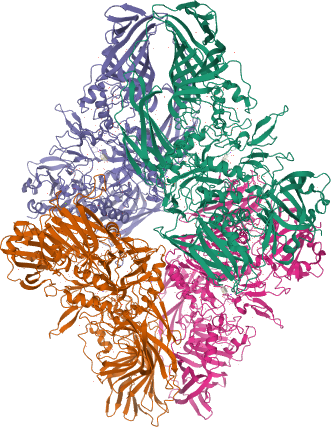
\includegraphics[height=3cm]{figures/5a1a_pdb.png}
            \caption{Atomic model of \texttt{5a1a}.}
        \end{subfigure}
        \hfill
        \begin{subfigure}[b]{0.49\linewidth}
            \centering
            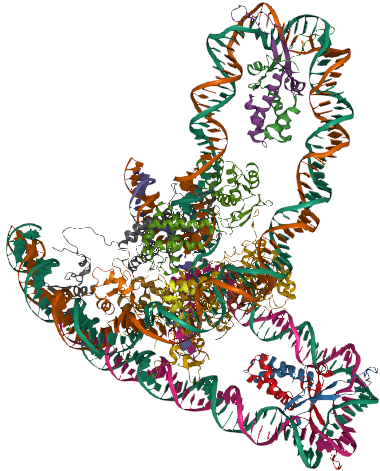
\includegraphics[height=3cm]{figures/5j0n_pdb_.png}
            \caption{Atomic model of \texttt{5j0n}.}
        \end{subfigure}
        \\ \vspace{0.5em}
        \begin{subfigure}[b]{0.49\linewidth}
            \centering
            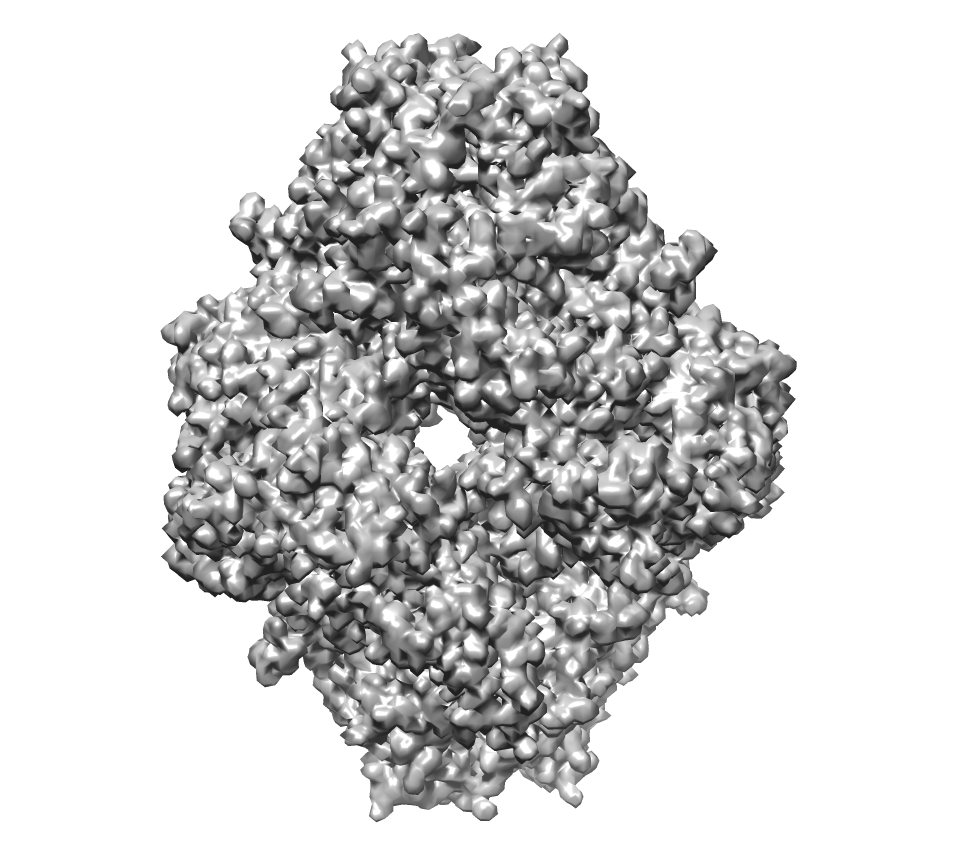
\includegraphics[height=3cm]{figures/5a1a_5A.png}
            \caption{5\AA\ density map $\x$ of \texttt{5a1a}.}%
            \label{fig:density-map:5j0n:ground-truth}
        \end{subfigure}
        \hfill
        \begin{subfigure}[b]{0.49\linewidth}
            \centering
            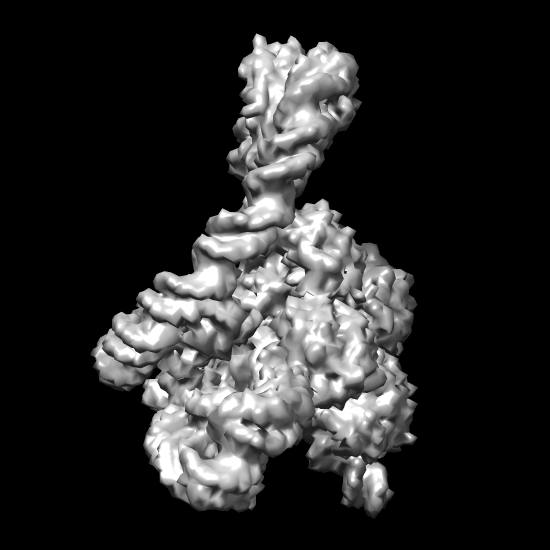
\includegraphics[height=3cm]{figures/5j0n_5A.png}
            \caption{5\AA\ density map $\x$ of \texttt{5j0n}.}
        \end{subfigure}
        \caption{%
            %A D2 symmetric (\texttt{5a1a}) and an asymmetric (\texttt{5j0n}) protein.
            Two proteins with different symmetries.
            %The $\beta$-galactosidase (\texttt{5a1a}) and the lambda excision HJ intermediate (\texttt{5j0n}).
        }\label{fig:pdb-proteins}
    \end{minipage}
    \hfill
    \begin{minipage}[b]{0.48\linewidth}
        \centering
        \begin{subfigure}[b]{0.49\linewidth}
            \centering
            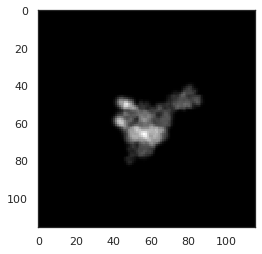
\includegraphics[height=3cm]{figures/5j0n_noise0}
            \caption{$\p = \mathbf{P}_{\bth} \mathbf{x}$}
        \end{subfigure}
        \hfill
        \begin{subfigure}[b]{0.49\linewidth}
            \centering
            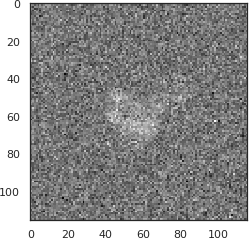
\includegraphics[height=3cm]{figures/5j0n_noise16}
            \caption{$\p = \mathbf{P}_{\bth} \mathbf{x} + \mathbf{n}$}
    %, \; \mathbf{n} \sim \mathcal{N}(0, 16\mathbf{I})$}
        \end{subfigure}
        \\ \vspace{0.5em}
        \begin{subfigure}[b]{0.49\linewidth}
            \centering
            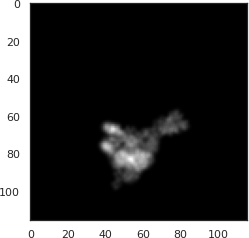
\includegraphics[height=3cm]{figures/5j0n_translated}
            \caption{$\p = \mathbf{S}_{\mathbf{t}} \mathbf{P}_{\bth} \mathbf{x}$}
        \end{subfigure}
        \hfill
        \begin{subfigure}[b]{0.49\linewidth}
            \centering
            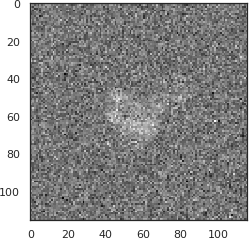
\includegraphics[height=3cm]{figures/5j0n_noise16_translated}
            \caption{$\p = \mathbf{S}_{\mathbf{t}} \mathbf{P}_{\bth} \mathbf{x} + \mathbf{n}$}
        \end{subfigure}
        \caption{%
            Example projections of \texttt{5j0n} ($\mathbf{n} \sim \mathcal{N}(0, 16\mathbf{I})$).
            % (a)~unperturbed, (b)~noisy, (c)~shifted, (d)~noisy and shifted.
        }\label{fig:different-projections}
    \end{minipage}
\end{figure}

\paragraph{Orientations.}
Symmetries are problematic to learn distances: two projections can be identical while not having been acquired from the same orientation---breaking an axiom of proper distance functions.
\figref{euclidean-not-robust:5a1a} illustrates the problem.
To capture only one of four identical projections of \texttt{5a1a}, we restricted directions to $(\theta_2, \theta_1) \in [0, \pi[ \, \times \, [0, \frac{\pi}{2}[$, a quarter of the sphere as illustrated in \figref{orientation-constraints}, for that protein.
% Symmetry group of order 4: 4 identical subunits, 4 orientations that yield the same projection.
% (a quarter of the sphere, We would restrict directions to an half (of the sphere) for a protein with C2 symmetry.)
%Symmetries aren't an issue beyond distance learning: orientations will be recovered over one of the four identical subunits of \texttt{5a1a}.
% projections from identical parts of a protein will collapse be identified upon orientation recovery.
% close projections whose orientations are far due to a symmetry will be recovered as being
% symmetries/projections will collapse/overlap/be identified/grouped
% indicating the symmetries. The reconstructed subunit can then be copied over.
% \ie, it is composed of four identical sub-units with two rotations of magnitude $\pi$ radians around the first axis followed by $\pi$ radians rotation around second axis, as illustrated and explained in~\cite{symmetry_in_protein,symmetry,scipion-em-github, rcsb-symmetry-view, EmpereurMot2019GeometricDO}.
This treatment of symmetries is incomplete\footnote{\todo{Explain.}} but sufficient for a proof-of-concept.

\paragraph{Projections.}
Using the ASTRA projector~\cite{van2015astra}, we generated $P=5,000$ synthetic projections of $275 \times 275$ pixels for \texttt{5a1a} and $116 \times 116$ pixels for \texttt{5j0n}, taken from uniformly sampled orientations.%
\footnote{Orientations used in \secref{results:orientation-recovery:sensitivity} (\figref{perfect-with-noise-ar-aa}) and \secref{results:distance-estimation:sensitivity} (\figref{results:distance-estimation}) were actually obtained by uniformly sampling the Euler angles $\bth$, constrained to $(\theta_3,\theta_2,\theta_1) \in [0, 2\pi[ \, \times \, [0, \frac{\pi}{2}[ \, \times \, [0, 2\pi[$ for \texttt{5j0n}. Our conclusions would be identical if orientations were uniformly sampled from $\SO(3)$ instead.}
%\banjac{I remember putting somewhere that we have support for both, but I don't see it. I can put a histogram and respective $S^2$ space visualization in the appendix that will visualize the difference. Why we used it? From the log I see that OR was not converging to 0 so we thought is is because we have underestimated learned distance. Shortly after, the OR started working and we didn't continue further with this idea.}
We then perturbed the measurements with different levels of additive Gaussian noise~\cite{sorzano2004normalizing,shigematsu2013noise} and off-centering shifts. %, (iii) inclusion of the effects of the point-spread functions (PSF).
%The mathematical formulation of these three components is given in \eqnref{imaging-model}.
\figref{different-projections} displays samples of the simulated projections.

% From projections to pairs and subsets (which are used for distance learning and orientation recovery).
\paragraph{Datasets.}
For each protein, we split the projections into training, validation, and test subsets; and created \textit{disjoint} pairs of projections from each (\tabref{dataset}).
% which are used as input to the SiameseNN, and as output their respective quaternion distances (calculated from their orientations);
The training and validation sets were used to train and evaluate the SiameseNN, while the test set was used to evaluate orientation recovery given a trained SiameseNN.
%\banjac{Actually, train and validation sets are used in distance learning, and test set was only used for dPdQ plot, orientation recovery (and alignment).}
%to ensure that it did not include any projection that was previously seen during the distance learning.
%Note that we split the $P=5,000$ projections, not the $P^2 = 25 \times 10^6$ possible pairs, to ensure we evaluate generalization to unseen projections.
% The sampling of orientations only matter for orientation recovery (test set).
% For distance learning (training and validation sets),
Figures~\ref{fig:orientation-sampling:distances} and~\ref{fig:orientation-constraints:distances} show that (mostly) uniform distributions of orientations induce distributions of distances that are skewed towards larger distances.
As this would skew $L_\text{DE}$ and bias $\widehat{d_p}$, we further sampled $1\%$ of the training and validation pairs to make the distribution of distances uniform---for $\widehat{d_p}$ to be uniformly accurate over the whole $[0,\pi]$ range of distances.
% such that the distribution of distances was uniform (independently from the distribution of orientations)
% The goal was to uniformly spread the distance estimation error over the range of distances.
%\mdeff{So those pairs are sampled from $63,126$ pairs from the training dataset, rather than the $P^2$ possible pairs? If true, we should motivate somewhere why we limit our training dataset.}
%We restricted the size of our training and validation datasets due to Google Colaboratory\footnote{A hosted Jupyter notebook service from Google Research with resources that are not guaranteed and not unlimited.} training time limit of 12 hours.
%\mdeff{No. 100 epochs over 1% takes the same time as 1 epoch over 100%.}
See \apxref{orientation-sampling} for further illustrations.
While $1,650$ projections were enough to perfectly reconstruct 5\AA\ density maps,\footnote{We obtained an \todo{FSC of 1 across frequencies} by reconstructing from $1,650$ projections and their true orientations.} our method is not limited by the number of projections as optimization is done per batch.

\paragraph{Optimization.}
%\todo{Jelena: check the settings, make sure they are used for all experiments, and add anything missing?} \banjac{Checked, yes, parameters are the same.}
We optimized \eqnref{distance-learning} with the RMSProp optimizer~\cite{tieleman2012rmsprop} and a learning rate of $10^{-3}$ for $150$ epochs.
With batches of $256$ pairs, that was $247$ steps per epoch for the training sets and $28$ for the validation sets (\tabref{dataset}).
It took about $3.3$ hours of a single Tesla T4 or $8.75$ hours of a single Tesla K40c. Our code can train faster on multiple GPUs.
% 2.6 to 9.3 hours depending on available resources.
% \mdeff{We just want a ball-park (\eg, not a day or a week).}
We optimized \eqnref{orientation-recovery} with the Adam optimizer~\cite{kingma2014adam} and a learning rate of $0.5$ until convergence on batches of $256$ pairs sampled from the test sets (\tabref{dataset}).
It took about $3.75$ hours of a single Tesla K40c (without early stopping).
%Unlike distance learning algorithm, the orientation recovery optimization does not support multi-GPU execution.
We optimized \eqnref{orientation-recovery-error} with the FTRL optimizer~\cite{mcmahan2013ftrl}, a learning rate of $2$, and a learning rate power of $-2$ on batches of $256$ orientations sampled from the test sets (\tabref{dataset}).
We reported the lowest of 6 runs (3 per value of $m$) of 300 steps each.
It took about 50 minutes of CPU.
% 8 minutes per run => 6*8 = 48 minutes
% ($\sim$ 50 minutes in the best resource availability setting)

%%%%%%%%%%%%%%%%%%%%%%%%%%%%%%%%%%%%%%%%%%%%%%%%%%%%%%%%%%%%%%%%%%%%%%%%%%%%%%%%%%%%%%%

%\subsubsection{Robustness of Recovery to Additive Errors on the Relative Distances}
\subsection{Sensitivity of orientation recovery to errors in distance estimation}\label{sec:results:orientation-recovery:sensitivity}

%\mdeff{Story: (i) orientation recovery error is strongly linked to distance estimation error, (ii) recovery loss is a good proxy of mean recovery error.}
%\mdeff{Story: good distance estimation = good orientation recovery.}

We first evaluated the feasibility of orientation recovery assuming that the exact distances between pairs were known.
Experiments confirmed that the method successfully recovers the orientation of every projection in this case (see \apxref{results:orientation-recovery:exact}).

We then evaluated the behavior of~\eqnref{orientation-recovery} when the true distances were increasingly perturbed.
More precisely, we perturbed the distances prior to the minimization with an error sampled from a Gaussian distribution with mean $0$ and variances $\sigma^2 \in [0.0, 0.8]$.
\figref{perfect-with-noise-ar-aa} shows that the recovery error $E_\text{OR}$ from \eqnref{orientation-recovery-error} is a monotonic function of the error in distances: from $E_\text{OR} = 0$ with perfect distances to $E_\text{OR} \approx 0.2$ radians ($\approx 11.5\degree$) for $\sigma^2 = 0.8$.
% represented as the variance $\sigma^2$ of white noise added to the true distances.
%More accurate distance estimation leads to more accurate orientation recovery,
These results demonstrate that the performance of orientation recovery~\eqnref{orientation-recovery} depends on the quality of the estimated distances, which advocates for a proper and extensive training of the SiameseNN in further stages of development.

Moreover, we observe that the loss $L_\text{OR}$ from \eqnref{orientation-recovery} is a reliable proxy for $E_\text{OR}$, allowing us to assess recovery performance in the absence of ground-truth orientations (\ie, when recovering the orientations of real not simulated projections).
%Hence, it suggests that the loss can be used as a good indicator of its performance, as it shows how well the proposed method works even if the true distances are not available.
%Hence, it has practical implications for our future works on real data.

\begin{figure}
    \begin{minipage}[b]{0.48\linewidth}
        \begin{minipage}{\linewidth}
            \begin{tabular}{lrrr}
                \toprule
                %Dataset & Number of projections $P$ & Maximum number of pairs $P^2$ & Used number of pairs \\
                Dataset & $P$ & $P^2$ & Used pairs \\
                \midrule
                Training & 2,512 (50\%) & 6,310,144 & 63,101 \\ % (1\%) \\
                Validation & 838 (17\%) & 702,244 & 7,022 \\ % (1\%) \\
                Test & 1,650 (33\%) & 2,722,500 & 2,722,500 \\ % (100\%) \\
                \bottomrule
            \end{tabular}
            \captionof{table}{%
                Split of $P=5,000$ projections in training, validation, and test subsets.
                %\mdeff{The number of pairs is given by $(P^2-P)/2$, not $P^2$ or $P^2-P$. Because pairs are made of distinct projections and order doesn't matter. Did we sample with those constraints?}
                %\banjac{thanks for remark, and I totally agree we need to use combinations of 2, however, I checked (and didn't notice before) that we use $P^2$ :(}
                %\mdeff{It's actually good to train on identity to force zero distance. And order doesn't matter, so no problem.}
            \vspace{2.5em}
            }\label{tab:dataset}
        \end{minipage}
        \begin{subfigure}[b]{0.49\linewidth}
            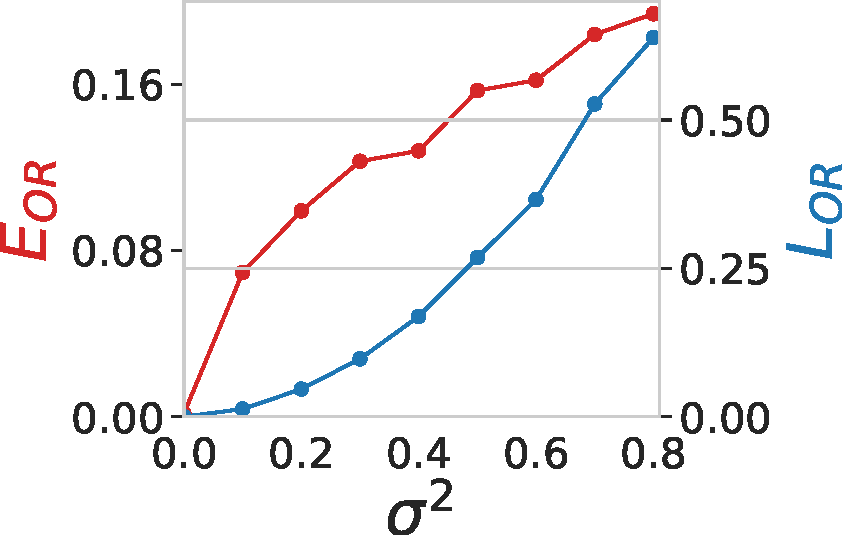
\includegraphics[width=\linewidth]{figures/5j0n_perfect_noisy_ar_aa}
            \caption{Recovering from \texttt{5j0n}.}
        \end{subfigure}
        \hfill
        \begin{subfigure}[b]{0.49\linewidth}
        \centering
            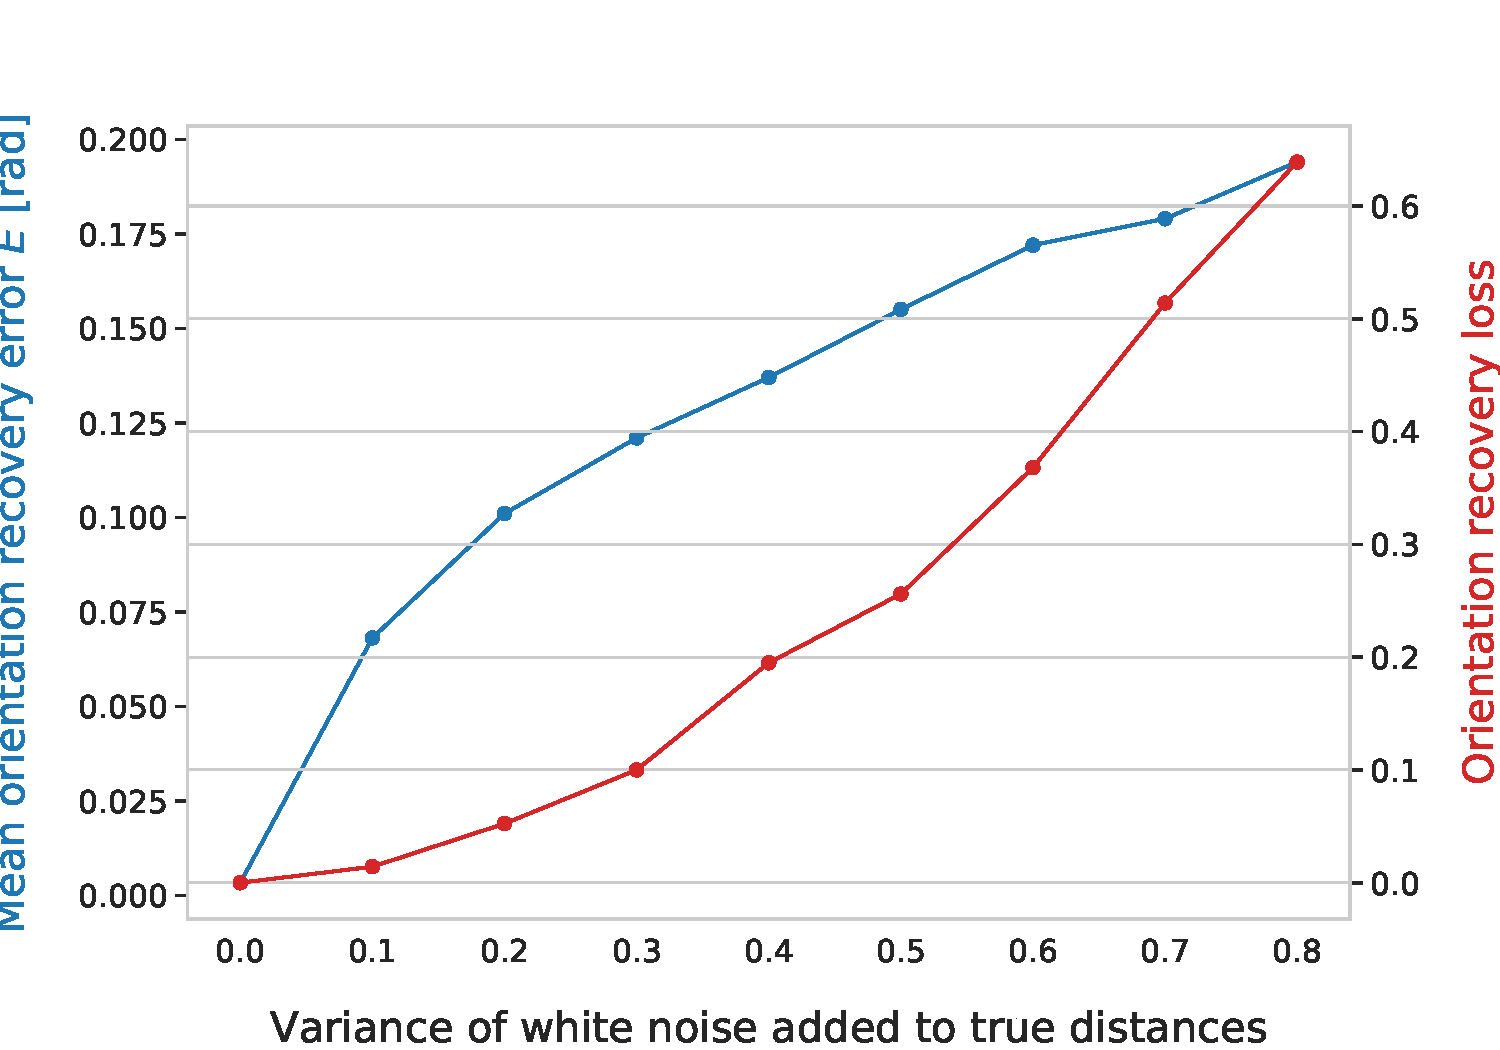
\includegraphics[width=\linewidth]{figures/5a1a_perfect_noisy_ar_aa}
            \caption{Recovering from \texttt{5a1a}.}
        \end{subfigure}
        \caption{%
            Orientation recovery from perturbed distances.
        }\label{fig:perfect-with-noise-ar-aa}
    \end{minipage}
    \hfill
    \begin{minipage}[b]{0.45\linewidth}
        \begin{subfigure}[b]{\linewidth}
            \centering
            %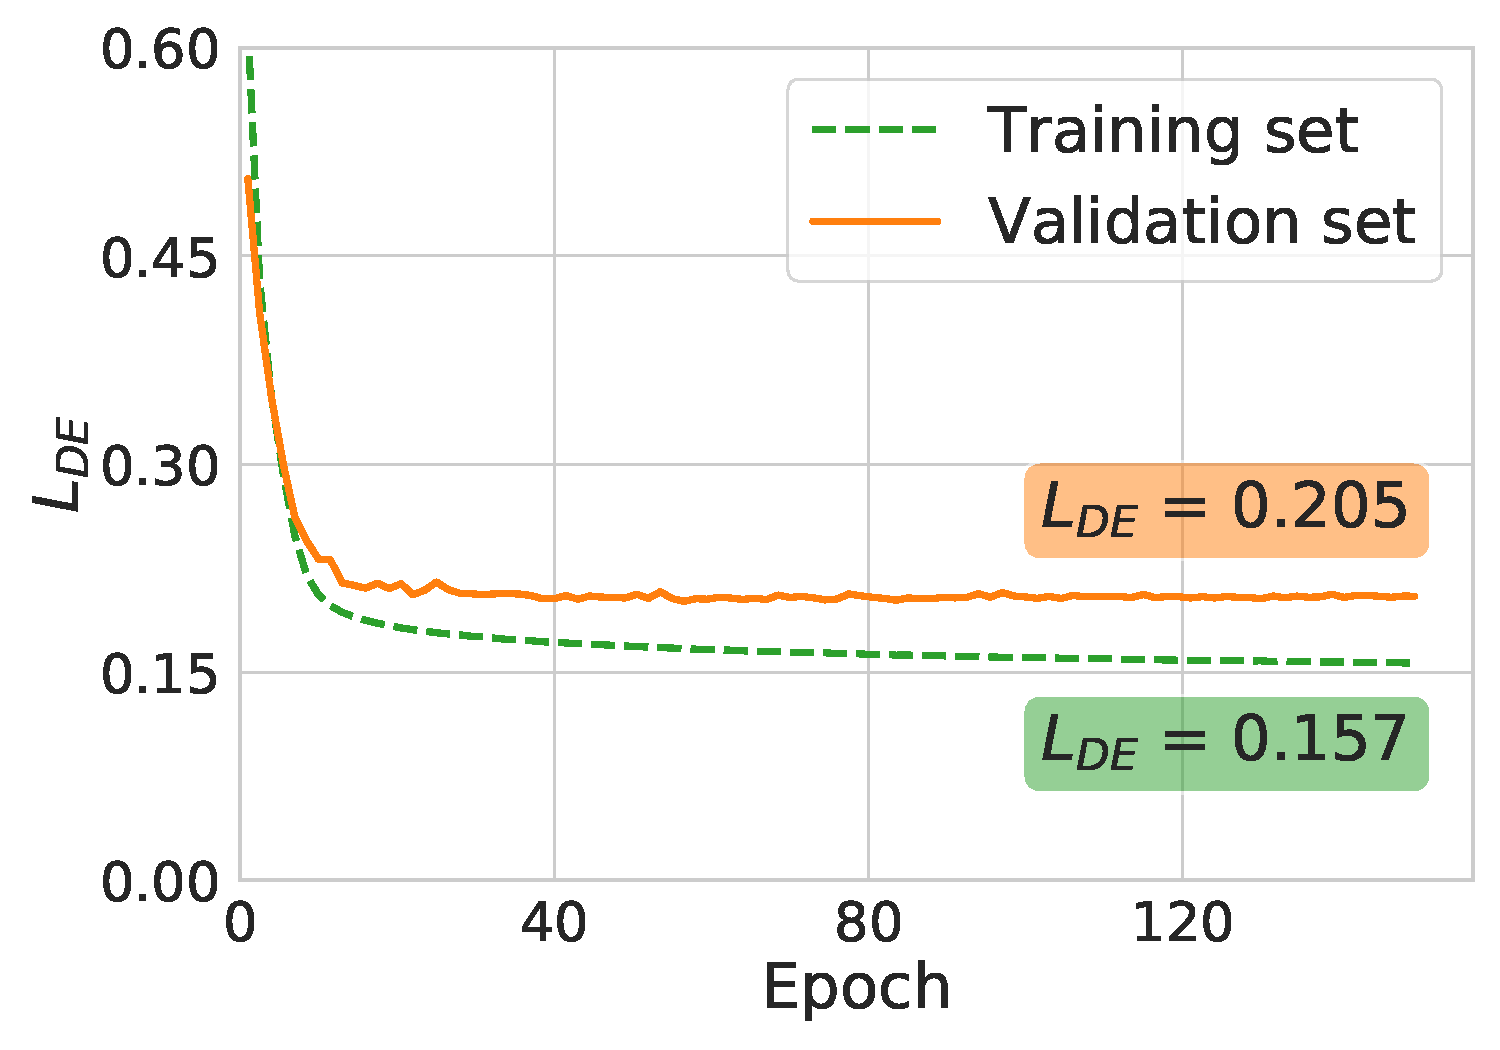
\includegraphics[width=0.47\linewidth]{figures/de_5j0n_fullcov.pdf}
            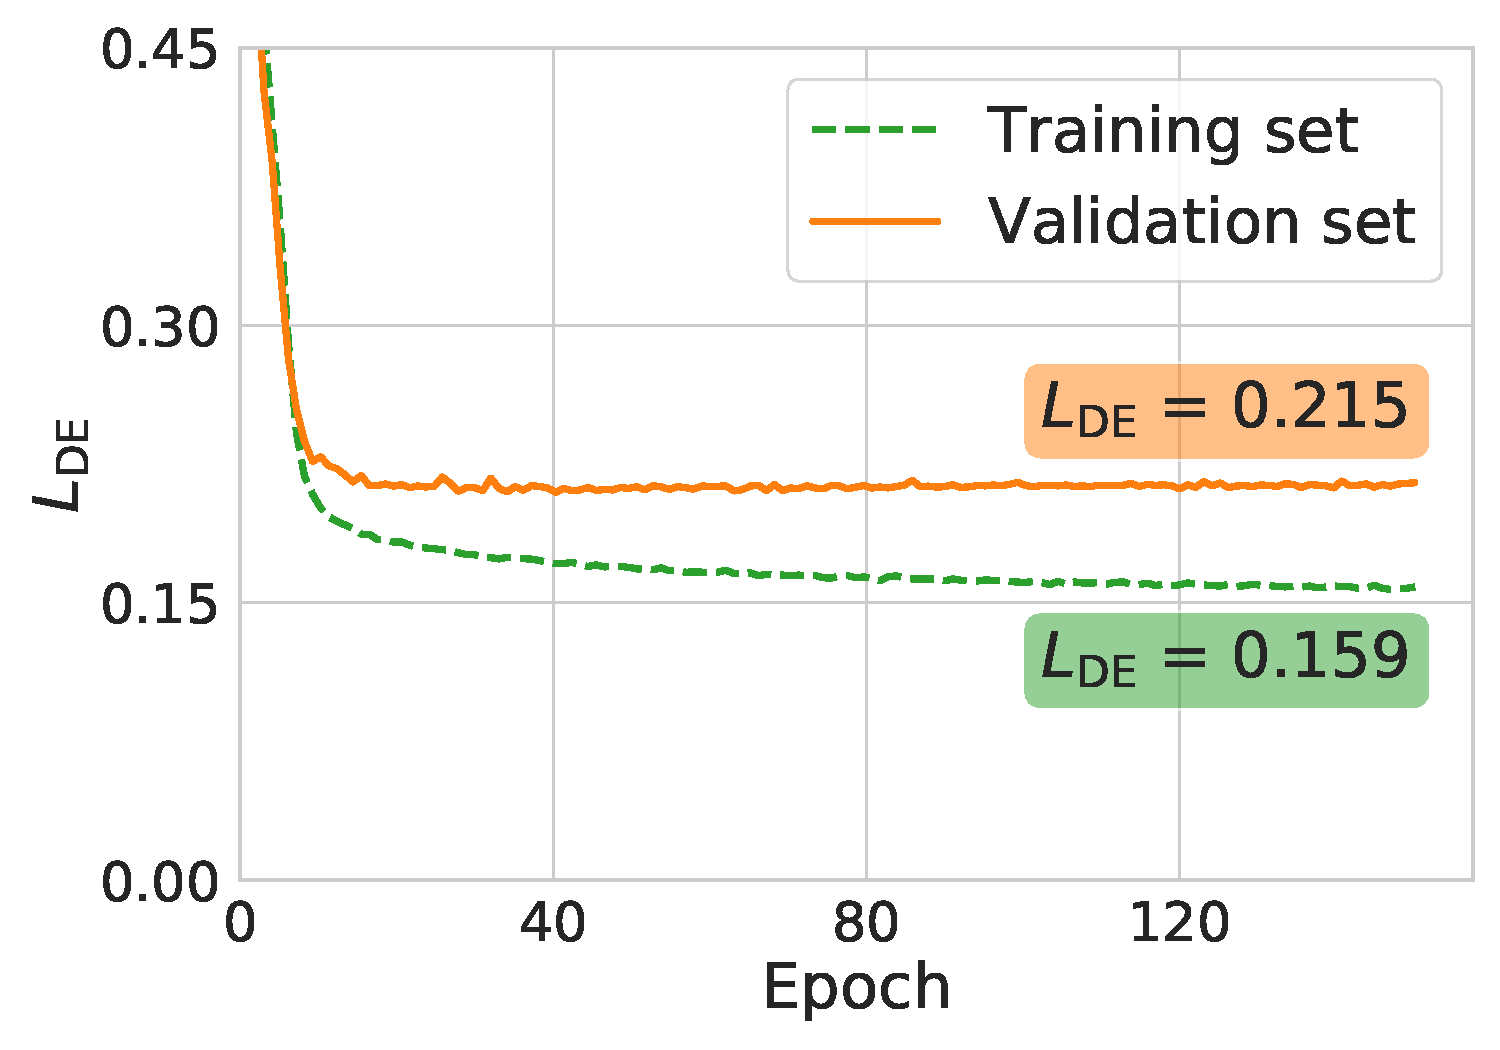
\includegraphics[width=0.47\linewidth]{figures/de_5j0n_fullcov_uniformS2.pdf}
            \hfill
            %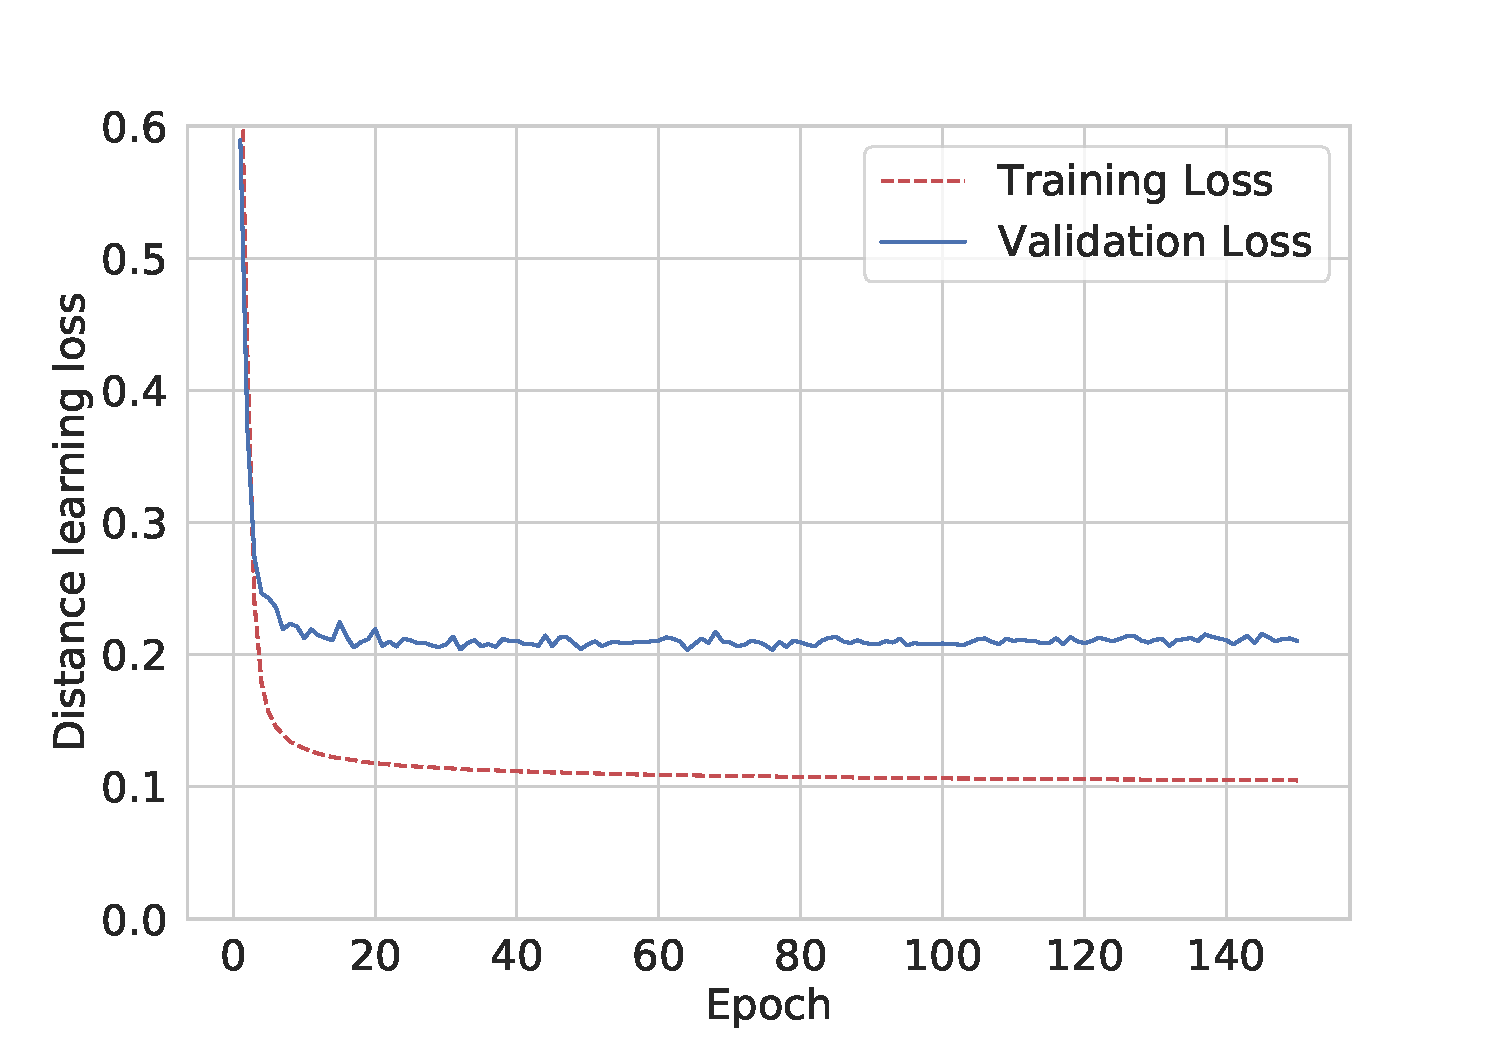
\includegraphics[width=0.47\linewidth]{figures/de_5a1a.pdf}  % old quarter coverage - 2, 0.4, 1
            %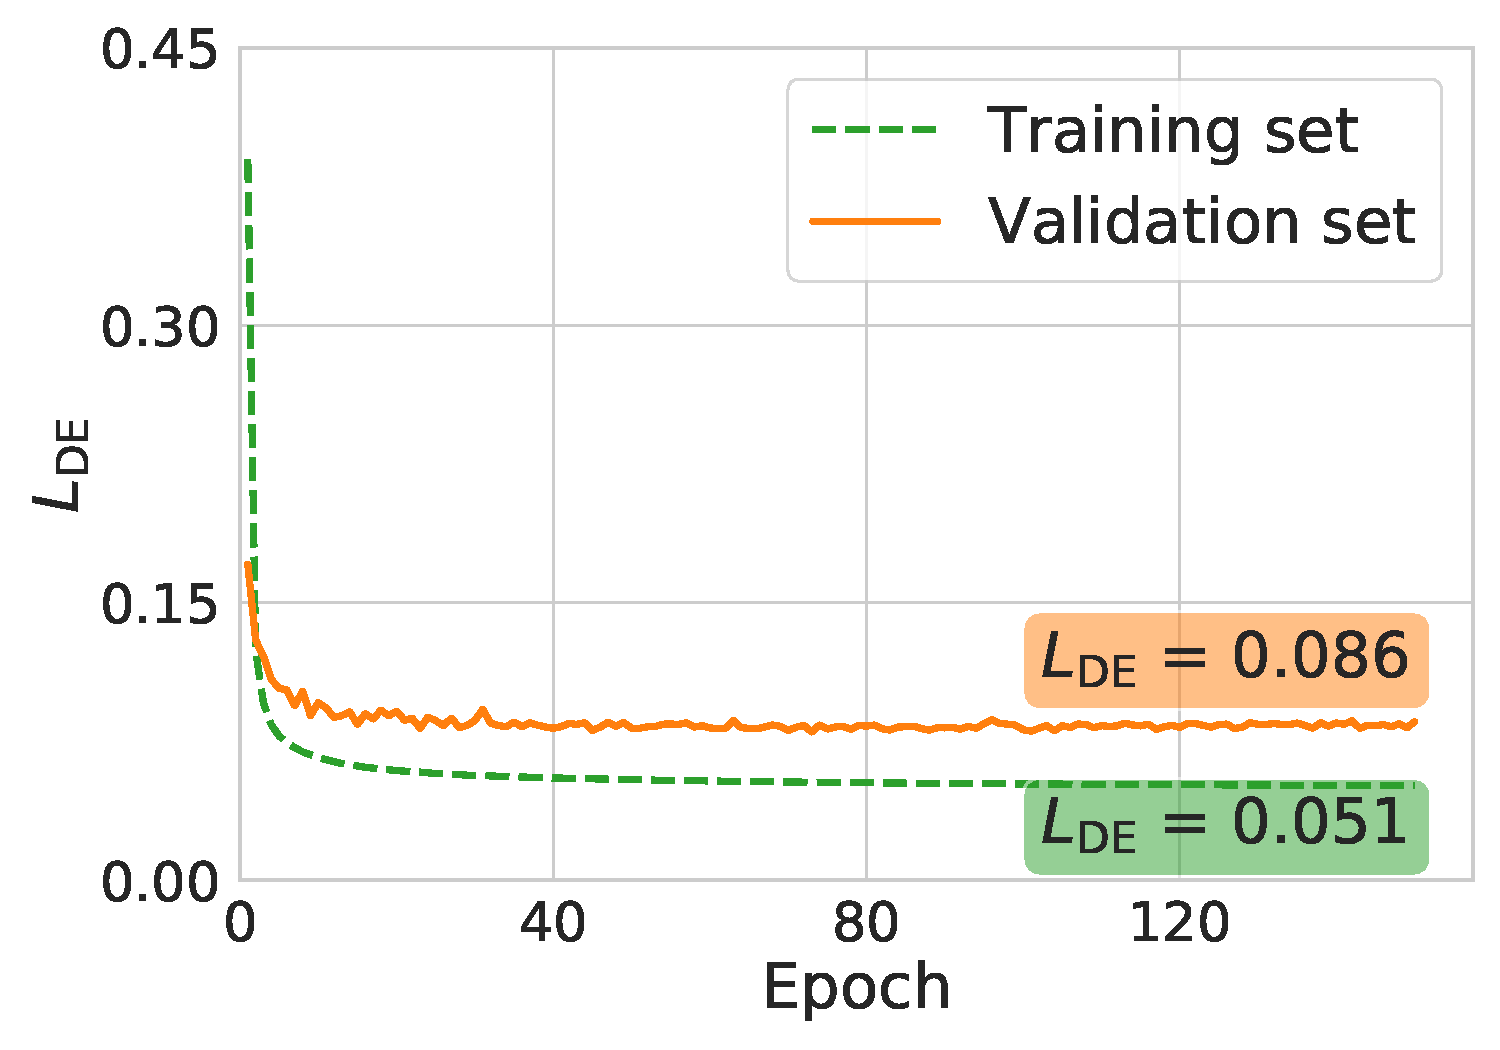
\includegraphics[width=0.47\linewidth]{figures/de_5a1a_quartercov_uniformS2.pdf}
            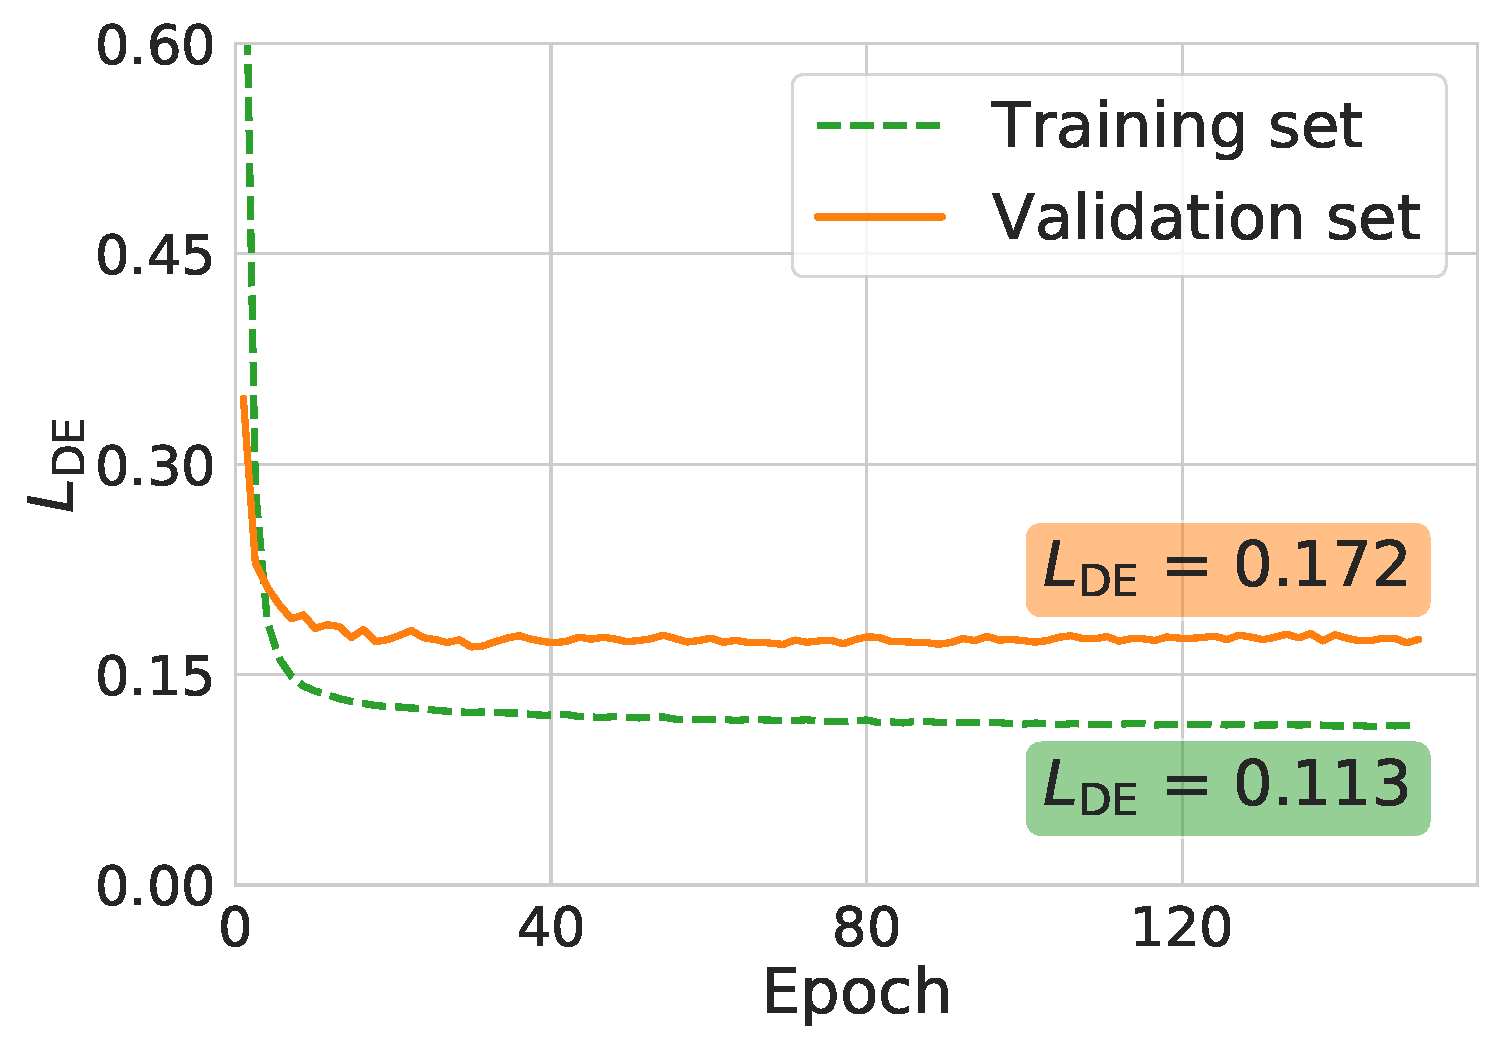
\includegraphics[width=0.47\linewidth]{figures/de_5a1a_last.pdf}  % latest correct quarter coverage - 2, 1, 0.4, but dPdQ was ran on full, now run it on quarter only
            \caption{Loss converged on \texttt{5j0n} (left) and \texttt{5a1a} (right).
            % \banjac{Fix \texttt{5a1a} plot y-axis.}
            \vspace{0.8em}}%
            \label{fig:distance-learning:loss}
        \end{subfigure}
        \\ %\vspace{1em}
        \begin{subfigure}[b]{\linewidth}
            \centering
            %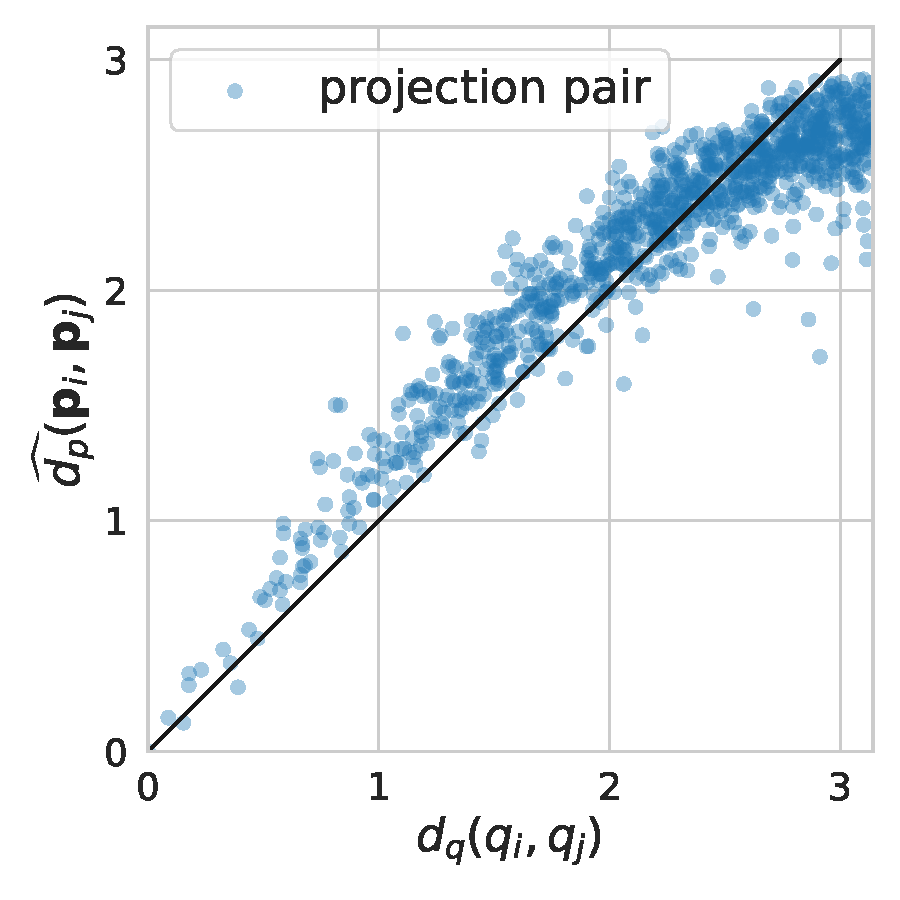
\includegraphics[width=0.40\linewidth]{figures/dPdQ_5j0n_fullcov.pdf}
            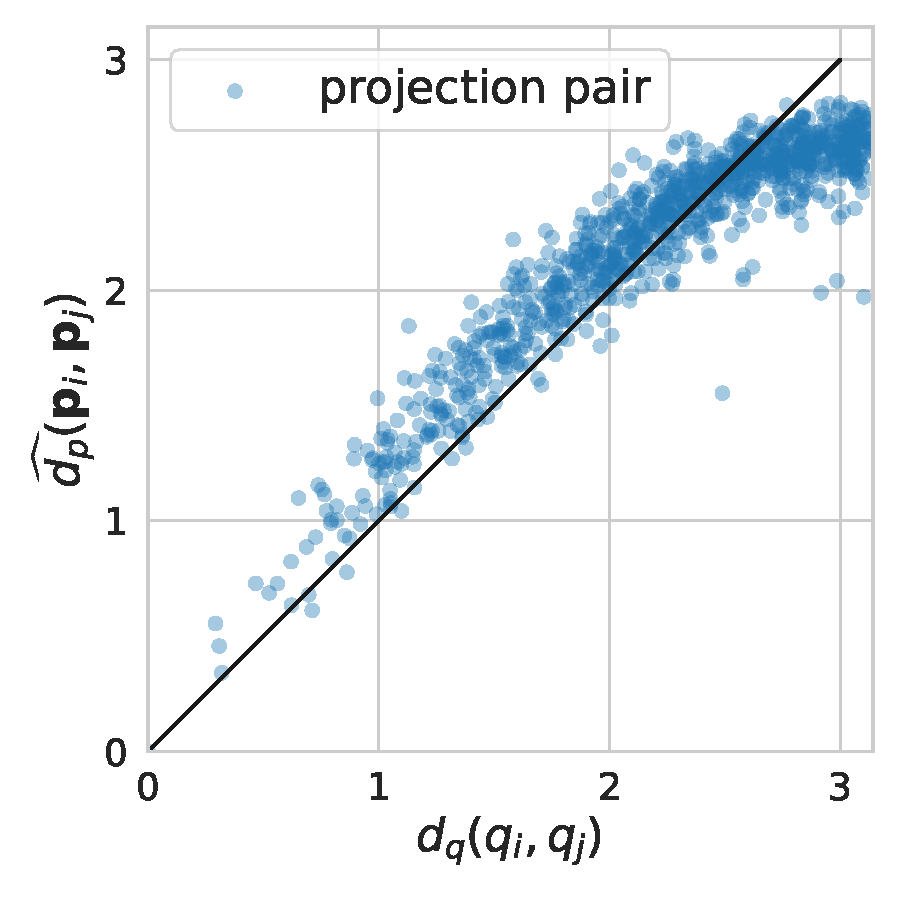
\includegraphics[width=0.40\linewidth]{figures/dPdQ_5j0n_fullcvg_uniformS2_noise0.pdf}
            \hspace{0.5cm}
            % 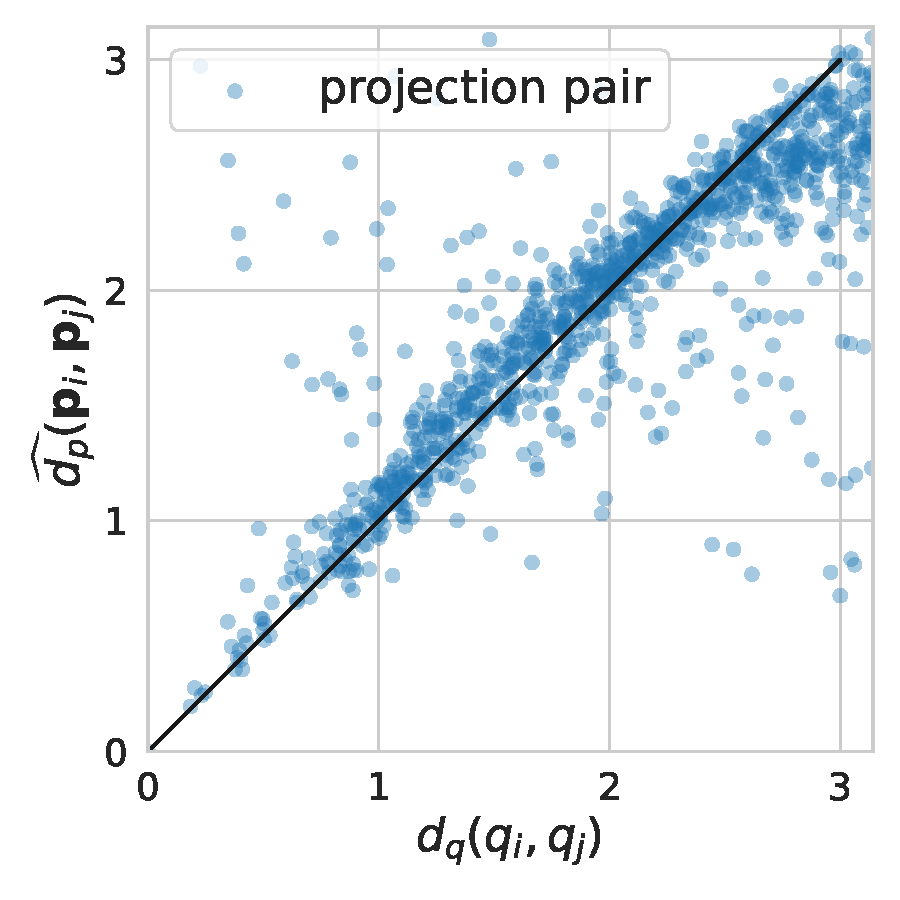
\includegraphics[width=0.40\linewidth]{figures/dPdQ_5a1a.pdf}  % old quarter coverage - 2, 0.4, 1
            %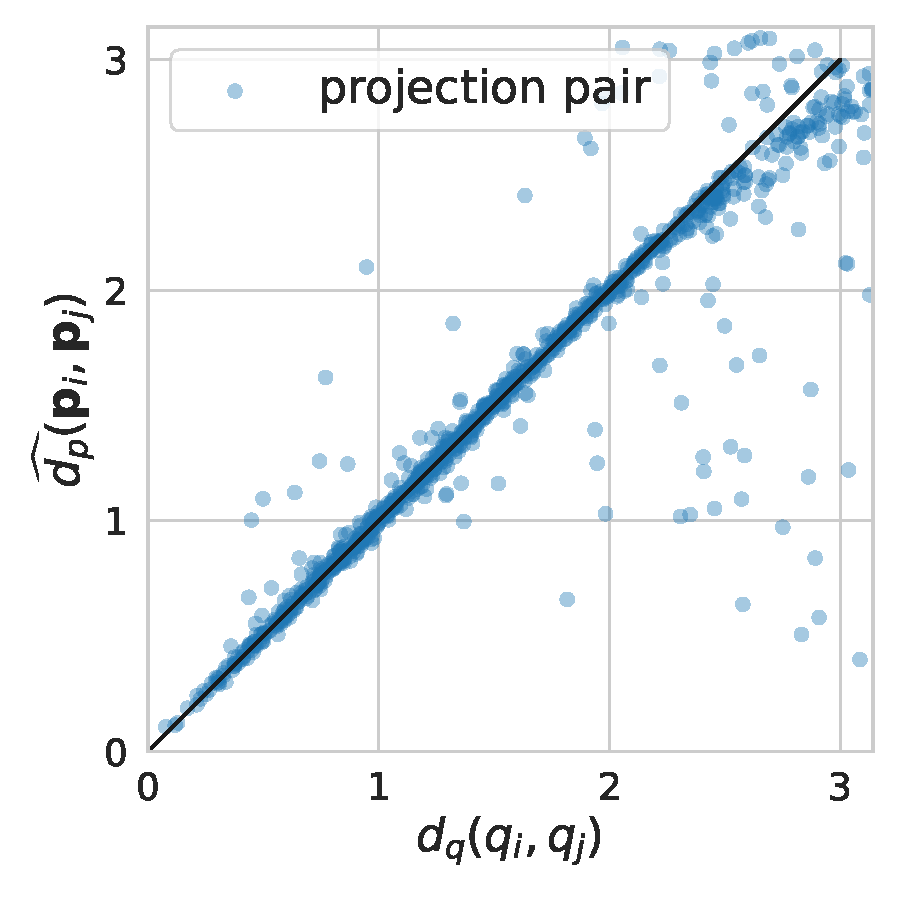
\includegraphics[width=0.40\linewidth]{figures/dPdQ_5a1a_quartercvg_uniformS2_noise0_halfInplane.pdf}
            %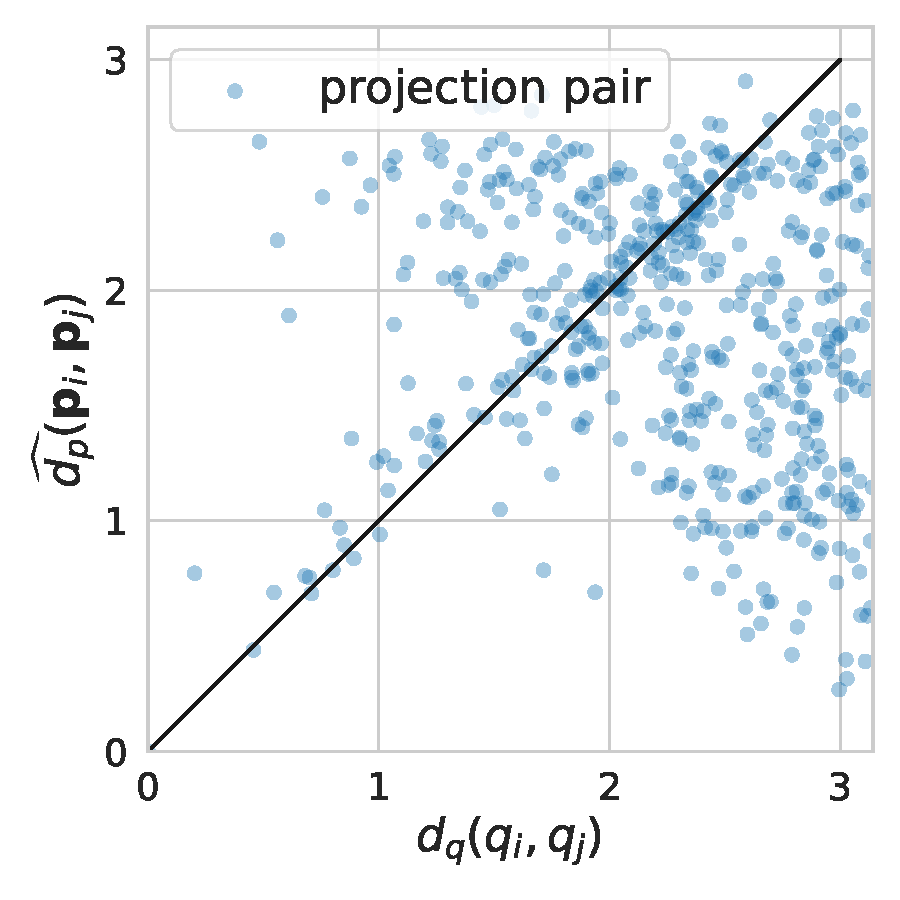
\includegraphics[width=0.20\linewidth]{figures/dPdQ_5a1a_quartercvg_uniformS2_noise0_1.pdf}
            %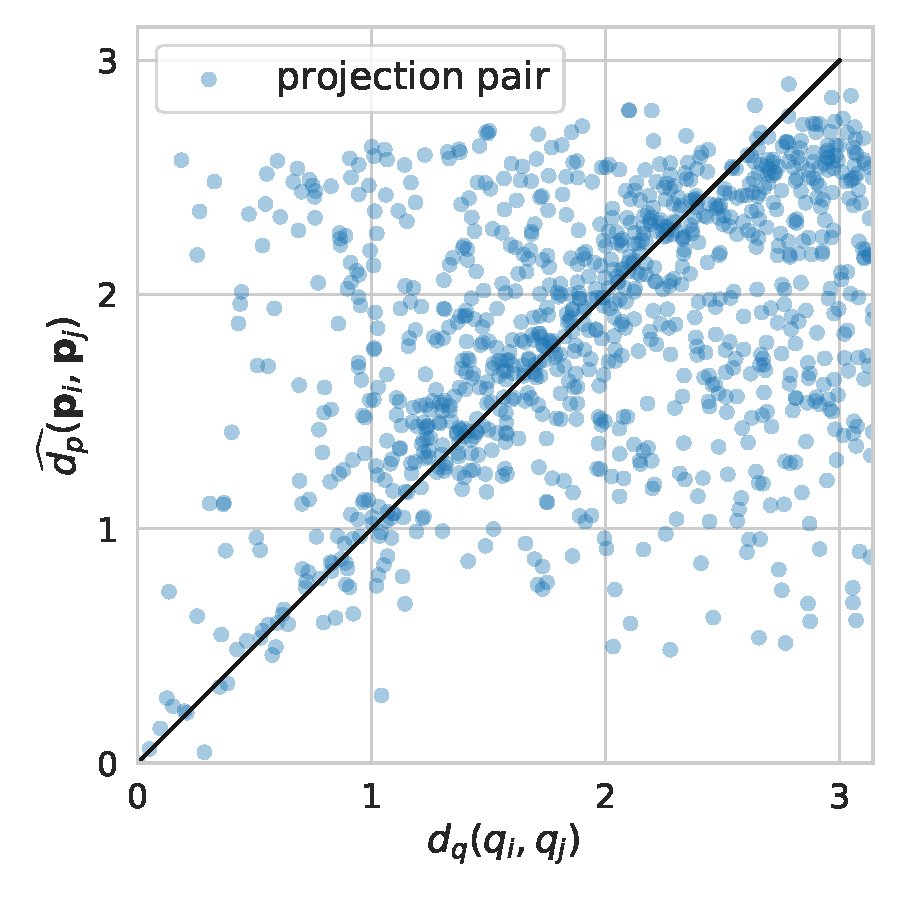
\includegraphics[width=0.20\linewidth]{figures/dPdQ_5a1a_quartercvg_uniformS2_noise0_2.pdf}
            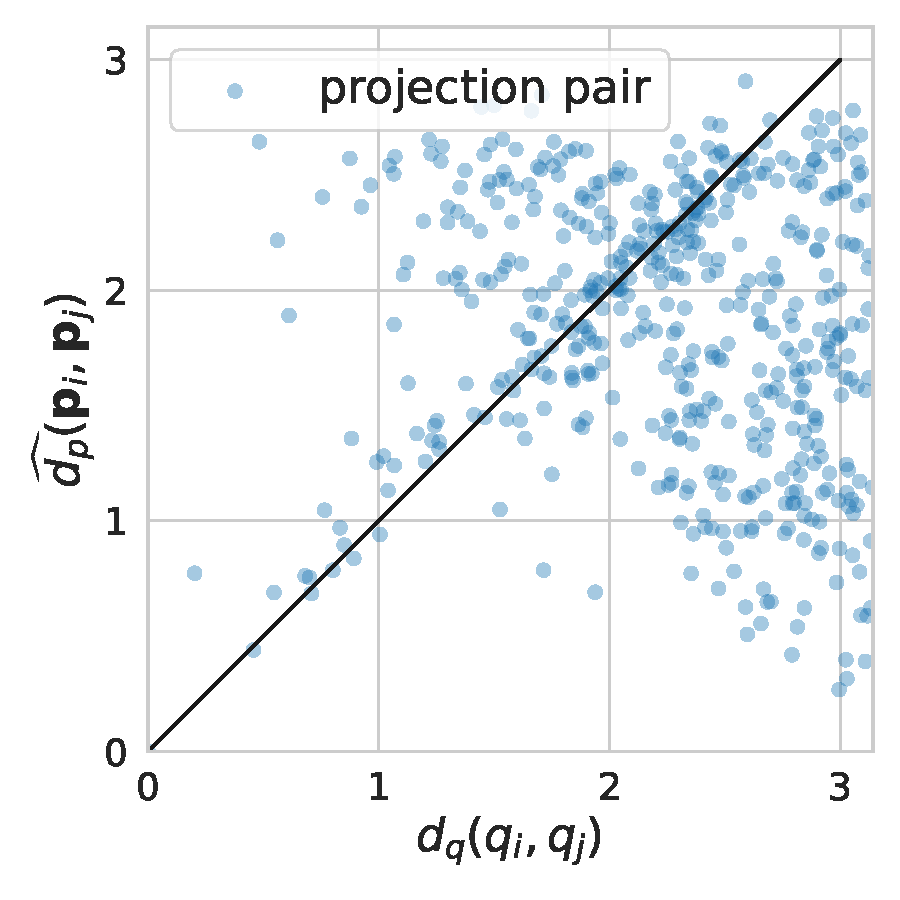
\includegraphics[width=0.40\linewidth]{figures/dPdQ_5a1a_quartercvg_uniformS2_noise0.pdf}
            \caption{Relationship between $\widehat{d_p}$ and $d_q$ on $1,000$ pairs sampled from the test sets of \texttt{5j0n} (left) and \texttt{5a1a} (right).
            }\label{fig:distance-learning:dpdq}
        \end{subfigure}
        \caption{Distance learning.
        %\banjac{To discuss which to use?}
        }
    \end{minipage}
\end{figure}

%%%%%%%%%%%%%%%%%%%%%%%%%%%%%%%%%%%%%%%%%%%%%%%%%%%%%%%%%%%%%%%%%%%%%%%%%%%%%%%%%%%%%%%

\subsection{Learning to estimate distances}\label{sec:results:distance-estimation:learned}
%\subsection{Learned function for distance estimation}
%\subsection{Estimating Relative Orientations from Projections}
%\subsection{Relative orientation estimation}

%\mdeff{Story: $d_p$ good estimator of $d_q$.
%SiameseNN better than l2, but still plateaus.
%Robust to projection noise.}

%\mdeff{Story: learned distance $d_{ps}$ estimates $d_q$ with some variance but still underestimates larger distances.
%Again symmetric vs asymmetric.}

We evaluated how well our SiameseNN could learn \eqnref{distance-learning} to approximate the orientation distance $d_q$.
% ---parameterized as a SiameseNN and trained---
% to learn a distance between projections $\widehat{d_p}(\p_i,\p_j)$
For comparison, we evaluated a baseline, the Euclidean distance $d_p(\p_i,\p_j) = \|\p_i, \p_j\|_2$, in \apxref{results:distance-estimation}.

\figref{distance-learning:loss} shows how $L_\text{DE}$ converged in about 50 epochs.
%\todo{Values: $L_\text{DE} = ?$ for training/validation and \texttt{5j0n}/\texttt{5a1a}.}
We observe that overfitting---the difference between training and validation losses---is larger for \texttt{5a1a} than \texttt{5j0n}.
A large overfitting indicates that the distance trained on projections drawn from training sets fail to generalize to unseen projections drawn from validation sets.
That is a first suggestion (see again in \secref{results:orientation-recovery:reconstruction}) that \texttt{5a1a} is harder than \texttt{5j0n}.
We have two hypotheses: Some proteins have 3D density maps whose projections with close orientations are harder to distinguish from one another.
% not hard symmetries, but similarities
%We might have miss-handled its symmetry (\secref{results:data}).
\todo{Think about this: why is \texttt{5a1a} harder than \texttt{5j0n}?}
% \mdeff{$275 \times 275$ vs $116 \times 116$ projection size? The former induces a larger average pooling size, \ie, it's harder for $\G_w$ to see more global features.}

%\todo{This is most likely due to the symmetry of the protein (even though a quarter-sphere coverage was used.
%Indeed, its synthetic dataset may still contain pairs of projections that share the same $d_p$, yet differ in their $d_q$.
%This  advocates for restricting to non-overlapping areas of $\SO(3)$ the sampling of the orientations used to generate the training dataset.
%The latter would then only contain projection pairs with a linear $(d_q,d_p)$ relationship, which should ensure a successful training of the network.}

\figref{distance-learning:dpdq} shows the relationship between the distance $\widehat{d_p}$ estimated from projections and the true distance $d_q$.
As expected, distances were better estimated for \texttt{5j0n} than \texttt{5a1a}.
While our learned distance function is a much better estimator than the Euclidean distance---compare \figref{distance-learning:dpdq} with \figref{euclidean-not-robust}---they share one characteristic: both plateau and underestimate the largest distances.
We did attenuate the phenomenon by sampling training distances uniformly (see \secref{results:data}), and the issue is much less severe than with the Euclidean distance.
%\todo{Hypotheses: Because the true distances are upper-bounded by $\pi$? Training?}
%While the impact on orientation recovery is unclear
An alternative could be to discard larger distances and only rely on smaller distances for recovery.
That would however require the addition of a spreading term in \eqnref{orientation-recovery} to prevent the recovered orientations to collapse.
Outliers are explained by our incomplete treatment of symmetries.

% proxy distance
These results confirm that a SiameseNN is able to estimate differences in orientations from projections alone.
They are encouraging; indeed, much has yet to be gained from improving upon the rather primitive SiameseNN architecture we are currently using.
Moreover, more training data will diminish overfitting.
% Recurring theme.

%%%%%%%%%%%%%%%%%%%%%%%%%%%%%%%%%%%%%%%%%%%%%%%%%%%%%%%%%%%%%%%%%%%%%%%%%%%%%%%%%%%%%%%

\subsection{Sensitivity of distance learning to perturbations in the projections}\label{sec:results:distance-estimation:sensitivity}
%\subsection{Generalization of distance learning}
%\subsection{Generalizability/Abstractability of distance learning}

%\mdeff{Story: learned distance is minimally sensible to perturbations (additive noise, shift, PSF) because we can train it to ignore irrelevant information.
%Thanks again to good model of cryo-EM imaging.}

% Intro and shift.
We desire to estimate distances that are invariant to perturbations in the projections---specified in~\eqnref{imaging-model}.
As discussed in \secref{method:distance-learning}, the convolutional architecture of the SiameseNN should be shift invariant.
\figref{results:distance-estimation:shift} indeed shows that learning distances (and hence recovering orientations) is insensible to off-centering shifts.

% Noise.
As we cannot---or do not yet know how to---build noise invariance into the architecture, we trained the SiameseNN on noisy projections and evaluated whether it could learn to ignore noise as being irrelevant information.
% brute force vs principled engineering
\figref{results:distance-estimation:noise} shows $E_\text{OR} \approx 0.16$ radians ($\approx 9\degree$) for noiseless projections and $E_\text{OR} \approx 0.42$ radians ($\approx 24\degree$) for a more realistic noise variance of $\sigma^2=16$.
\mdeff{Shall we characterize the noise level with a signal-to-noise ratio? What $\sigma$ or SNR should we expect with real data? To help readers put our reported performance in context.}
%\mdeff{How good is that?}\banjac{To be discussed tomorrow}\lau{Reasonable first guess, room for improvement.}
While a naive distance function (like an Euclidean distance) would be tremendously sensitive to noise, the SiameseNN mostly learned to discard it.
Moreover, overfitting (\ie, the growing gap between the validation and training losses) indicates that more training data will further decrease the SiameseNN's sensitivity to noise.

% PSF and conclusion.
We didn't evaluate sensitivity to the PSF but expect a similar behavior.
%While we would ideally want the NN architecture to be engineered to ignore irrelevant information, that is not always possible.
%We know how to do it for shifts, not noise or PSF.

We observe again (\secref{results:orientation-recovery:sensitivity}) that (i) the estimation of more accurate distances (a smaller $L_\text{DE}$) leads to the recovery of more accurate orientations (a smaller $L_\text{OR}$ and $E_\text{OR}$), and (ii) that an higher recovery loss $L_\text{OR}$ induces an higher error $E_\text{OR}$.

\begin{figure}[ht!]
    \centering
    \begin{subfigure}[t]{0.47\linewidth}
        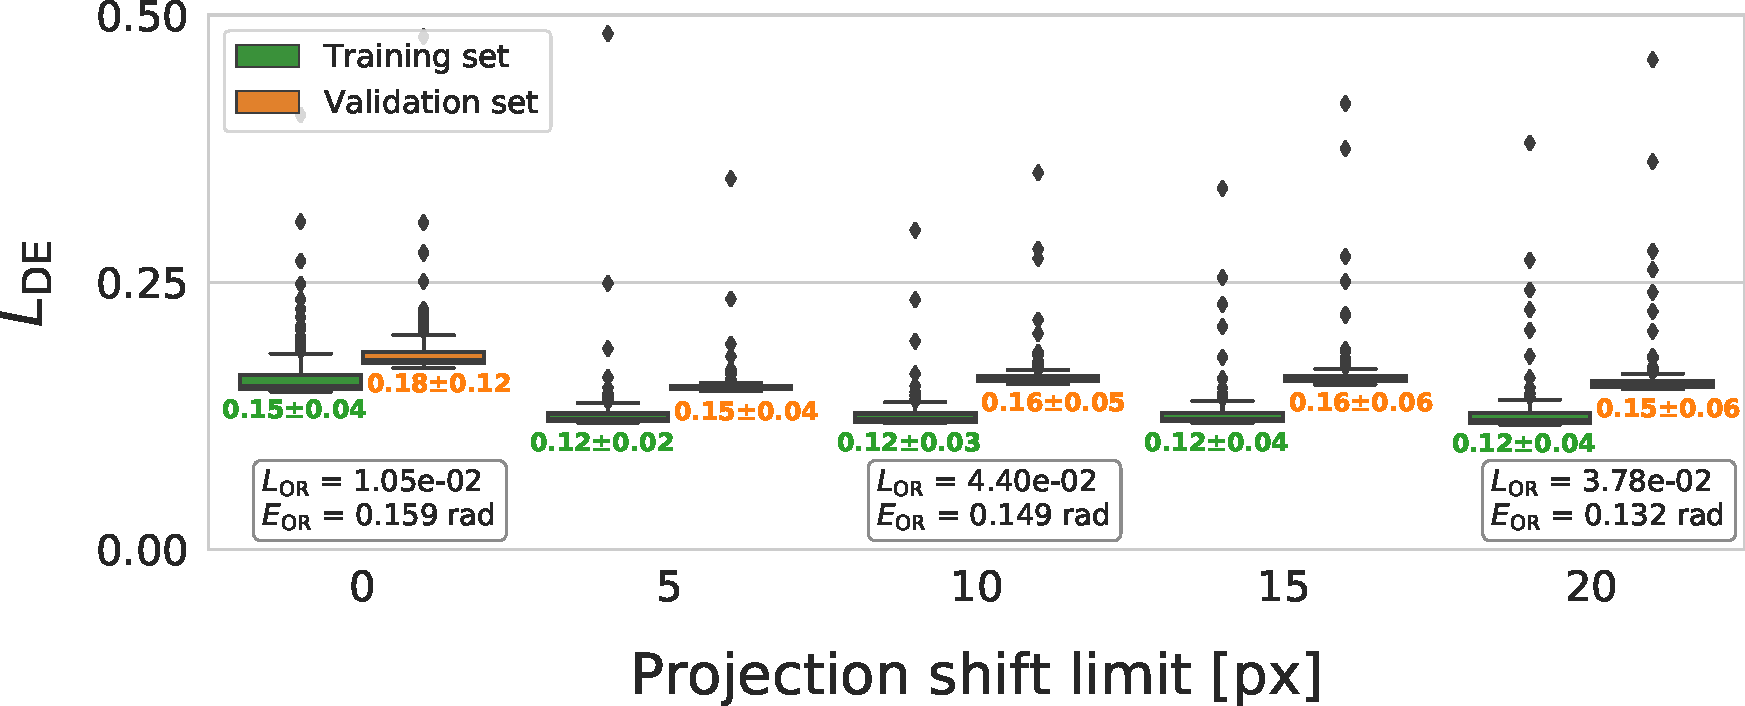
\includegraphics[width=\linewidth]{figures/de_translation_nums}
        \caption{%
            Learning from shifted projections $\{ \mathbf{S}_{\mathbf{t}_i} \mathbf{P}_{\bth_i} \mathbf{x} \}$, with shifts $t_{i_1}$ and $t_{i_2}$ sampled from a triangular distribution with mean 0 and of increasing limits.
            Learning is not harder as projections get shifted farther, because shift invariance is built into the convolutional architecture of $\mathcal{G}_w$.
    }\label{fig:results:distance-estimation:shift}
    \end{subfigure}
    \hfill
    \begin{subfigure}[t]{0.47\linewidth}
        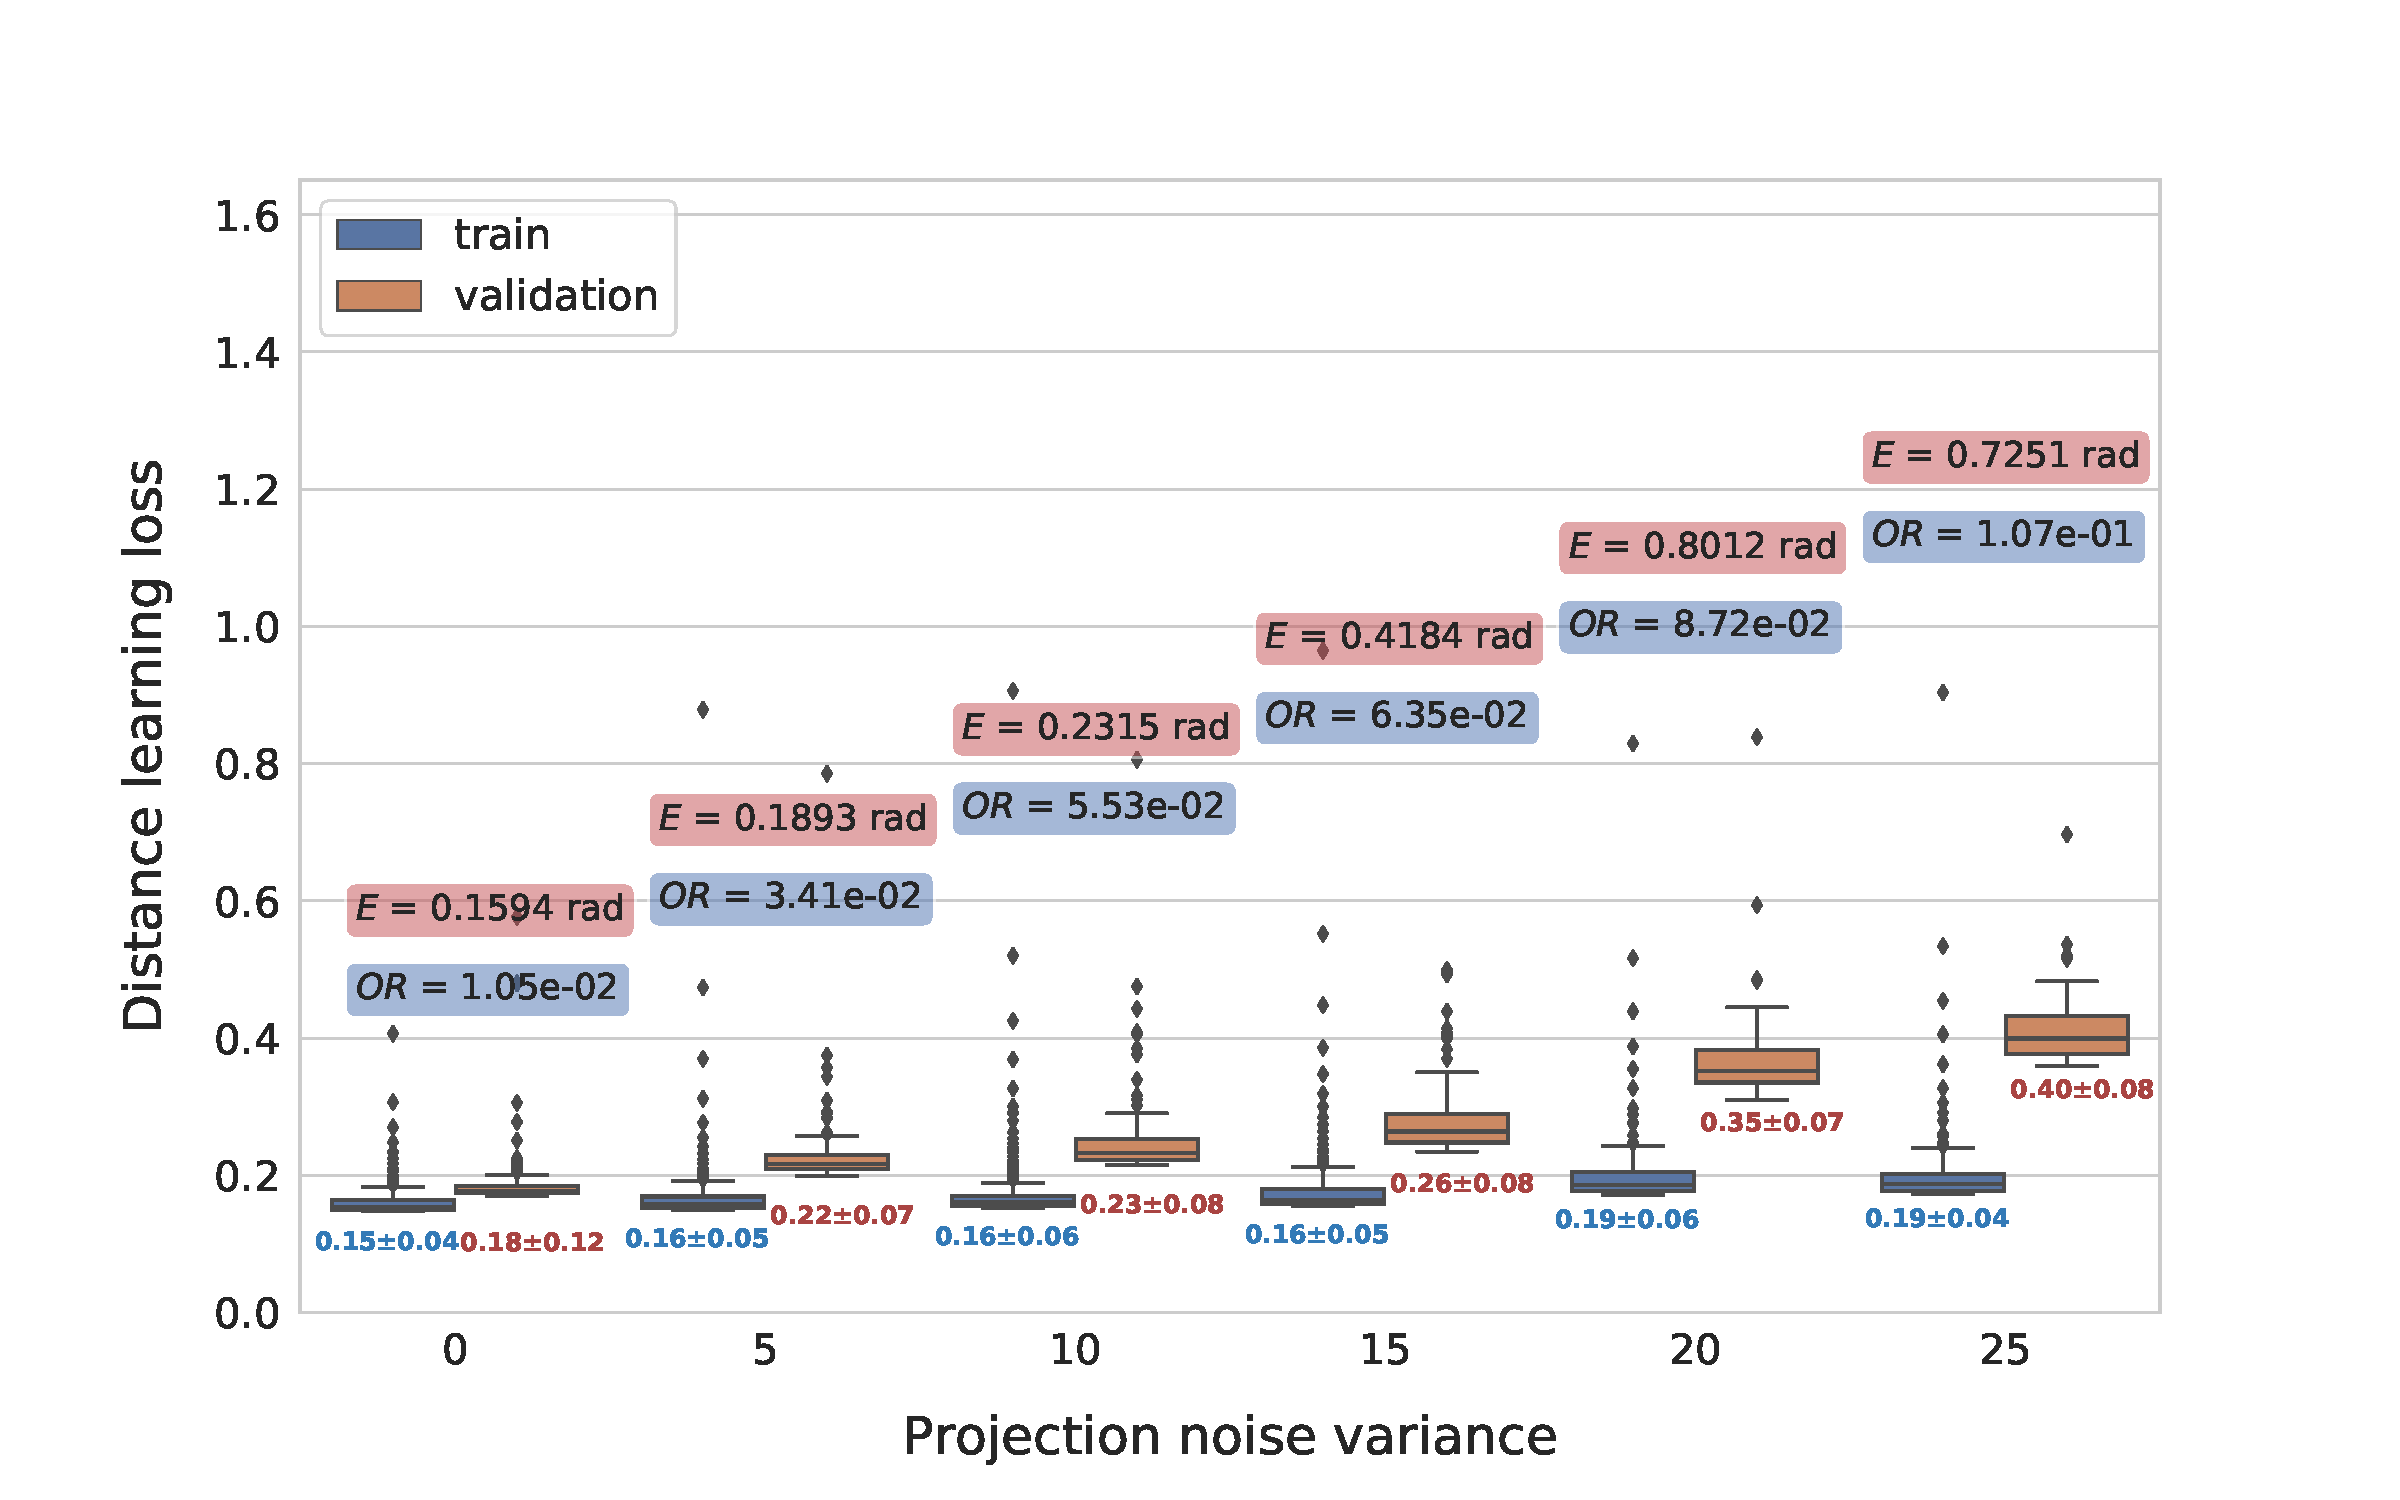
\includegraphics[width=\linewidth]{figures/de_noises_nums}
        \caption{%
            Learning from noisy projections $\{ \mathbf{P}_{\bth_i} \mathbf{x} + \mathbf{n} \}$, with white noise $\mathbf{n} \sim \mathcal{N}(0, \sigma^2\mathbf{I})$ of increasing variance $\sigma^2$.
            Learning is harder as projections get noisier, because noise invariance is not built into the architecture of $\mathcal{G}_w$.
        }\label{fig:results:distance-estimation:noise}
    \end{subfigure}
    \caption{%
        Sensitivity of distance learning to perturbations in the projections of \texttt{5j0n}.
        The box plots show the distance learning loss $L_\text{DE}$~\eqnref{distance-learning} (the distribution is taken over epochs).
        % per epoch on the training and validation sets.
        %\mdeff{Numbers are per pair or per batch of 256 pairs?}
        Boxes show the orientation recovery loss $L_\text{OR}$~\eqnref{orientation-recovery} and error $E_\text{OR}$~\eqnref{orientation-recovery-error}.
    }\label{fig:results:distance-estimation}
\end{figure}

%%%%%%%%%%%%%%%%%%%%%%%%%%%%%%%%%%%%%%%%%%%%%%%%%%%%%%%%%%%%%%%%%%%%%%%%%%%%%%%%%%%%%%%
%%%%%%%%%%%%%%%%%%%%%%%%%%%%%%%%%%%%%%%%%%%%%%%%%%%%%%%%%%%%%%%%%%%%%%%%%%%%%%%%%%%%%%%

\subsection{Orientation recovery and reconstruction of density maps}\label{sec:results:orientation-recovery:reconstruction}

\mdeff{True orientations $\rightarrow$ ground-truth orientations?}
\todo{Insist that reconstructions are only shown to evaluate the recovered orientations (done with ASTRA, not a SOTA iterative method), and that's why we don't reconstruct from noisy projections.}

As a proof-of-concept, we attempted to solve the full inverse problem posed by \eqnref{imaging-model}, \textit{i.e.}, to reconstruct the density maps $\widehat{\x}$ from sets of projections $\{ \p_i \}$ and their orientations $\{ \widehat{q_i} \}$ recovered through the proposed pipeline.
It is worth noting that, at this stage of development, we only trained the SiameseNN on projections originating from the protein we were attempting to reconstruct. This is obviously a very specific experimental case that only partially shines light on the applicability of the method in real situations; this is discussed in Section~\ref{sec:discussion}.

\figref{5j0n-noise0-orientation-recovery} shows the recovery of orientations from distances that were estimated from noiseless projections of \texttt{5j0n}.
A mean error of $E_\text{OR} \approx 0.16$ radians ($\approx 9\degree$) in the recovered orientations led to the reconstruction shown in \figref{5j0n-noise0-reconstruction-recovered}, to be compared to the reconstruction from true orientations shown in \figref{5j0n-noise0-reconstruction-true}.

As predicted by our other experiments, corrupting the projections with a higher level of noise ($\sigma^2=16$) negatively impacts the quality of the orientation recovery (\figref{5j0n-noise16-orientation-recovery}); the obtained mean error is then $E_\text{OR} \approx 0.42$ radians ($\approx 24\degree$).
Unsurprisingly, this leads to a reconstruction with lower resolution, as shown in \figref{5j0n-noise16-reconstruction-recovered}.
\todo{Note that part of this decrease in resolution originates from reconstructing with degraded projections, as the same effect is observed with the reconstruction obtained from true orientations (Figure ??).}
\mdeff{Not true anymore as we don't reconstruct from noisy projections.}

Finally, \figref{5a1a-noise0-orientation-recovery} shows the recovery of orientations from the noiseless projections of \texttt{5a1a}.
A mean error of $E_\text{OR} \approx 0.19$ radians ($\approx 11\degree$) in the recovered orientations led to the reconstruction shown in \figref{5j0n-noise0-reconstruction-recovered}, to be compared to \figref{5j0n-noise0-reconstruction-true}.
Orientation recovery is slightly more difficult for this protein as distance estimation is more difficult (\secref{results:distance-estimation:learned}).

To further illustrate the impact of errors in the recovered orientations, we compared the density maps reconstructed from the recovered orientations $\{ \widehat{q_i} \}$ to that reconstructed from the true orientations $\{ q_i \}$. All density maps were reconstructed using the ASTRA toolbox. The results are displayed in~\figref{reconstructions}, \lau{and show that an accurate first volume can be reconstructed from the projections whose orientations have been recovered through our method.}
%\lau{\textit{We don't need to keep what follows anymore, right?} The rationale behind not comparing directly with the original ground-truth (\figref{pdb-proteins}) is that the robustness of the reconstruction method can impact the quality of the reconstruction when only few projections are considered, which was the case here (only $1,650$ projections).}

In conclusion, the more accurate the estimation of the pairwise distances, the higher the quality of the orientation recovery, which leads to reconstructions with a higher resolution. %This indicates that the quality of the reconstruction would substantially improve should a more powerful SiameseNN  be trained on more data for distance estimation (and a more robust method used for reconstruction).

\begin{figure}[t]
    \centering
    \begin{subfigure}[b]{0.26\linewidth}
        \centering
        %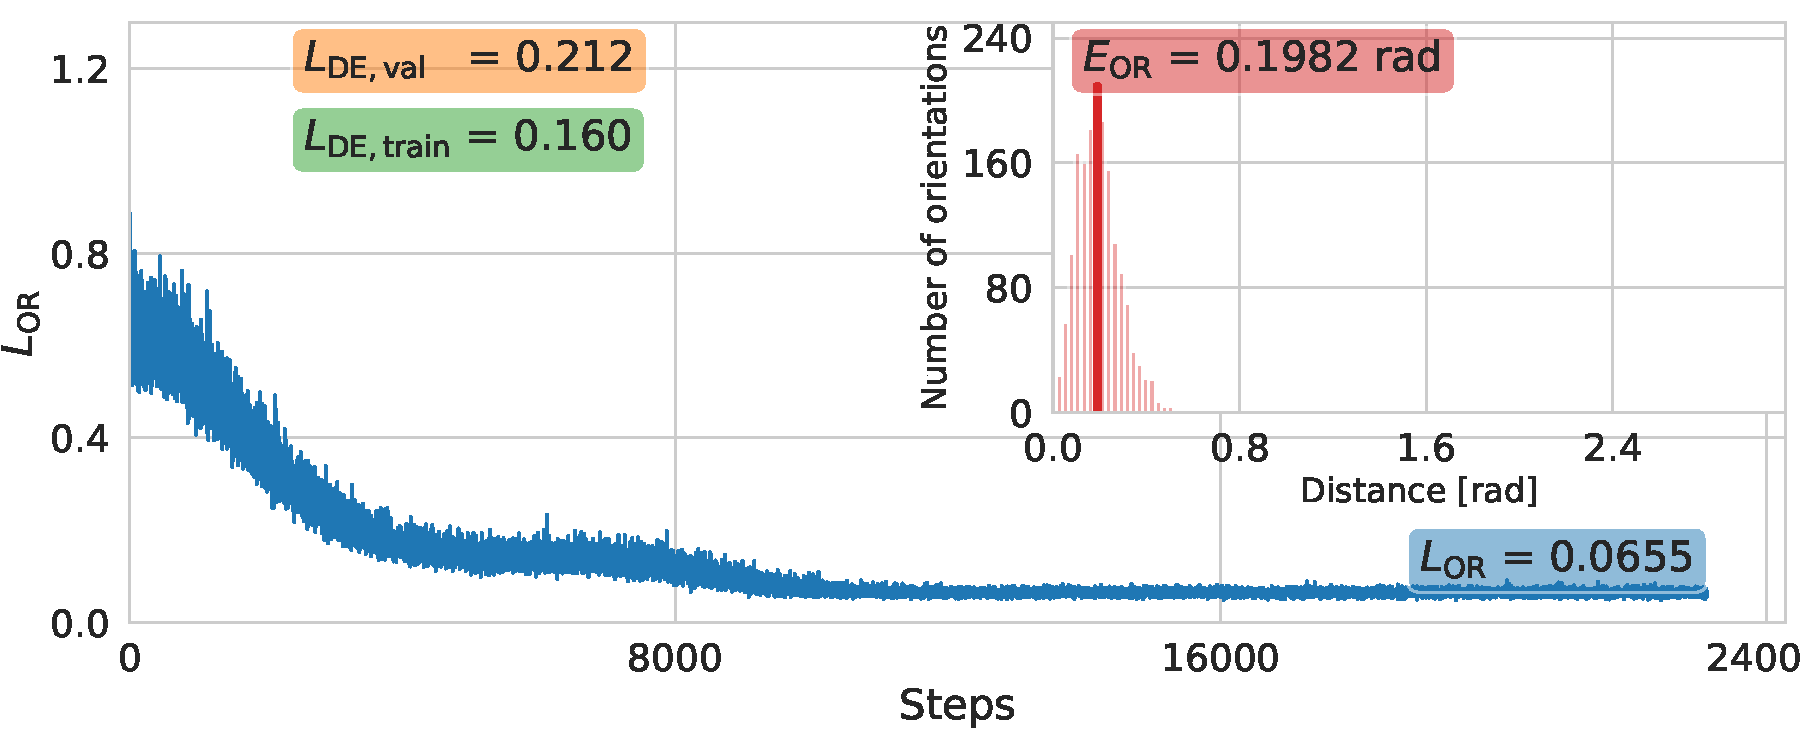
\includegraphics[height=3cm]{figures/5j0n_ar_aa_fullcvg_uniform2}
        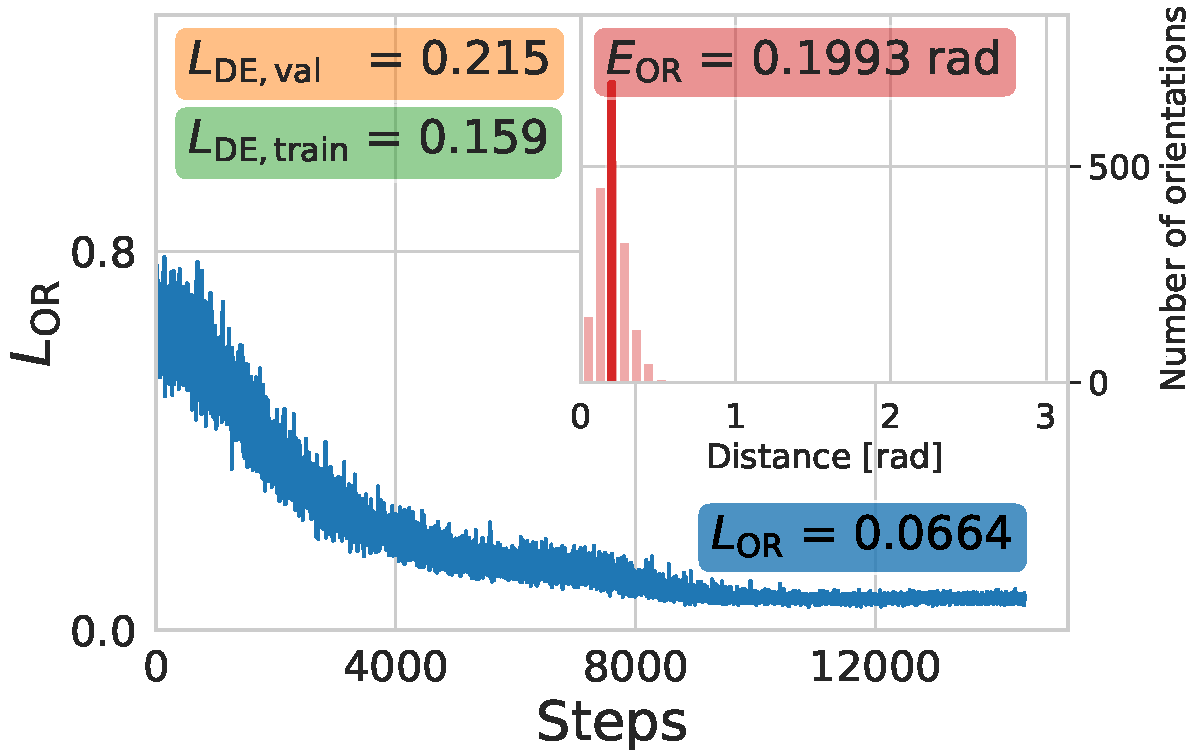
\includegraphics[height=2.4cm]{figures/5j0n_fullcvg_uniformS2_noise0_ar_aa.pdf}
        \caption{Noiseless projections of \texttt{5j0n}.}%
        \label{fig:5j0n-noise0-orientation-recovery}
    \end{subfigure}
    \hfill
    \begin{subfigure}[b]{0.23\linewidth}
        \centering
        %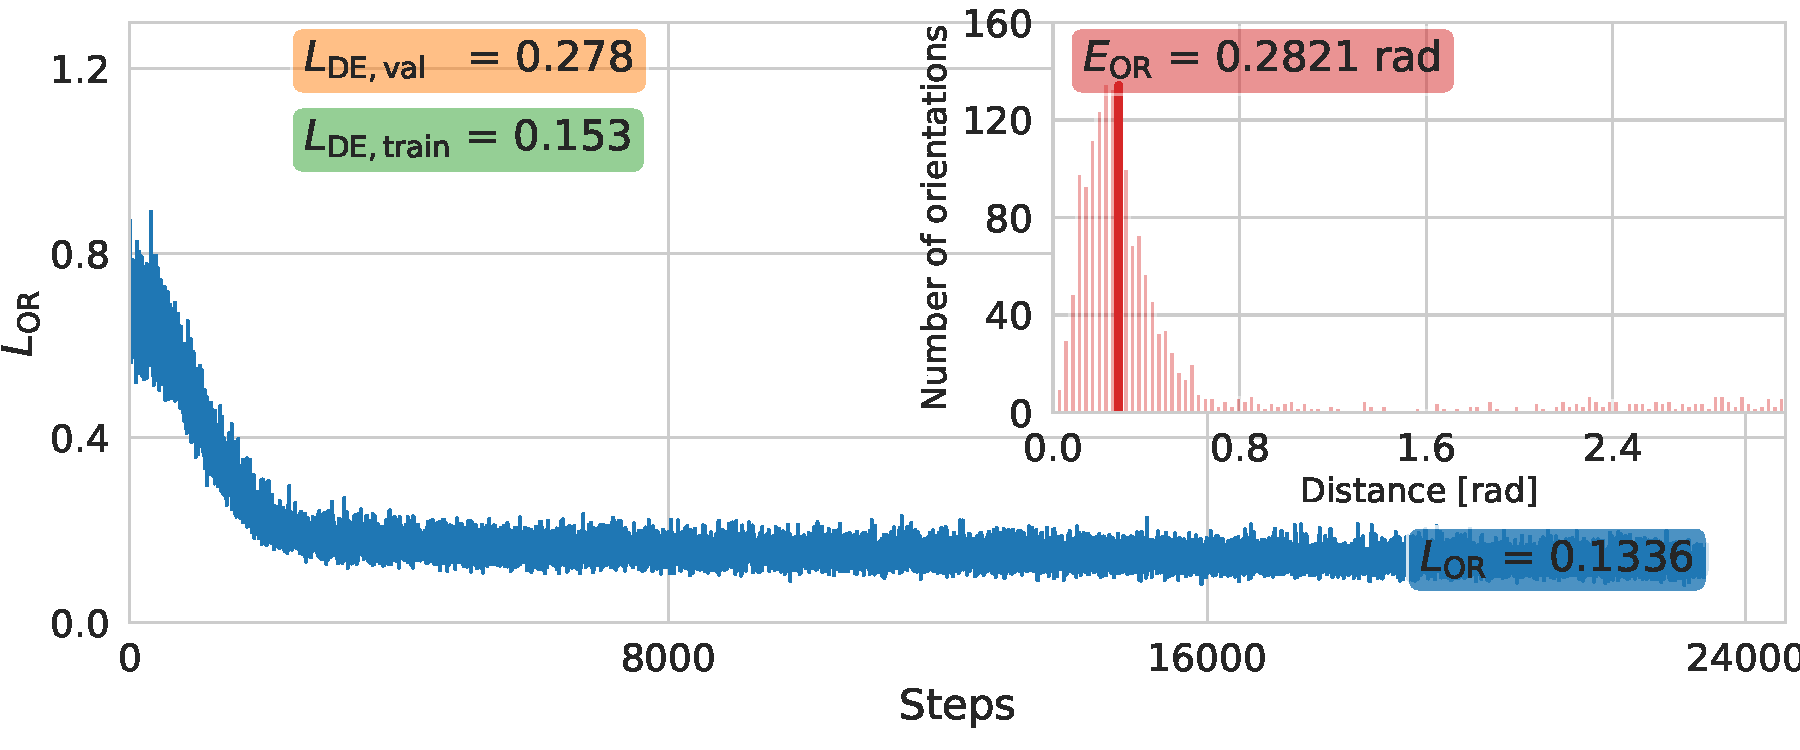
\includegraphics[height=3cm]{figures/5j0n_fullcov_noise16_ar_aa}
        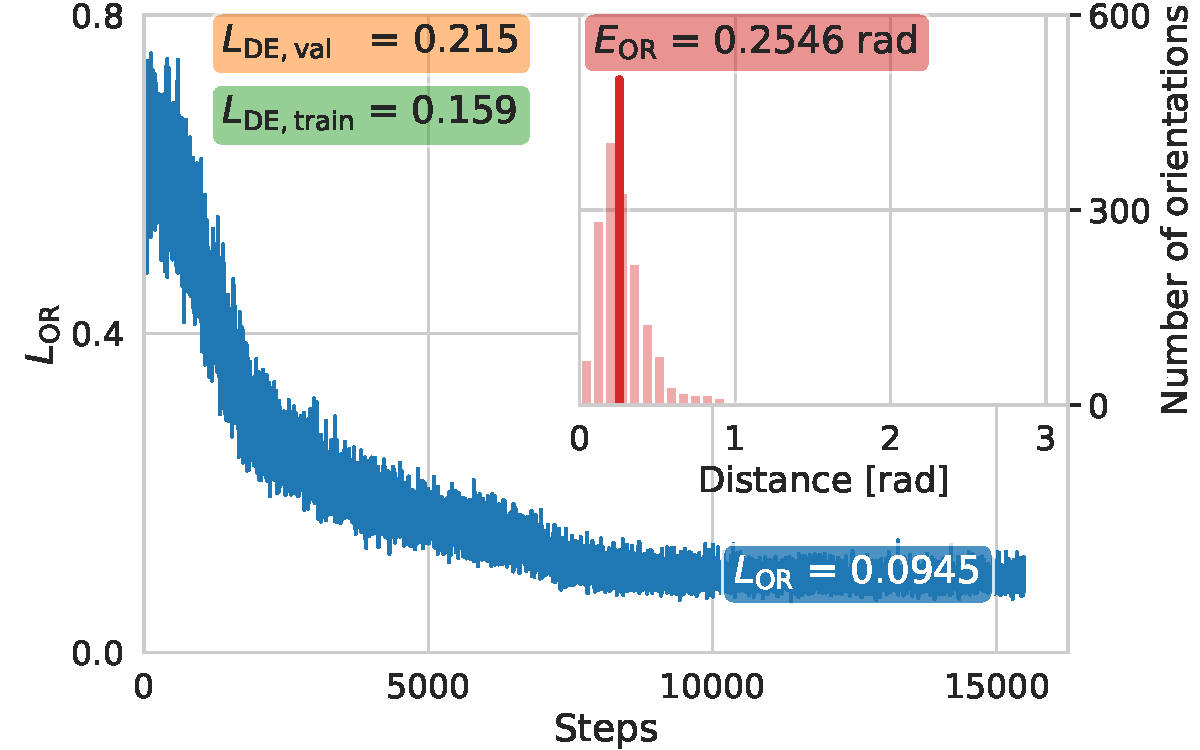
\includegraphics[height=2.4cm]{figures/5j0n_fullcvg_uniformS2_noise16_ar_aa.pdf}
        \caption{Noisy projections of \texttt{5j0n}.}%
        \label{fig:5j0n-noise16-orientation-recovery}
    \end{subfigure}
    \hfill
    \begin{subfigure}[b]{0.26\linewidth}
        \centering
        %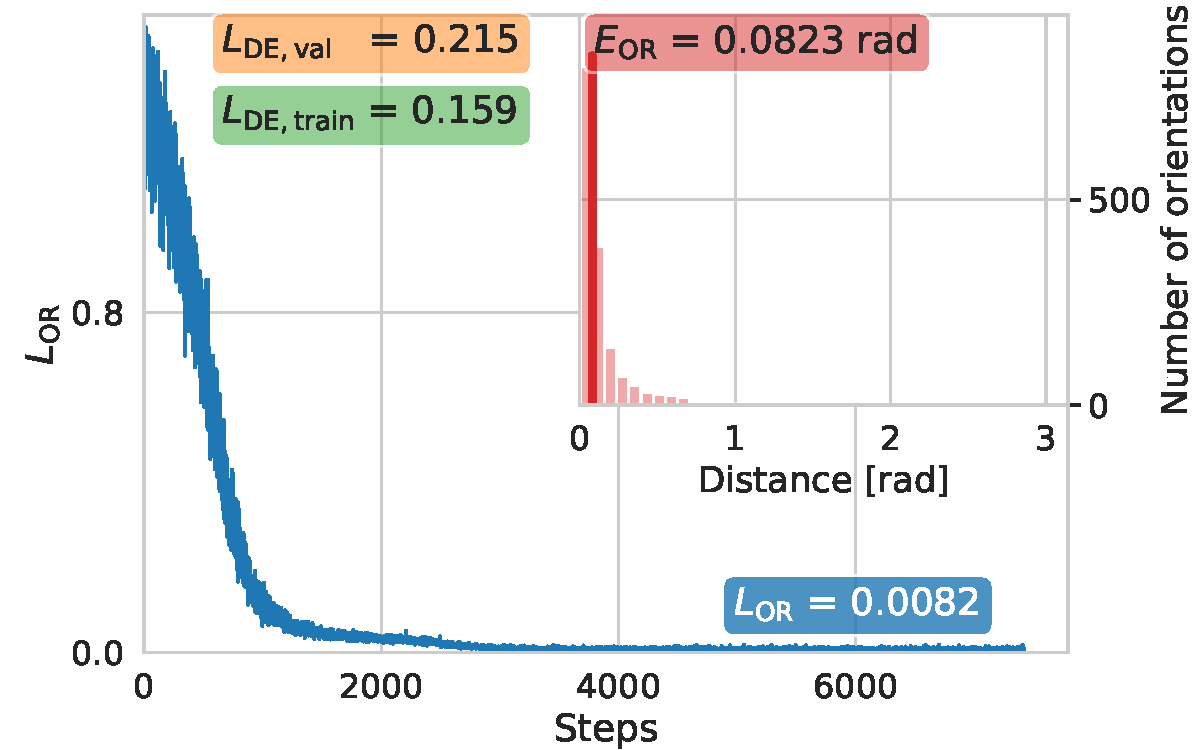
\includegraphics[width=\linewidth]{figures/5a1a_quartercov_uniformS2_noise0_halfInplane_ar_aa.pdf}
        % 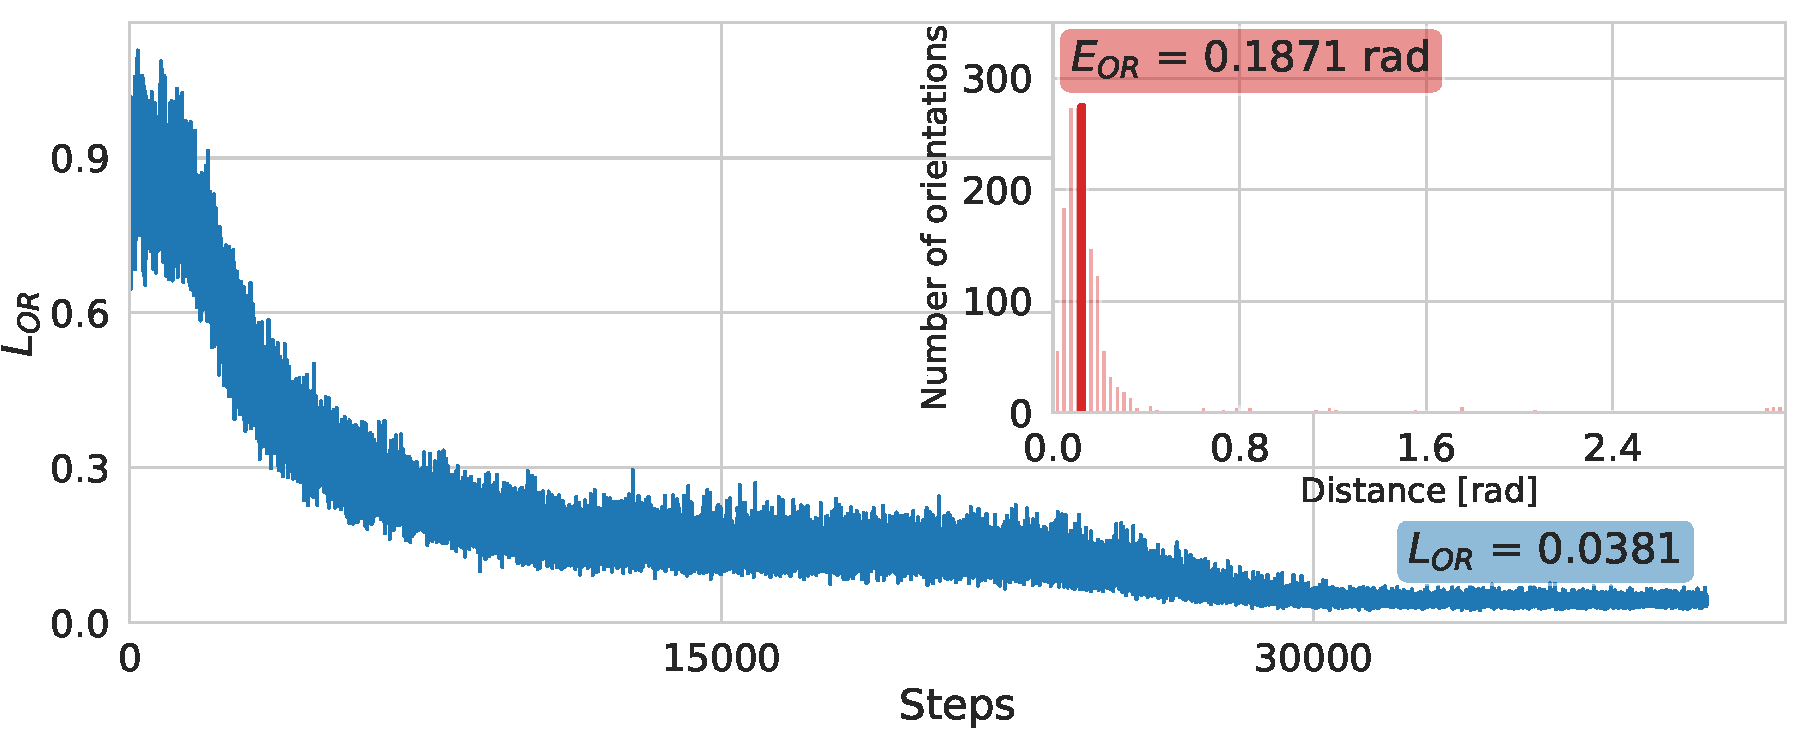
\includegraphics[width=\linewidth]{figures/5a1a_noise0_ar_aa.pdf}
        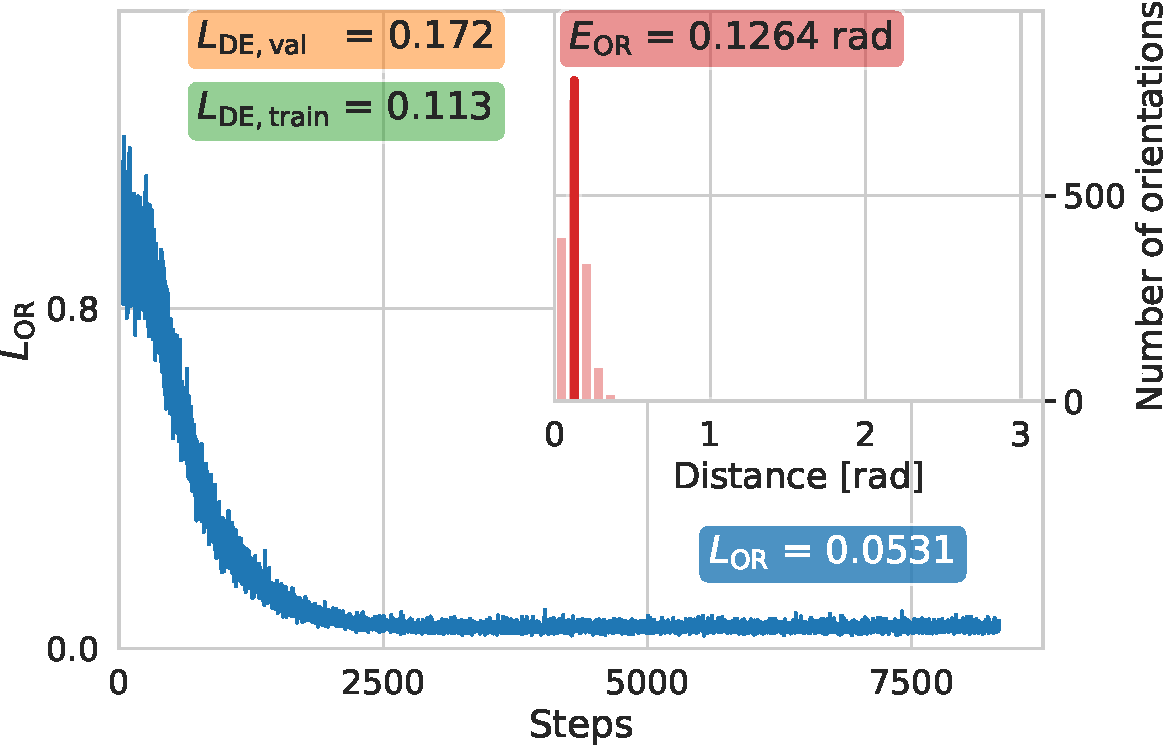
\includegraphics[height=2.4cm]{figures/5a1a_quartercov_uniformS2_noise0_LAST_ar_aa.pdf}
        \caption{Noiseless projections of \texttt{5a1a}.
        }%
        \label{fig:5a1a-noise0-orientation-recovery}
    \end{subfigure}
    \begin{subfigure}[b]{0.23\linewidth}
        \centering
        %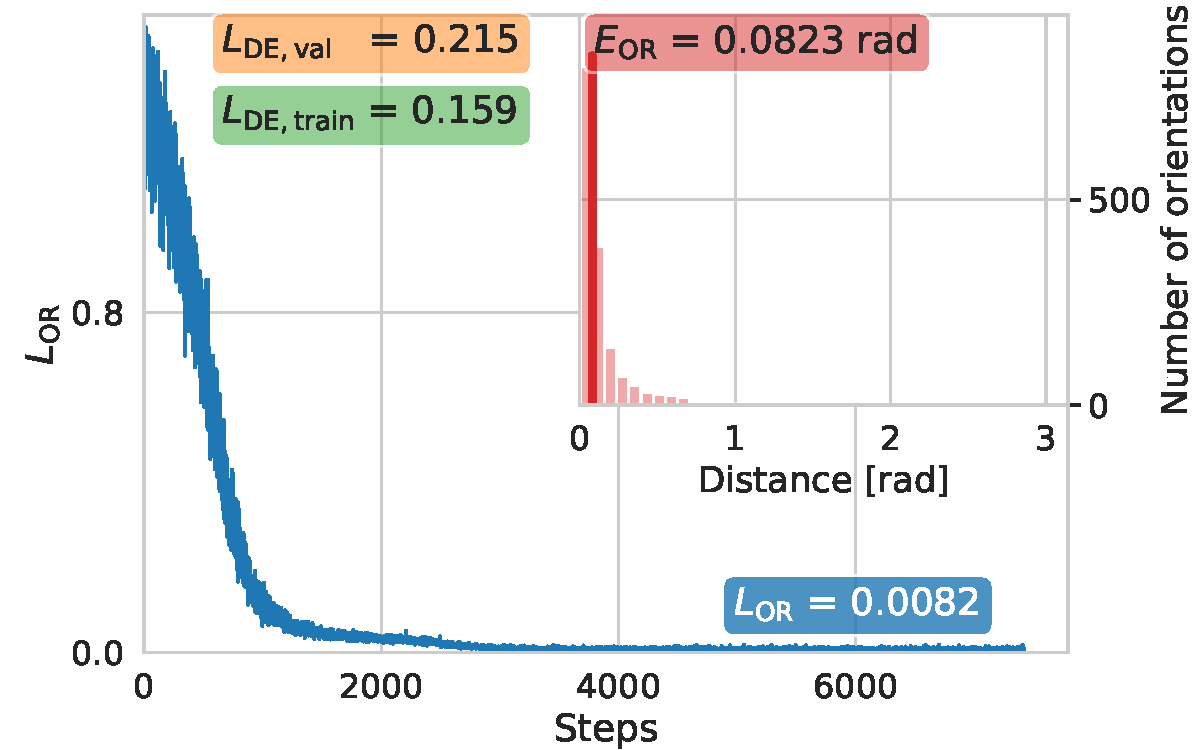
\includegraphics[width=\linewidth]{figures/5a1a_quartercov_uniformS2_noise0_halfInplane_ar_aa.pdf}
        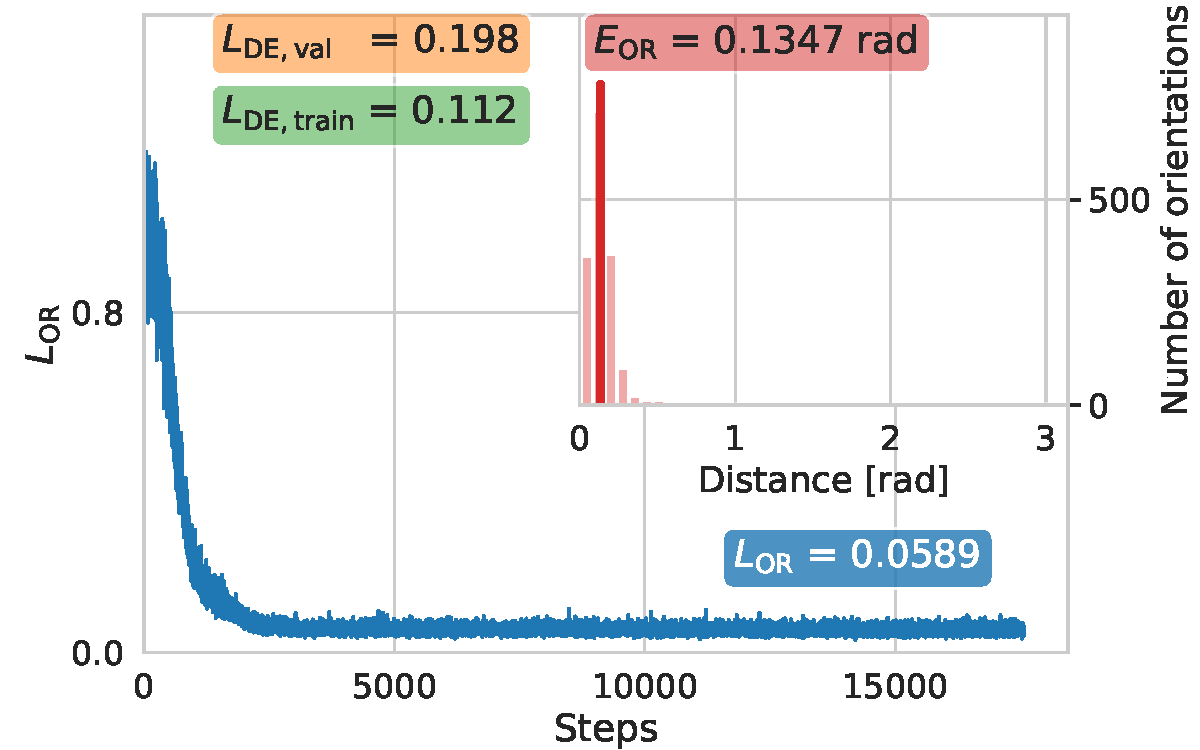
\includegraphics[height=2.4cm]{figures/5a1a_quartercov_uniformS2_noise16_LAST_ar_aa.pdf}
        \caption{Noisy projections of \texttt{5a1a}.
        }%
        \label{fig:5a1a-noise16-orientation-recovery}
    \end{subfigure}
    \hfill
    % \begin{subfigure}[b]{0.22\linewidth}
    %     \centering
    %     %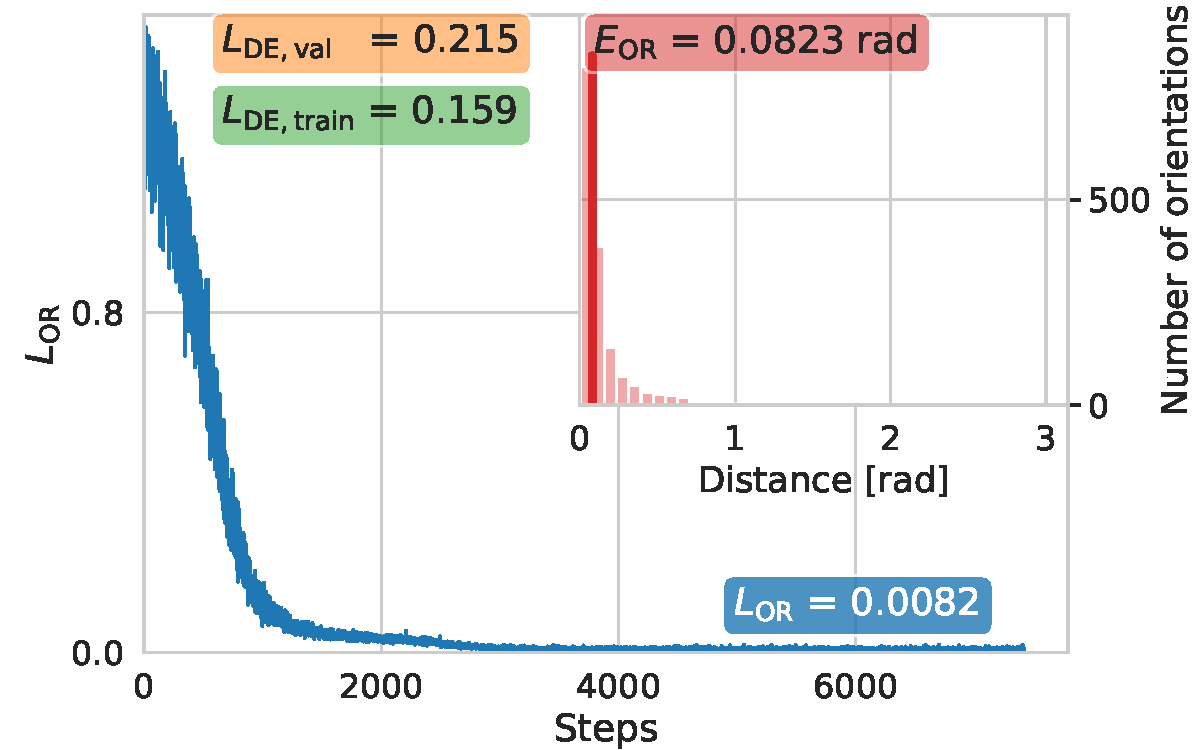
\includegraphics[width=\linewidth]{figures/5a1a_quartercov_uniformS2_noise0_halfInplane_ar_aa.pdf}
    %     %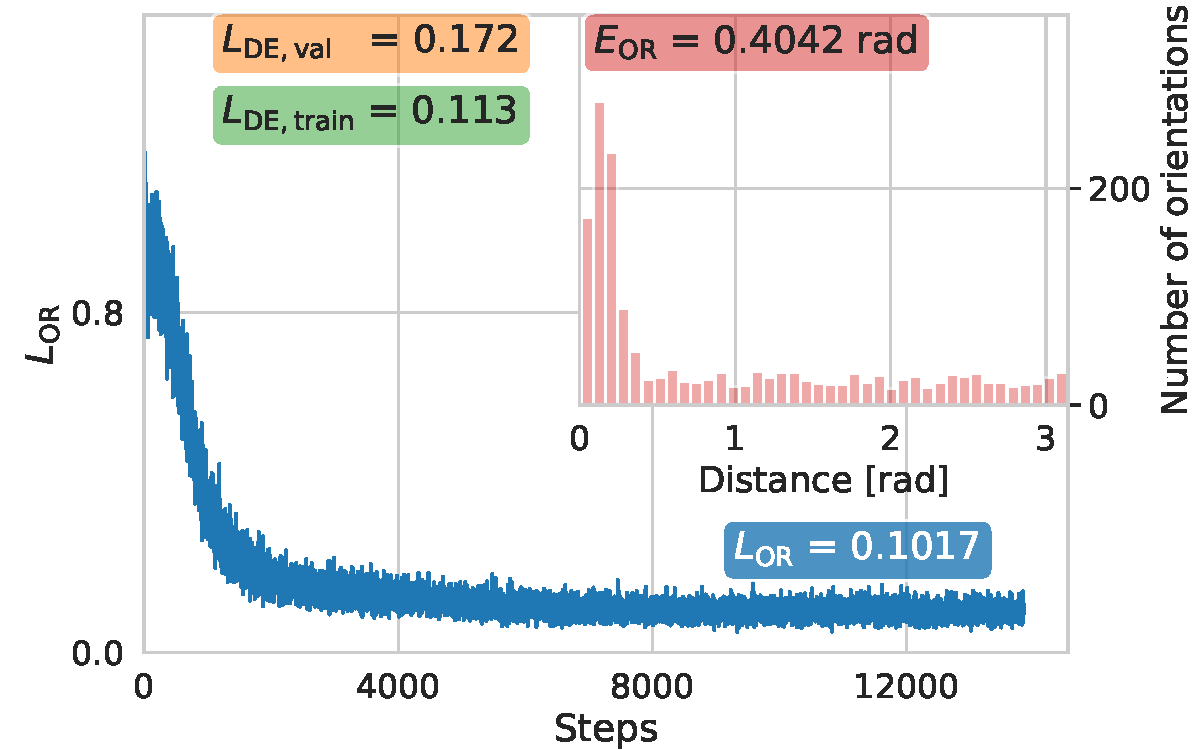
\includegraphics[width=\linewidth]{figures/5a1a_quartercov_uniformS2_noise0_ar_aa.pdf}
    %     %\caption{Noiseless projections of \texttt{5a1a}.}%
    %     \label{fig:5a1a-noise0-orientation-recovery-quarter-full}
    % \end{subfigure}
    \caption{%
        % Our pipeline.
        Distance learning and orientation recovery from estimated distances.
        The green and orange boxes show $L_\text{DE}$ \eqnref{distance-learning} on the training and validation sets.
        The blue curve shows the evolution of the recovery loss until convergence, with the minimum $L_\text{OR}$ \eqnref{orientation-recovery} highlighted.
        The red histogram shows the errors in the recovered orientations $\{d_q(q_i, \mathbf{T}\widehat{q_i})\}$, with the mean $E_\text{OR}$ \eqnref{orientation-recovery-error} highlighted.
        % Explain columns then rows.
        % The first row~(a,b,c) shows the process for noiseless projections $\p_i = \mathbf{P}_{\bth_i} \x$, where $\x$ comes from \texttt{5j0n}.
        % The second row~(d,e,f) shows the process for noisy projections $\p_i = \mathbf{P}_{\bth_i} \x + \mathbf{n}$, where $\mathbf{n} \sim \mathcal{N}(0, \sigma^2\mathbf{I}), \sigma^2=16$, and $\x$ comes from \texttt{5j0n}.
        % The third row~(g,h,i) shows the process for noiseless projections $\p_i = \mathbf{P}_{\bth_i} \x$, where $\x$ comes from \texttt{5a1a}.
    }
\end{figure}

\begin{figure}[t]
    \begin{subfigure}[b]{0.17\linewidth}
        \centering
        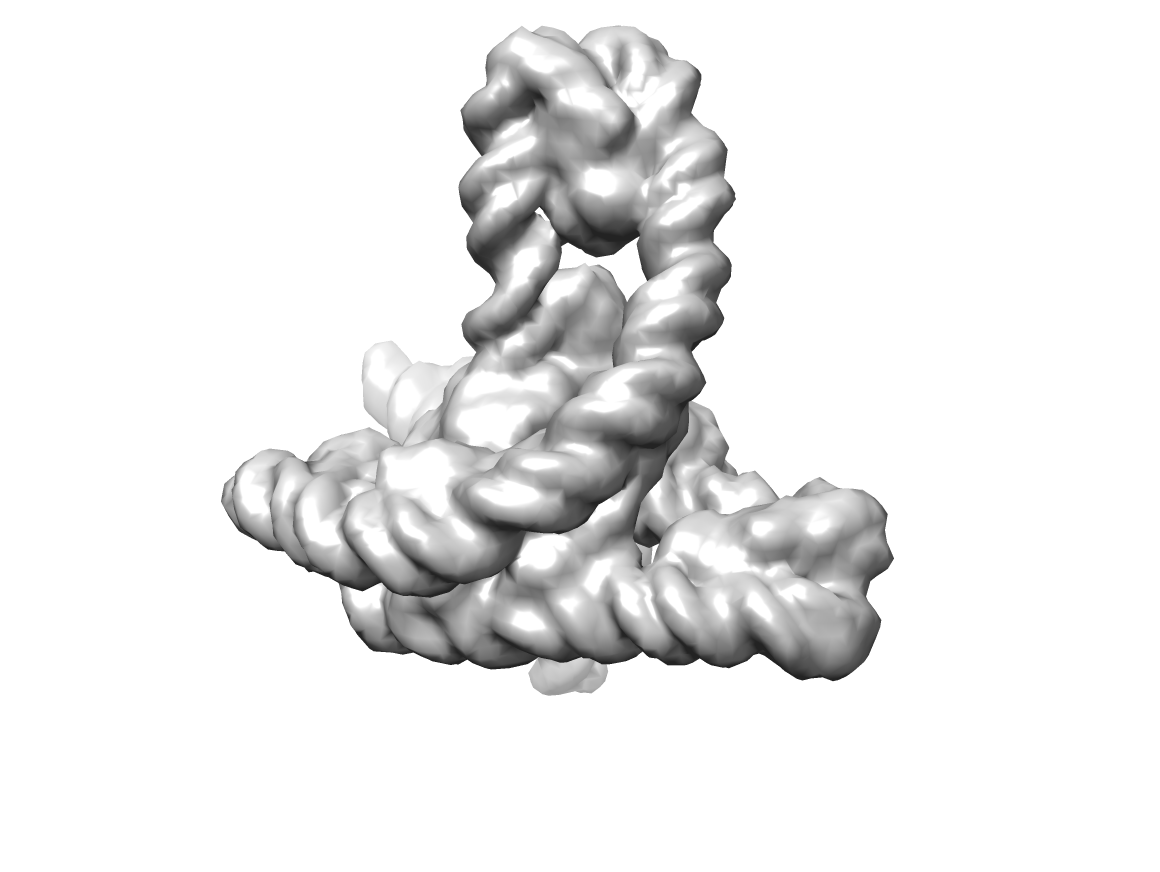
\includegraphics[height=2.5cm]{figures/5j0n_fullcvg_uniformS2_noise0_gt.png}
        \caption{}\label{fig:5j0n-noise0-reconstruction-true}
    \end{subfigure}
    \hfill
    \begin{subfigure}[b]{0.16\linewidth}
        \centering
        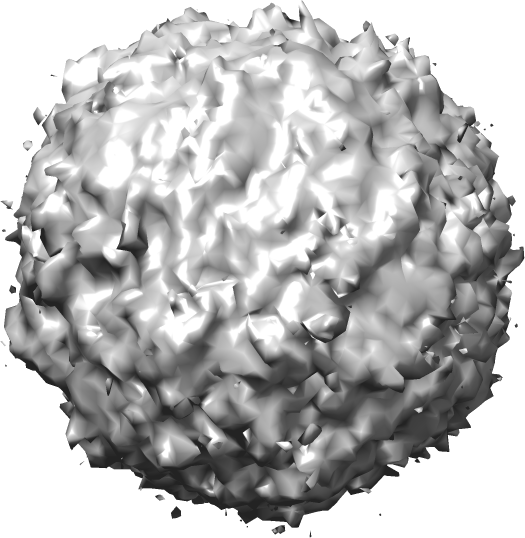
\includegraphics[height=2.5cm]{figures/5j0n_fullcvg_uniformS2_noise0_rand.png}
        \caption{}
    \end{subfigure}
    \hfill
    \begin{subfigure}[b]{0.15\linewidth}
        \centering
        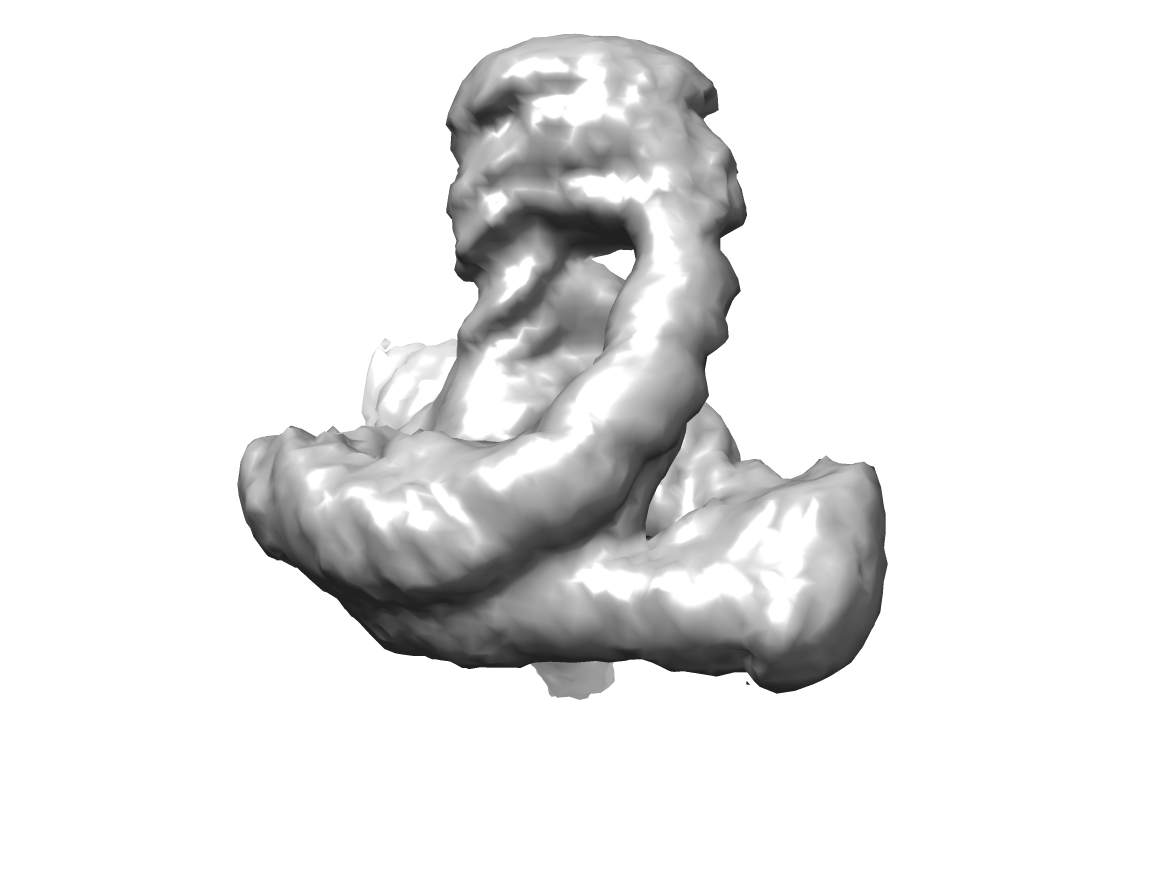
\includegraphics[height=2.5cm]{figures/5j0n_fullcvg_uniformS2_noise0_apr.png}
        \caption{}\label{fig:5j0n-noise0-reconstruction-recovered}
    \end{subfigure}
    \hfill
    \begin{subfigure}[b]{0.15\linewidth}
        \centering
        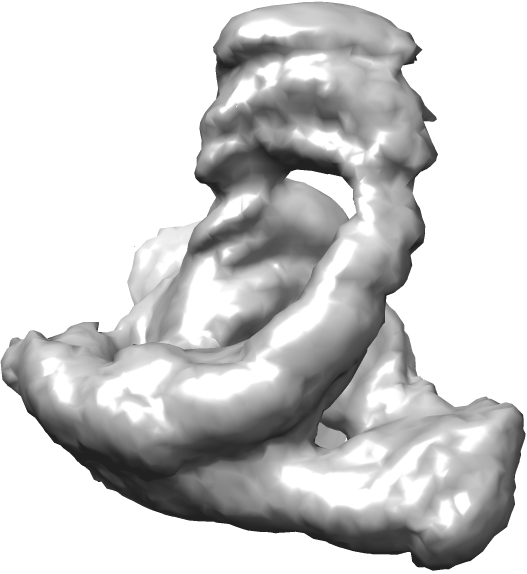
\includegraphics[height=2.5cm]{figures/5j0n_fullcvg_uniformS2_noise16_apr.png}
        \caption{}\label{fig:5j0n-noise16-reconstruction-recovered}
    \end{subfigure}
    \hfill
    \begin{subfigure}[b]{0.30\linewidth}
        \centering
        %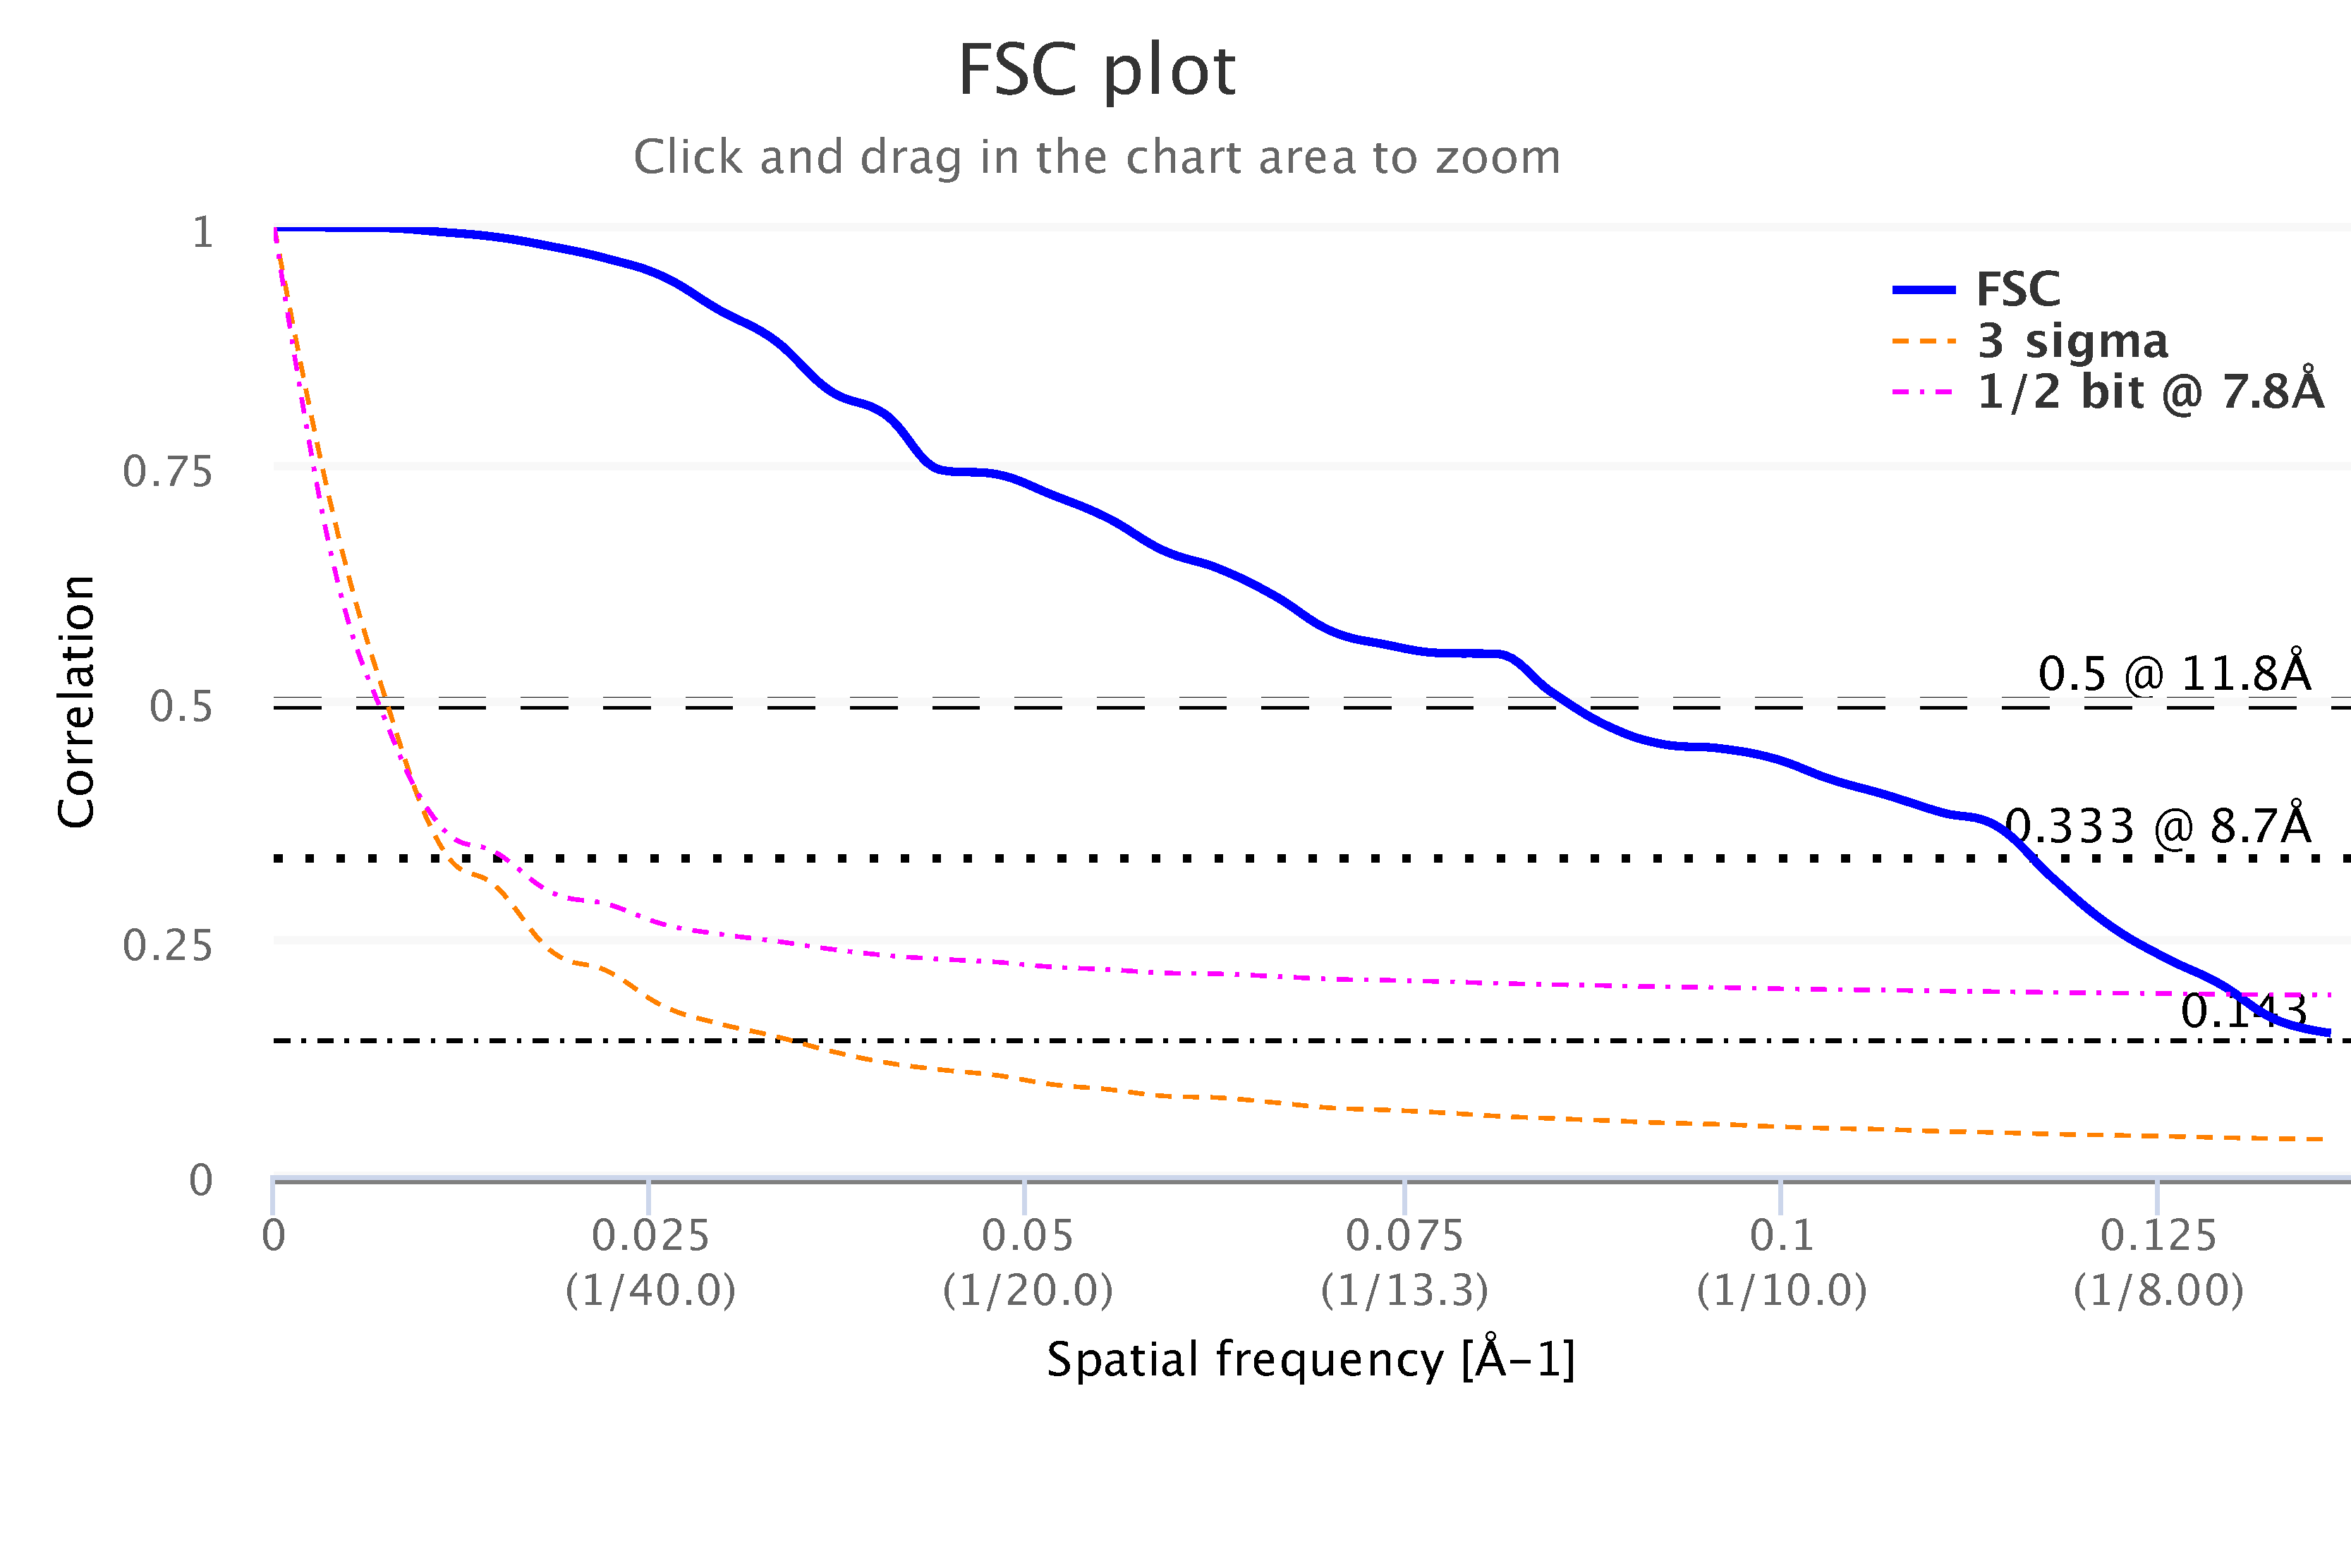
\includegraphics[height=3cm]{figures/FSC_5j0n_fullcvg_uniformS2_noise0_fin_vs_init.pdf}
        %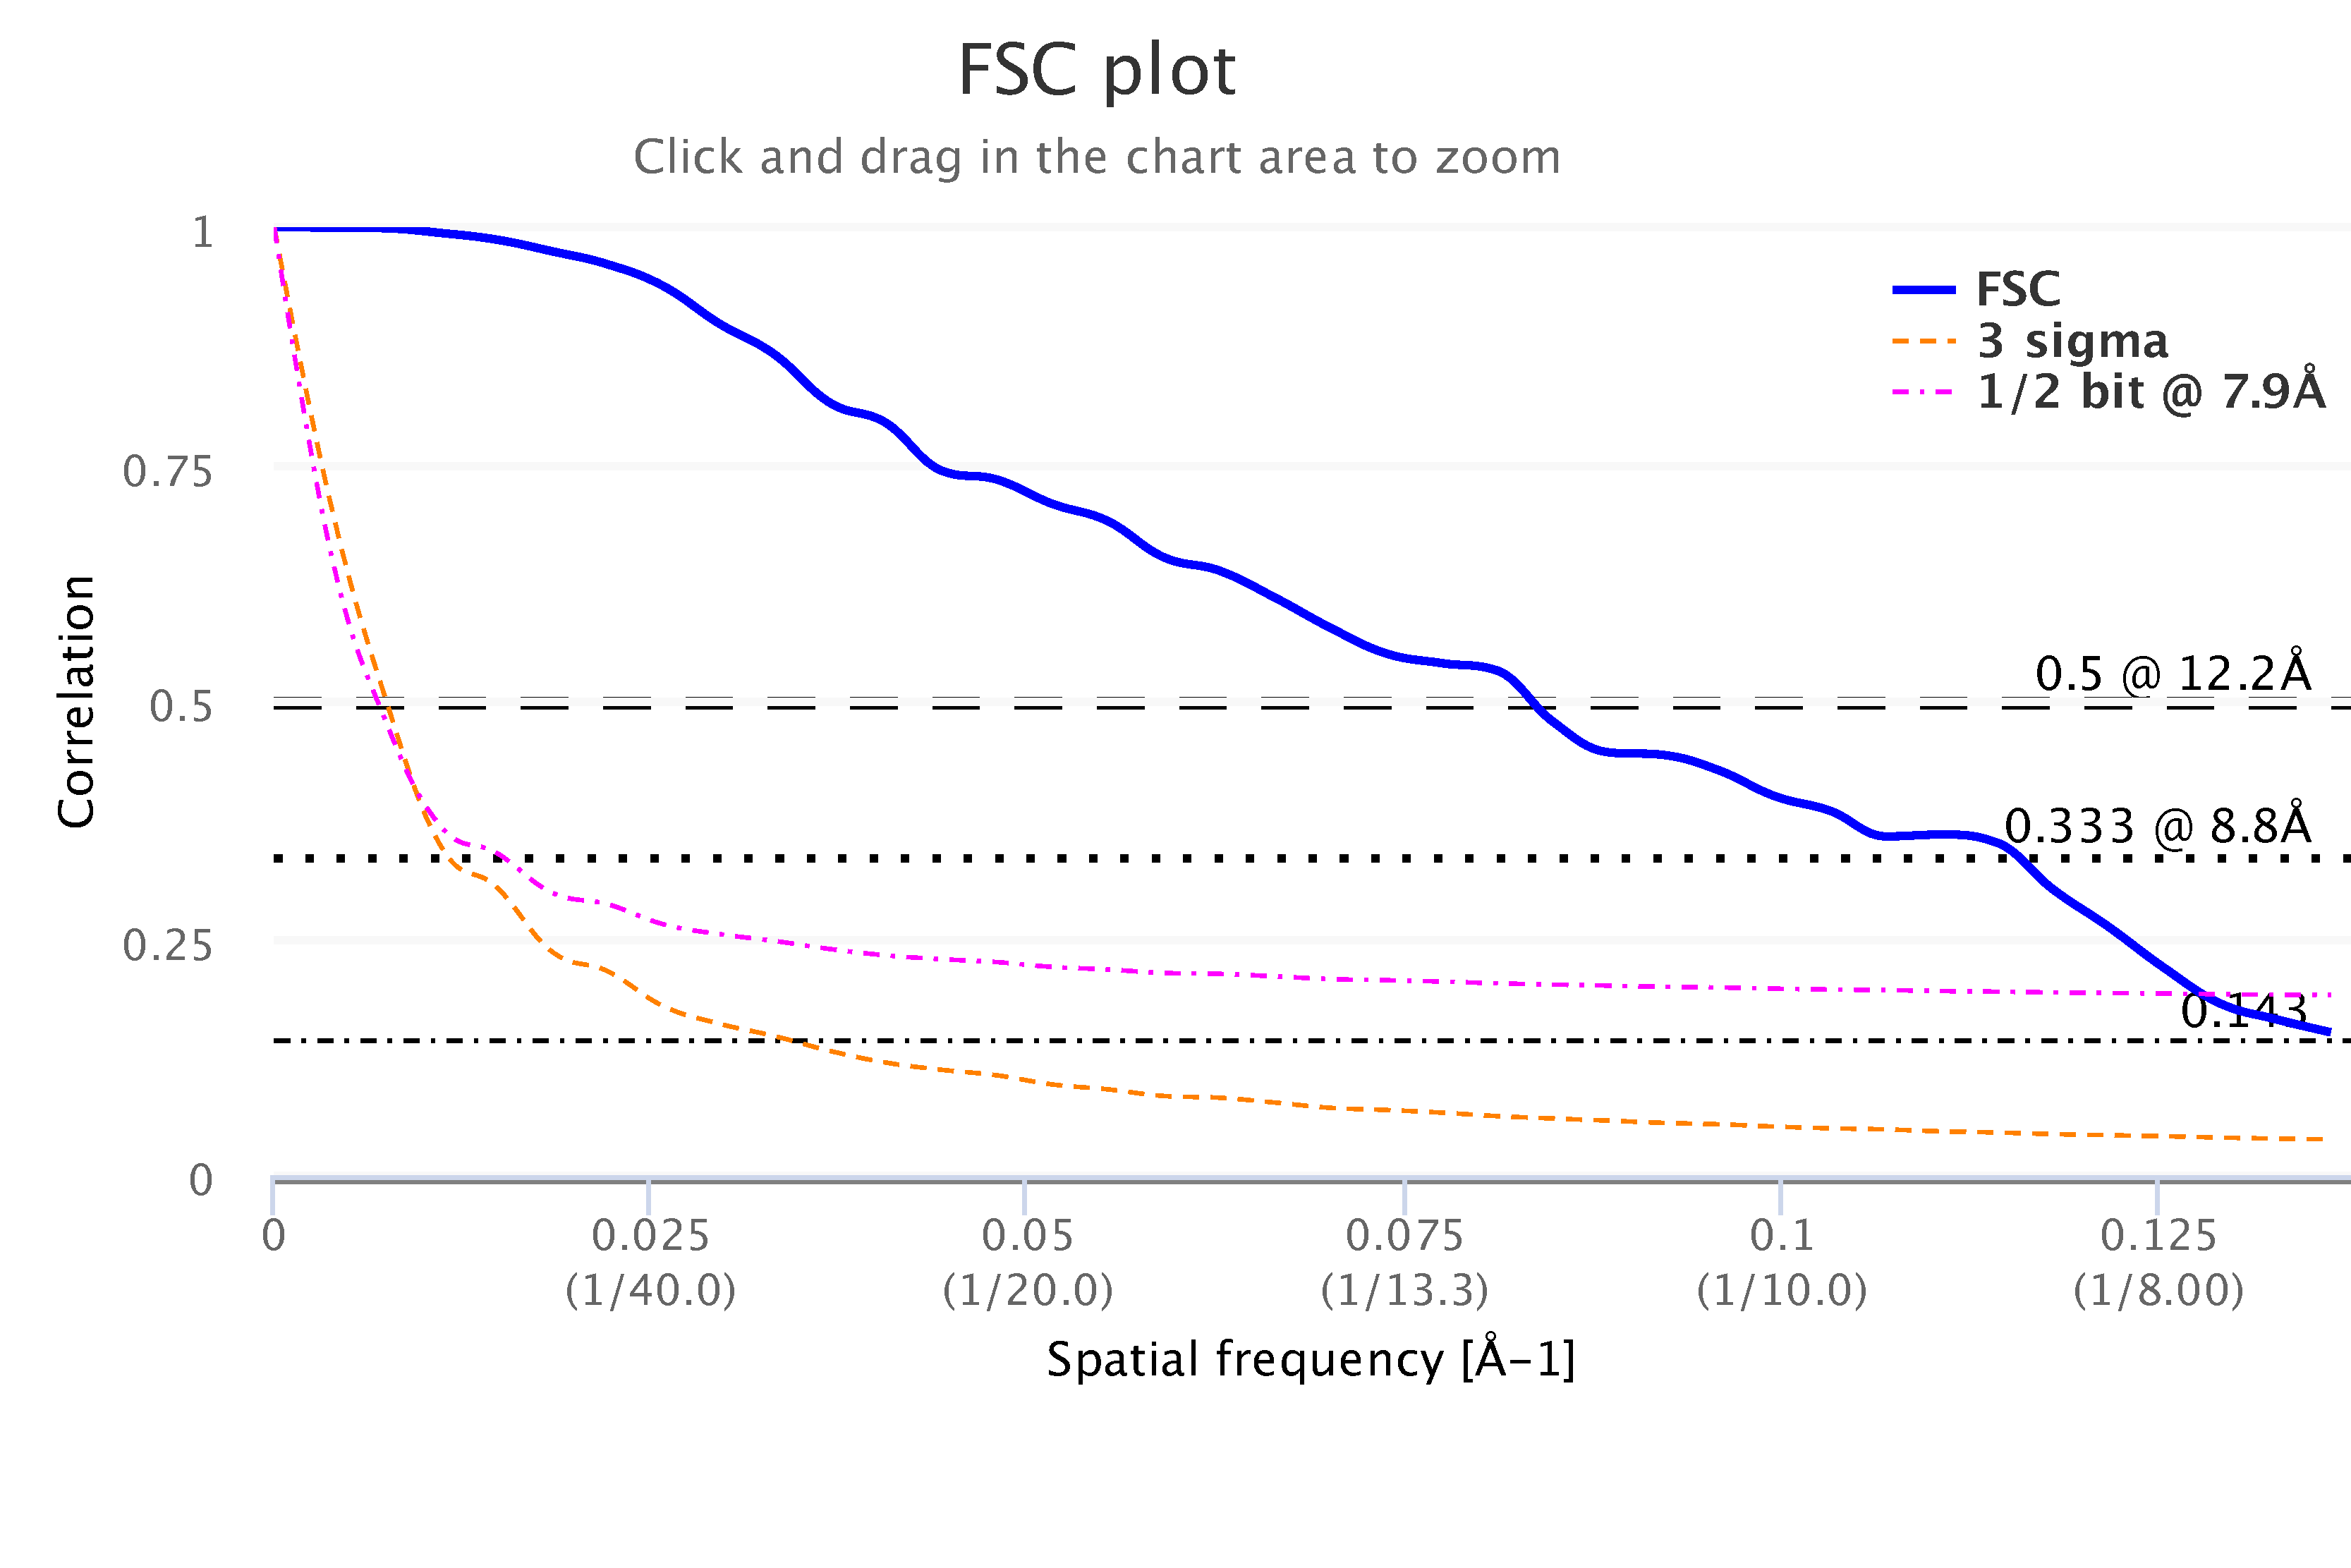
\includegraphics[height=3cm]{figures/5j0n_fullcvg_uniformS2_noise0_FSC_apr_init.pdf}
        %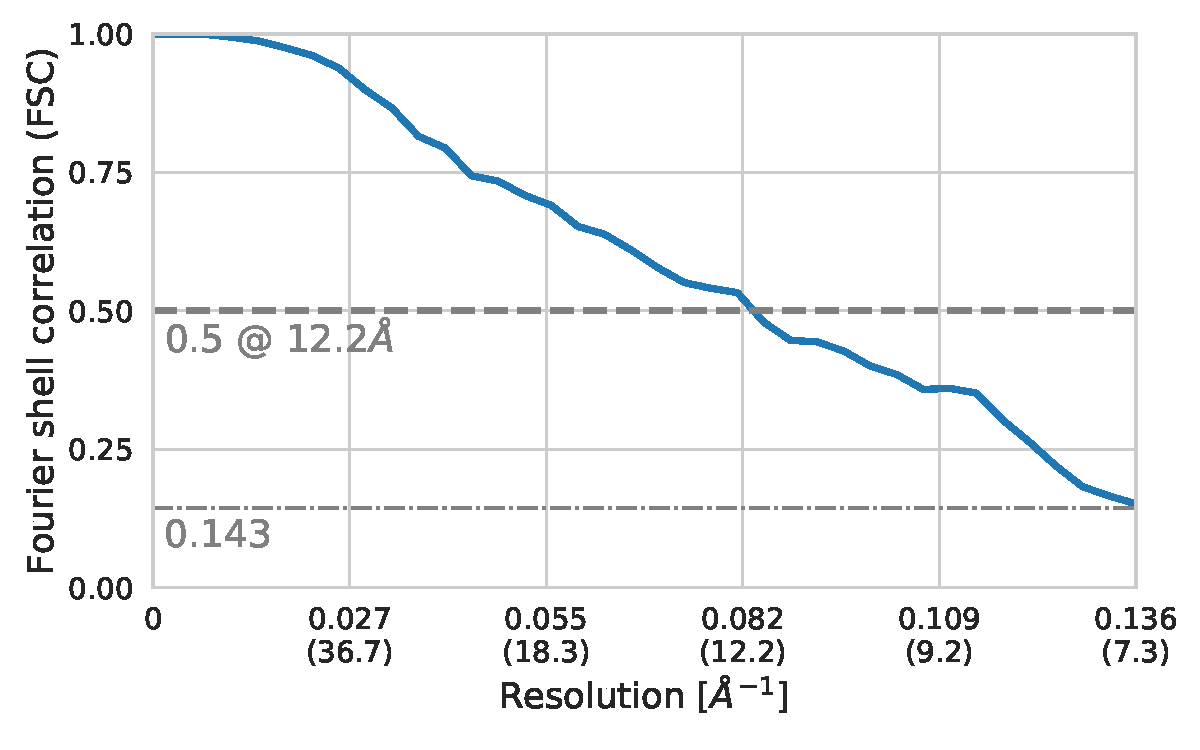
\includegraphics[height=3cm]{figures/5j0n_fullcvg_uniformS2_noise0_FSC_apr_init_customFSC.pdf}
        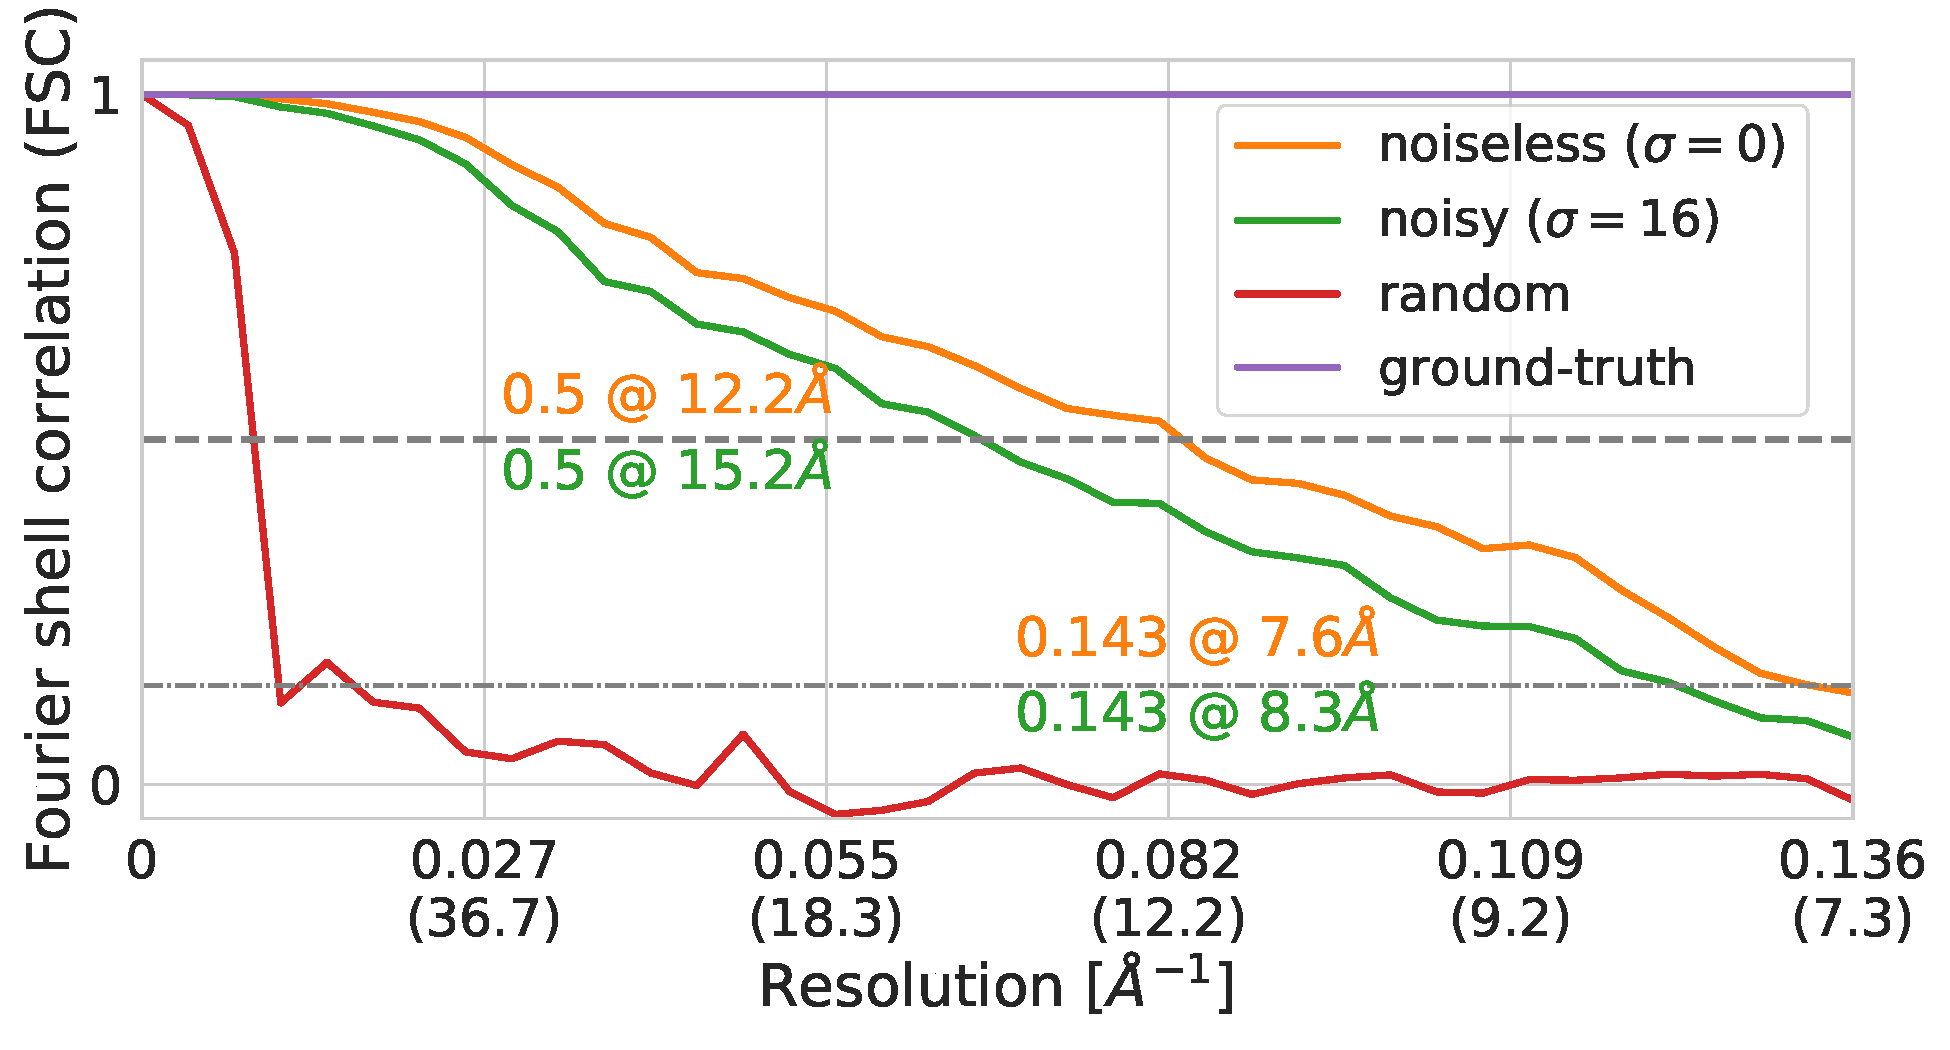
\includegraphics[height=2.5cm]{figures/5j0n_fullcvg_uniformS2_FSC_apr_init_customFSC2.pdf}
        \caption{}
    \end{subfigure}

    \vspace{1em}
    \begin{subfigure}[b]{0.17\linewidth}
        \centering
        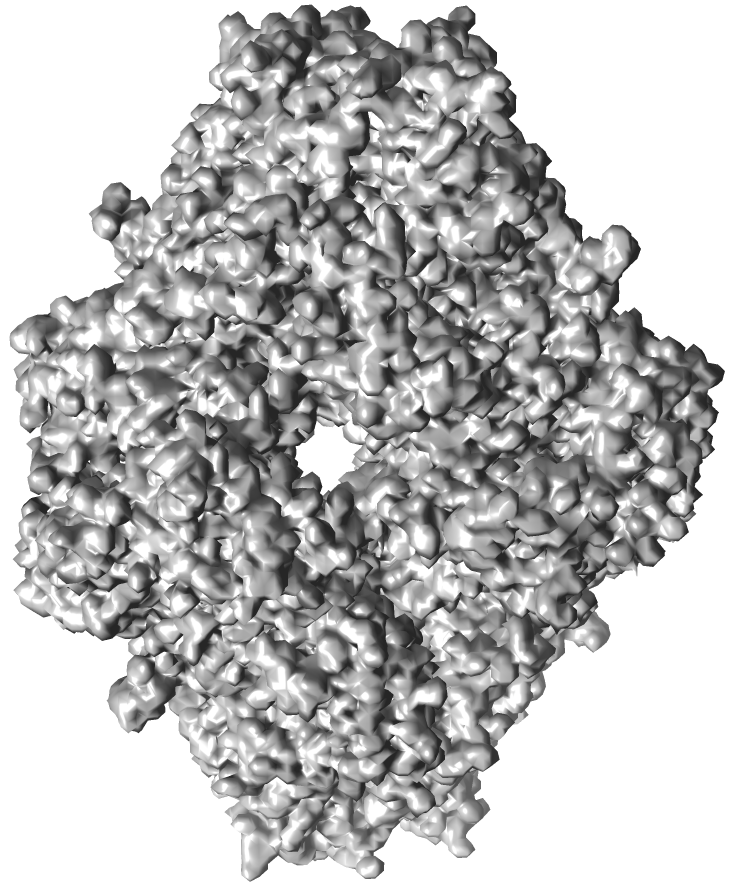
\includegraphics[height=2.5cm]{figures/5a1a_quartercov_uniformS2_noise0_gt_.png}
        \caption{}\label{fig:5a1a-noise0-reconstruction-true}
    \end{subfigure}
    \hfill
    \begin{subfigure}[b]{0.16\linewidth}
        \centering
        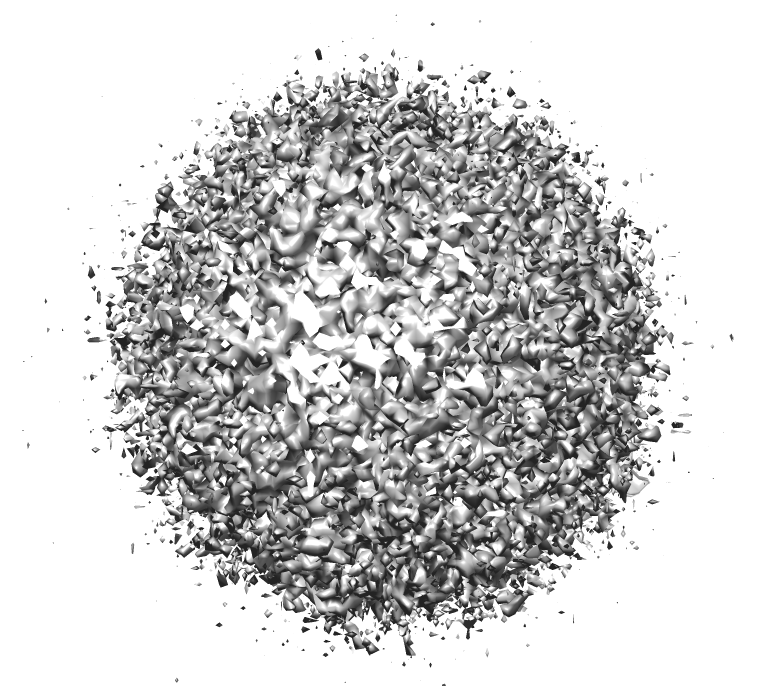
\includegraphics[height=2.5cm]{figures/5a1a_quartercov_uniformS2_noise0_rand.png}
        \caption{}
    \end{subfigure}
    \hfill
    \begin{subfigure}[b]{0.15\linewidth}
        \centering
        %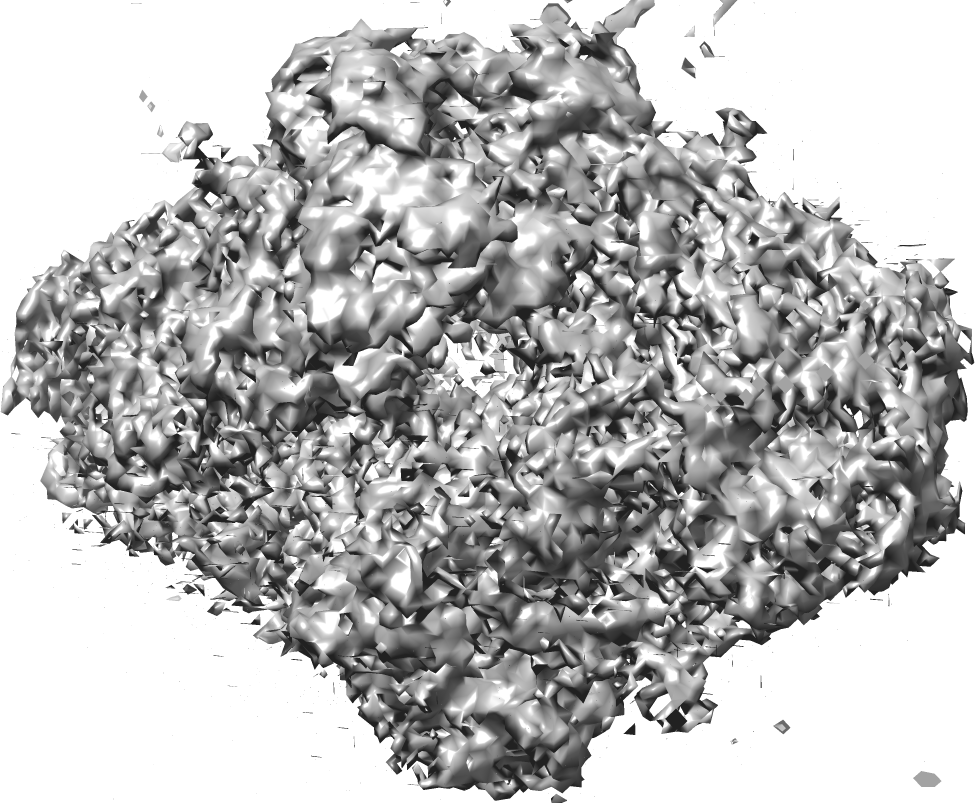
\includegraphics[height=3cm]{figures/r5a1a_quartercov_uniformS2_noise0_halfInplane_apr.png}
        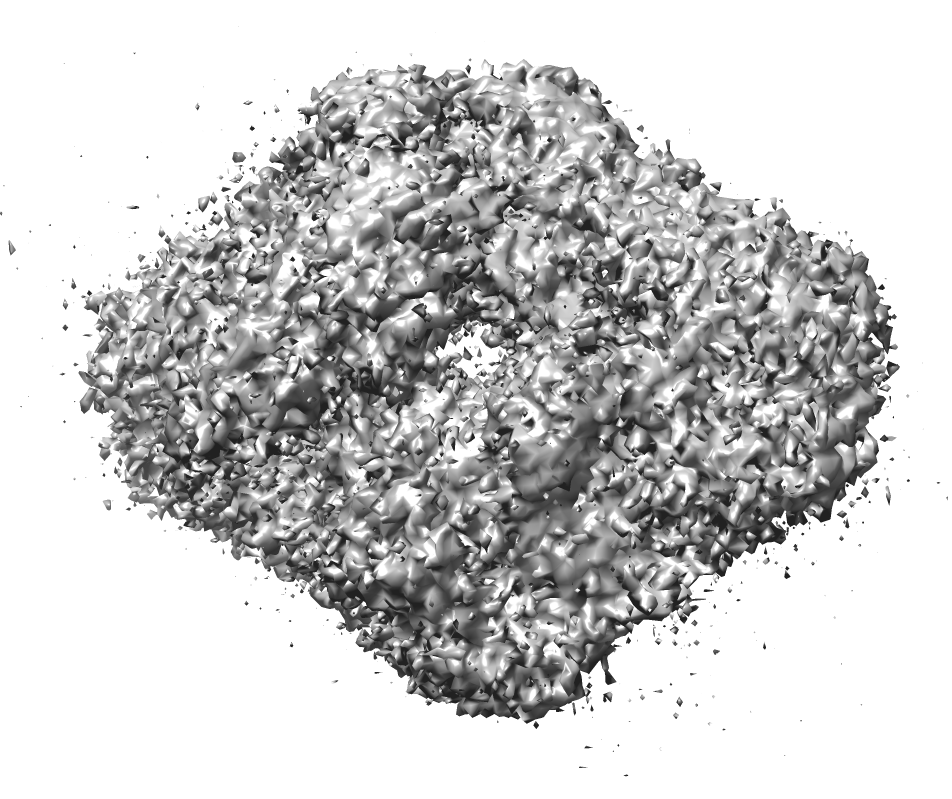
\includegraphics[height=2.5cm]{figures/5a1a_quartercov_uniformS2_noise0_apr_.png}
        \caption{}\label{fig:5a1a-noise0-reconstruction-recovered}
    \end{subfigure}
    \hfill
    \begin{subfigure}[b]{0.15\linewidth}
        \centering
        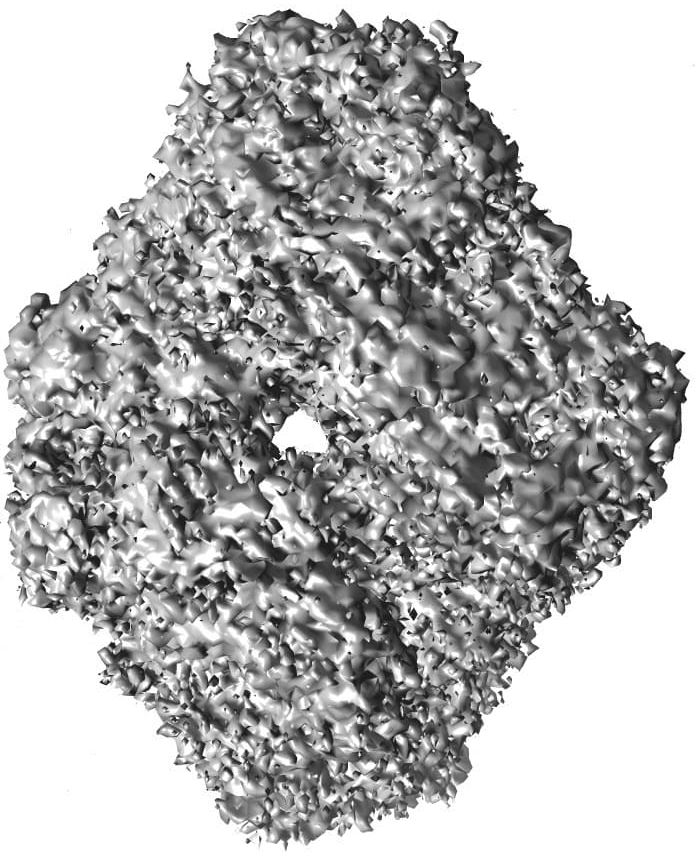
\includegraphics[height=2.5cm]{figures/5a1a_quartercov_uniformS2_noise16_apr_.png}
        \caption{}\label{fig:5a1a-noise16-reconstruction-recovered}
    \end{subfigure}
    \hfill
    \begin{subfigure}[b]{0.30\linewidth}
        \centering
        %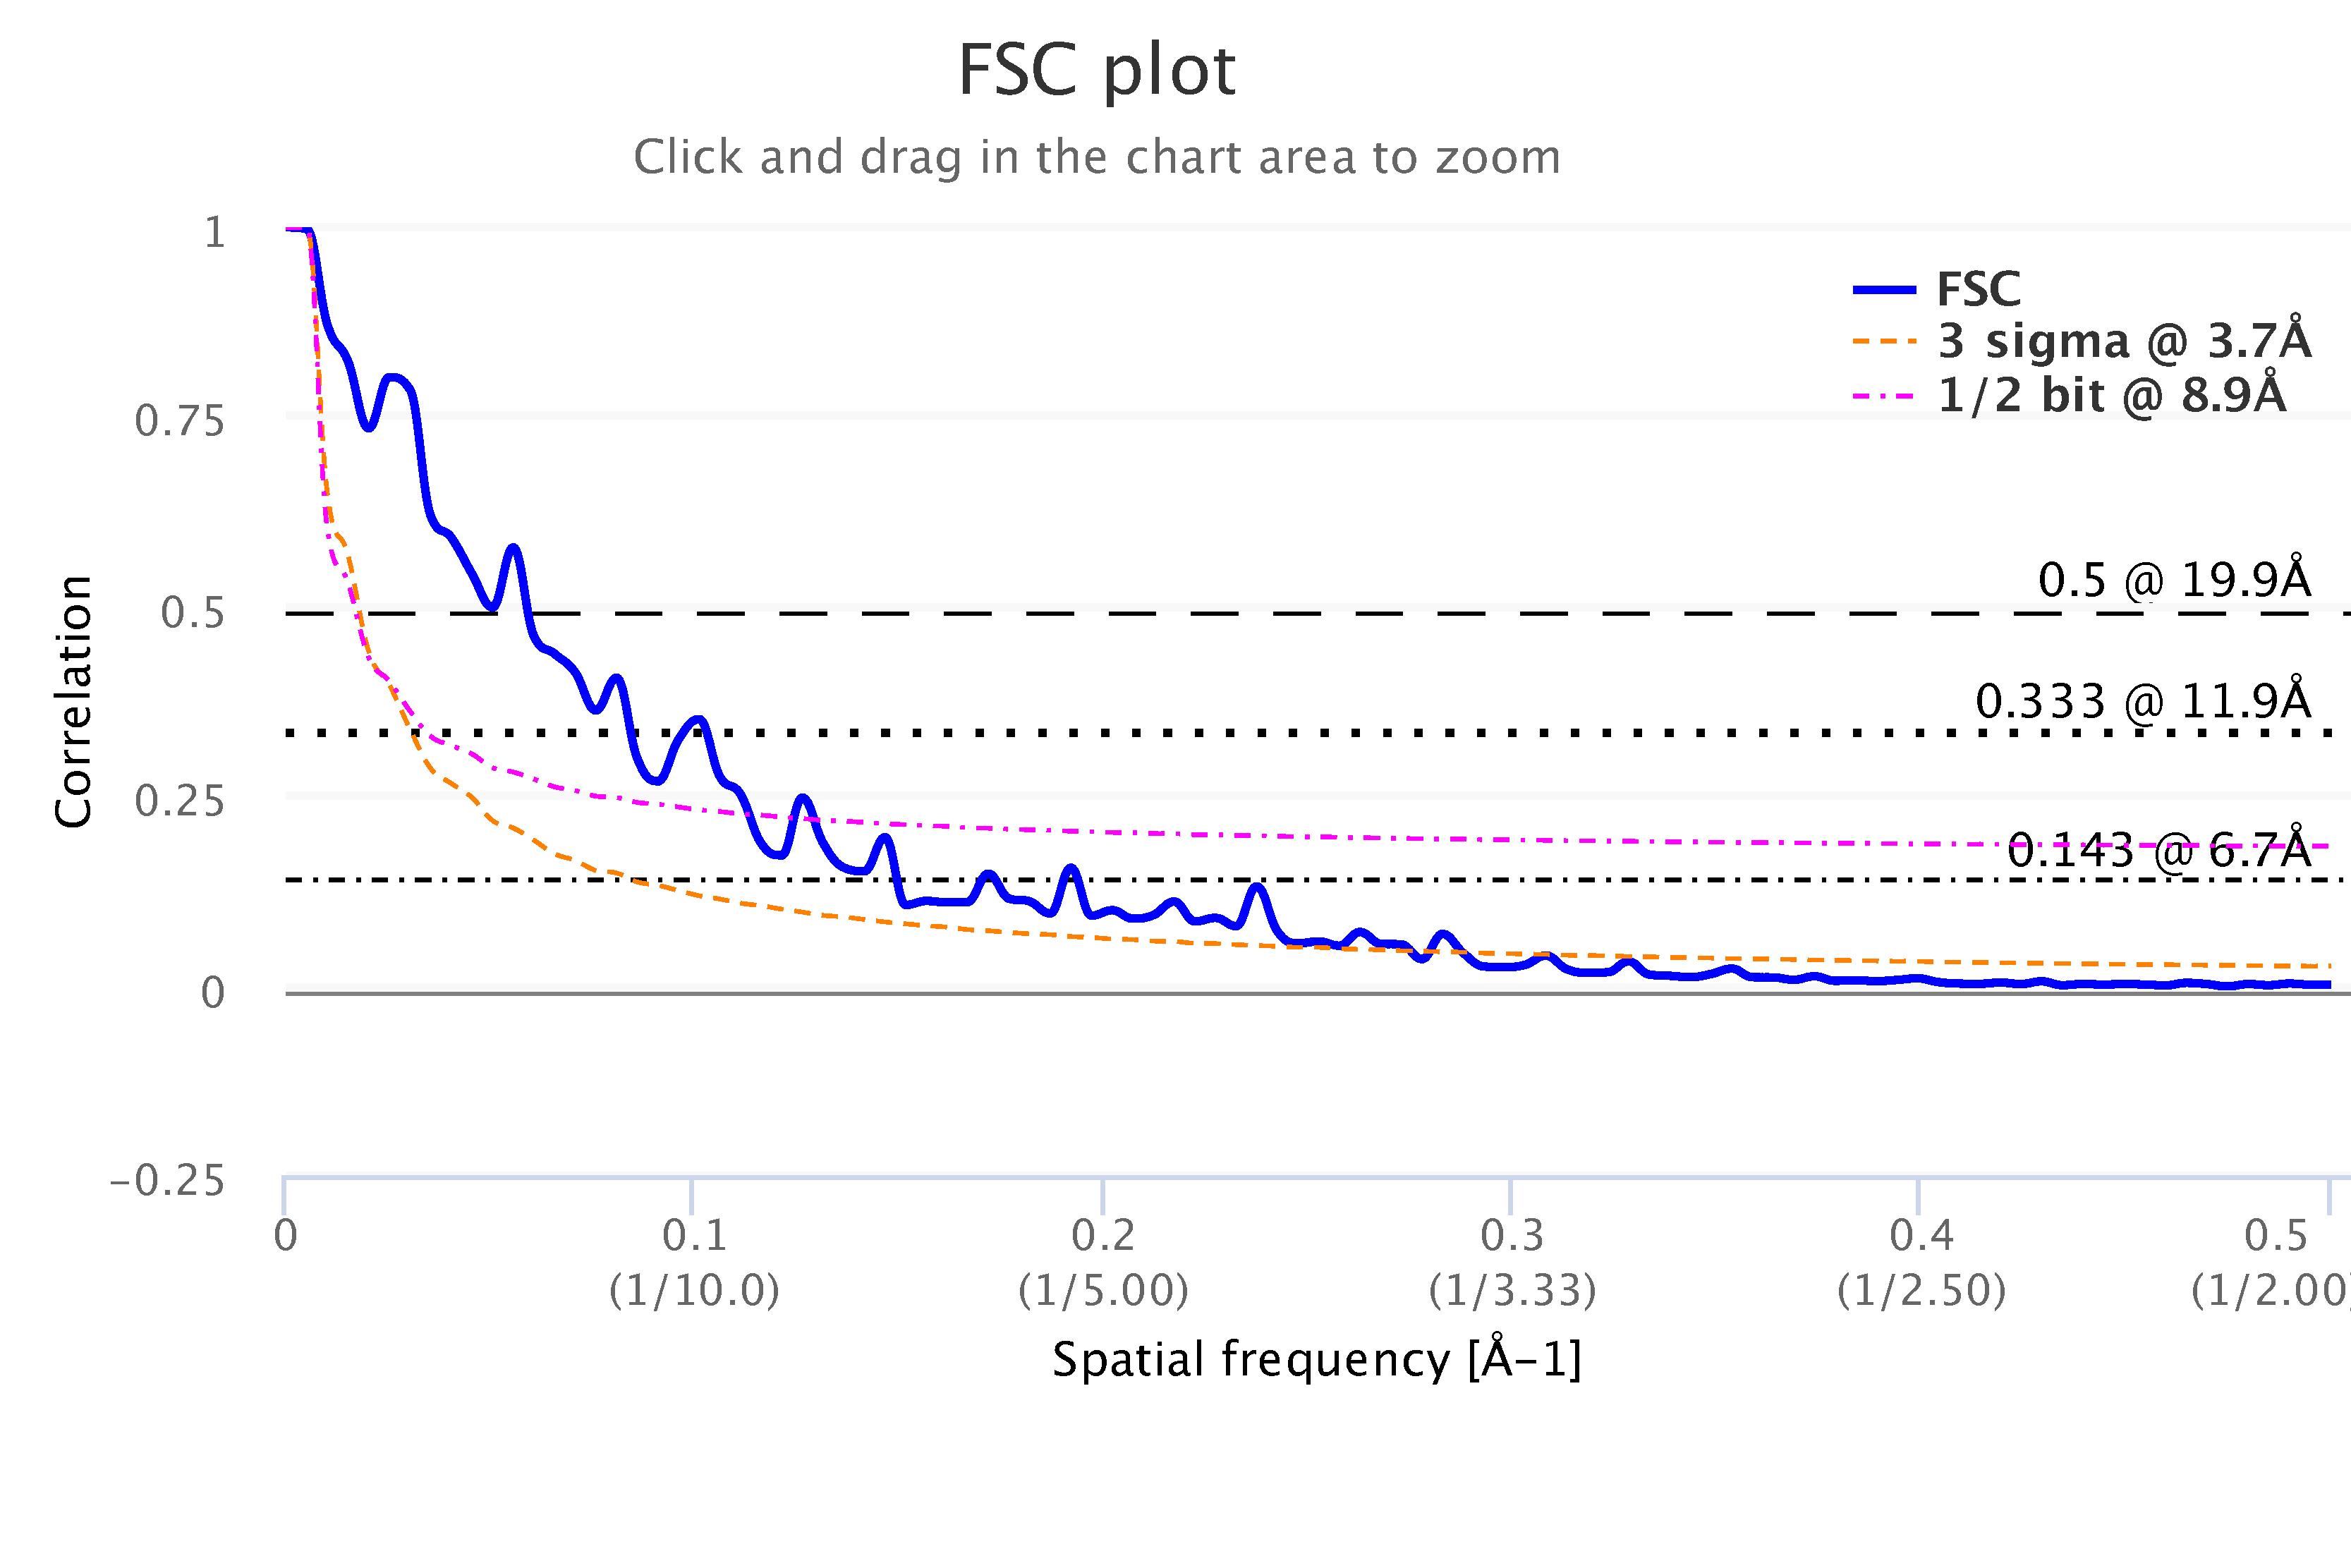
\includegraphics[height=3cm]{figures/FSC_5a1a_fin_vs_init.pdf}
        %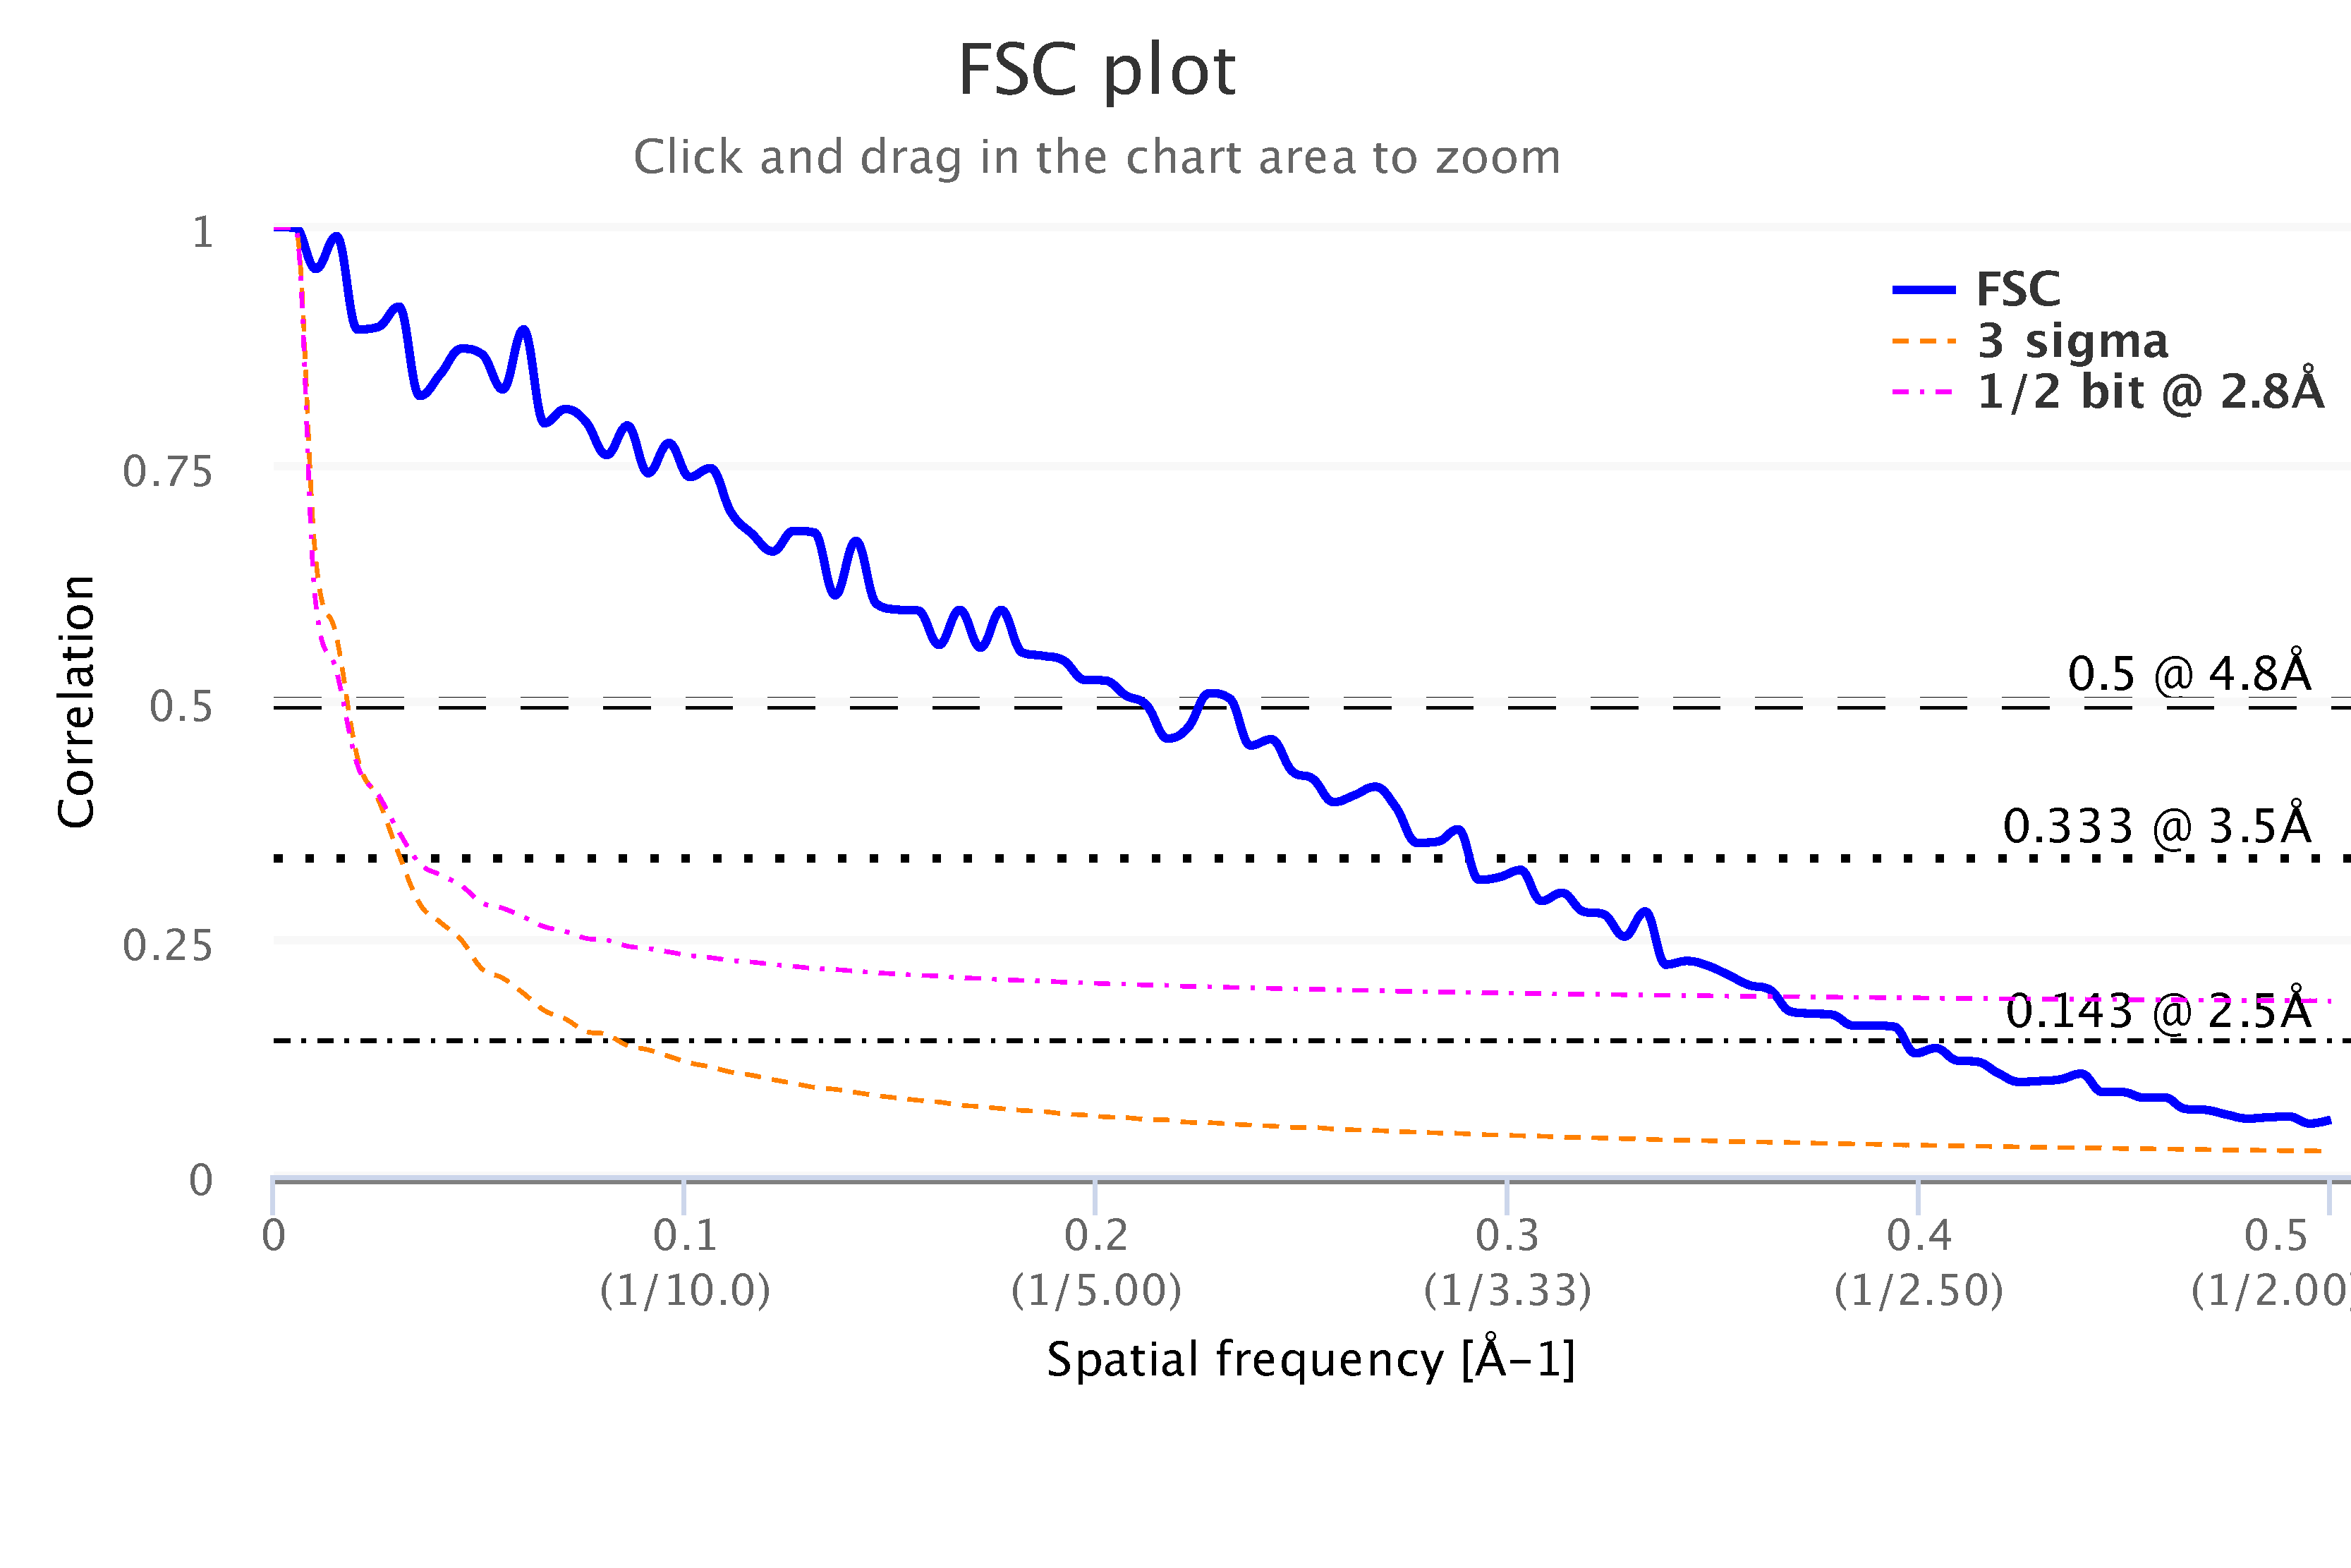
\includegraphics[height=3cm]{figures/r5a1a_quartercov_uniformS2_noise0_halfInplane_FSC_apr_init.pdf}
        % \includegraphics[height=2cm]{figures/5a1a_quartercvg_uniformS2_noise0_FSC_apr_init_customFSC.pdf}
        \includegraphics[height=2.5cm]{figures/5a1a_quartercvg_uniformS2_noise0_FSC_apr_init_customFSC2.pdf}
        \caption{}
    \end{subfigure}
    \caption{%
        Density maps $\widehat{\x}$ reconstructed from ground-truth (a,f), random (b,g), and recovered (c,d,h,i) orientations.
        Orientations were recovered from noiseless (c,h) or noisy projections (d,i).
        %While orientations were recovered from noisy projections, (e) was reconstructed from noiseless projections.
        The Fourier shell correlations (e,j) show the resolutions of the densities reconstructed from recovered orientations (w.r.t.\ ground-truth densities, shown in \figref{density-map:5j0n:ground-truth},d).
        % \lau{Suggestions: 3. filter volumes at the resolution indicated by the FSC at 0.5 (commonly done in the field),}
        \lau{4. add short captions.}
    }\label{fig:reconstructions}
\end{figure}

%\todo{HERE AND NOT IN THE DISCUSSION. More details. What happened otherwise? We want to say it's an ASTRA issue not something with our method.}\banjac{I think ASTRA tools for reconstruction have one coordinate system and our protein is reconstructed in another. The alignment that we do as a last step of the pipeline is actually the alignment to ASTRA coordinate system. I am not sure if modifying}\lau{Yeah but I wouldn't blame ASTRA at all, it's dangerous territory. There is just an engineering problem we haven't been able to solve, let's not blame well-know, widely-used existing packages out there if possible.}\mdeff{Put it as you think is best. ;)}\banjac{I will take one more look at it.}\mdeff{Great! Thanks for the investigation. Even if you can't exactly confirm, it's a good hypothesis. Leaving it at ``unknown reason'' is suspicious from a reader's POV.}


%we  were used for reconstruction. just direct hence less robust. I think it's a good idea to write this, \ie that the quality of reconstruction is likely to improve with a more robust algorithm,A state-of-the-art attempt would do it with more than $10^5$ projections and a more robust iterative reconstruction algorithm, such as those discussed in \secref{introduction}. \todo{But it's ok to compare reconstructions from true and recovered orientations.}\mdeff{Laurène, could you write something about how ASTRA is a naive reconstruction method (compared to the SOTA discussed in the intro), and that we did it only to get a crude idea? Or something along those lines. ;)}\lau{Not naïve actually,  but I'm wondering if we should not put that in the discussion/conclusion.}\mdeff{I think it's important here for people to interpret those reconstructions. They are are just here to evaluate how good orientation recovery is. And will we even discuss reconstruction in the discussion/conclusion?}
%For an unknown reason, we had to align the recovered orientations with \eqnref{orientation-recovery-error} before feeding them to ASTRA.


%\banjac{Using the ASTRA toolbox, we first create a 3D parallel beam geometry specified by 3D vectors.
%These 3D vectors are our aligned recovered orientations that are converted to a 12-dimensional vector which consists of triplets describing ray direction, the center of detector, the vector from detector pixel (0,0) to (0,1), and the vector from detector pixel (0,0) to (1,0)\footnote{https://www.astra-toolbox.com/docs/geom3d.html}.
%The center of detector was assumed to be at (0,0) and the rest of 9 values are received from converting Euler angles to a rotation matrix.
%This projection geometry is called \texttt{parallel3d} and is used to create projection geometry.
%The volume geometry is created using the 3D GPU algorithm called \texttt{BP3D\_CUDA} and the projection geometry we previously built.}

%Reconstruction is most affected by the presence of noise, due to the degraded estimation of distances.

%\mdeff{Story: pipeline works but better distance estimation is needed for SOTA reconstruction.
%Method is however promising because learned distance is robust to perturbations and recovery works if distance works.}


%Note that $L_\text{OR} \approx 0.03$ is higher than the $L_\text{OR} \approx 0.01$ in \figref{results:distance-estimation:shift} due to re-running the pipeline from scratch which includes different dataset splitting into training, validation and test sets which causes these losses to have different values.
%\mdeff{Why is $L_\text{OR} = 0.05$ while it is $0.01$ in \figref{results:distance-estimation:noise}?
%\banjac{Thanks for notice! I didn't see that. I am rerunning this pipeline for this plot. Update: I reran the 5j0n pipeline with 0 and 16 noise variance and both are shifted by ~0.25 from the results we have in the noise tests... I am not sure why, however, my thinking is that it might be due to working with a different set of generated projections from the same protein (different train-val-test split). What do you think I should do? Should I write about it or rerun the noisy experiments }


% \begin{figure}[ht!]
%     \centering
%     \begin{subfigure}[t]{0.3\linewidth}
%         \includegraphics[width=\linewidth]{figures/FSC_5j0n_gt_5j0n_apr.pdf}
%         \caption{%
%             \texttt{5j0n} with noiseless projections.
%     }\label{fig:results:fsc-5j0n-noise0}
%     \end{subfigure}
%     \hfill
%     \begin{subfigure}[t]{0.3\linewidth}
%         \includegraphics[width=\linewidth]{figures/FSC_5j0n_gt_5j0n_noisy_apr}
%         \caption{%
%         \texttt{5j0n} with noisy projections.\todo{Run the pipeline, now I miss noisy projections}
%         }\label{fig:results:fsc-5j0n-noise16}
%     \end{subfigure}
%     \hfill
%     \begin{subfigure}[t]{0.3\linewidth}
%         \includegraphics[width=\linewidth]{figures/FSC_5a1a_gt_5a1a_apr.pdf}
%         \caption{%
%         \texttt{5a1a} with noiseless projections.
%         }\label{fig:results:fsc-5a1a-noise0}
%     \end{subfigure}
%     \caption{%
%      Fourier Shell Correlation (FSC) for every reconstruction.\footnote{FSC validation server: https://www.ebi.ac.uk/pdbe/emdb/validation/fsc/}
%     }
% \end{figure}

% We observe that while distance estimation was $~25\%$ more difficult for this protein (\secref{results:distance-estimation:learned}), orientation recovery is only $~15\%$ worse; attesting to the robustness of our method.
% L_DE: 0.21/0.17=1.235
% E_OR: 0.187/0.163=1.147
% L_OR: 0.0381/0.0332=1.147

%We observe that the recovery of more accurate orientations lead to the reconstruction of more accurate density maps.
%Hence, the estimation of more accurate distances lead to more accurate reconstructions.




% \begin{figure}[ht!]
%     \centering
%     \begin{subfigure}[t]{0.3\linewidth}
%         \includegraphics[width=\linewidth]{figures/FSC_5j0n_gt_5j0n_apr.pdf}
%         \caption{%
%             \texttt{5j0n} with noiseless projections.
%     }\label{fig:results:fsc-5j0n-noise0}
%     \end{subfigure}
%     \hfill
%     \begin{subfigure}[t]{0.3\linewidth}
%         \includegraphics[width=\linewidth]{figures/FSC_5j0n_gt_5j0n_noisy_apr}
%         \caption{%
%         \texttt{5j0n} with noisy projections.\todo{Run the pipeline, now I miss noisy projections}
%         }\label{fig:results:fsc-5j0n-noise16}
%     \end{subfigure}
%     \hfill
%     \begin{subfigure}[t]{0.3\linewidth}
%         \includegraphics[width=\linewidth]{figures/FSC_5a1a_gt_5a1a_apr.pdf}
%         \caption{%
%         \texttt{5a1a} with noiseless projections.
%         }\label{fig:results:fsc-5a1a-noise0}
%     \end{subfigure}
%     \caption{%
%      Fourier Shell Correlation (FSC) for every reconstruction.\footnote{FSC validation server: https://www.ebi.ac.uk/pdbe/emdb/validation/fsc/}
%     }
% \end{figure}

% We observe that while distance estimation was $~25\%$ more difficult for this protein (\secref{results:distance-estimation:learned}), orientation recovery is only $~15\%$ worse; attesting to the robustness of our method.
% L_DE: 0.21/0.17=1.235
% E_OR: 0.187/0.163=1.147
% L_OR: 0.0381/0.0332=1.147

%We observe that the recovery of more accurate orientations lead to the reconstruction of more accurate density maps.
%Hence, the estimation of more accurate distances lead to more accurate reconstructions.
